\documentclass[11pt]{article}
\usepackage[utf8]{inputenc}
\usepackage[portuguese, russian, english]{babel}
\usepackage[T1]{fontenc}
\usepackage{subfigure} 
\usepackage{lmodern}
\usepackage{geometry}
\usepackage{authblk}
\usepackage{graphicx}
\usepackage{multicol}
\usepackage{multirow}
\usepackage{float} 
\usepackage{amsmath}

\newcommand\scalemath[2]{\scalebox{#1}{\mbox{\ensuremath{\displaystyle #2}}}}

\geometry{legalpaper, margin=1in}
\renewcommand{\arraystretch}{1.15}

\begin{document}


%%%%%%%%%%%%%%%%%%%%%%%%%%%%%%%%%%%%%%%%%%%%%%%%%%%%%%%%%%%%%%%%%%%%%%%%
%                                                                      %
%     File: Thesis_FrontCover.tex                                      %
%     Tex Master: Thesis.tex                                           %
%                                                                      %
%     Author: Andre C. Marta                                           %
%     Last modified :  2 Jul 2015                                      %
%                                                                      %
%%%%%%%%%%%%%%%%%%%%%%%%%%%%%%%%%%%%%%%%%%%%%%%%%%%%%%%%%%%%%%%%%%%%%%%%

\thispagestyle {empty}

% IST Logo - Signature A
% parameters: bb=llx lly urx ury (bounding box), width=h_length, height=v_length, angle=angle, scale=factor, clip=true/false, draft=true/false. 

\includegraphics[bb=9.5cm 11cm 0cm 0cm,scale=0.29]{IST_A_CMYK_POS}

\begin{center}
%
% Figure (Image or plot)
\vspace{1.0cm}
% height = 50 mm
%\includegraphics[height=50mm]{Figures/Airbus_A350.jpg}

% Title, author and degree
\vspace{1cm}
{\FontLb Circuit Theory and Electronics Fundamentals} \\ % <<<<< EDIT TITLE
\vspace{1cm}
{\FontSn Department of Electrical and Computer Engineering, Técnico, University of Lisbon} \\ % <<<<< EDIT COURSE
\vspace{1cm}
{\FontSn Example Laboratory Report} \\
\vspace{1cm}
{\FontSn February 27, 2021} \\ % <<<<< EDIT DATE (corresponds to date of oral examination)
%
\end{center}


\maketitle

\renewenvironment{abstract}[1]
  {\bigskip\selectlanguage{#1}%
   \begin{center}\bfseries\abstractname\end{center}}
  {\par\bigskip}

\begin{abstract}{english}
    In this report, we show a concise analysis of a 4 single mesh circuit through mesh and nodal analysis. Hitherto Ngspice has been considered a good circuit analyser and thus chosen it was to run the same circuit for comparison with the aforementioned theoretical analysis.
\end{abstract}

{
\begin{flushright}
\begin{otherlanguage*}{russian}
\itshape
"Уж небо осенью дышало,\\
Уж реже солнышко блистало,\\
Короче становился день,\\
Лесов таинственная сень\\
С печальным шумом обнажалась,\\
Ложился на поля туман,\\
Гусей крикливых караван\\
Тянулся к югу: приближалась\\
Довольно скучная пора;\\
Стоял ноябрь уж у двора."\\
\textit{Пушкин А.С.}
\end{otherlanguage*}
\end{flushright}

}
\cleardoublepage
\tableofcontents
\addcontentsline{toc}{section}{\listtablename}
\listoftables
\addcontentsline{toc}{section}{\listfigurename}
\listoffigures
\cleardoublepage

\section{Introduction}
The main goal of this laboratory assignment is to design, implement and analyse a band-pass filter (BPF) using an OP-AMP (operational amplifier) having in mind that it should have a good relation efficiency-price. The final objective was to get a central frequency of $1kHz$ for the output signal and a voltage gain of $40dB$ and the circuit's efficiency will be measured considering these objectives that were set. \\

So, in order to evaluate the relation efficiency-price of the built circuit, we will use a merit figure that considers the total cost of the circuit and the deviation to the desired gain and central frequency, defined as:

\begin{equation}
    M = \frac{1}{cost \cdot |40 - gain| \cdot |1000 - central freq.|}
    \label{merit}
\end{equation}

To calculate the total cost associated to this circuit, one considered that it equals the sum of the cost of the resistors, capacitors and transistors which is given by:

\begin{table}[H]
    \centering
    \begin{tabular}{|c|c|}
        \hline
        \textbf{Component} &  \textbf{Price}\\
        \hline
        Resistors & 1 MU $k\Omega^{-1}$ \\ \hline
        Capacitors & 1 MU $\mu F^{-1}$ \\ \hline
        Transistors & 0.1 MU transistor$^{-1}$\\
        \hline
    \end{tabular}
    \caption{Price table for the components used}
    \label{tab:price}
\end{table}

The central frequency represented on eq. \eqref{merit} can be directly calculated from the definition of transfer function for this system and it is given by the geometric mean of the lower and higher cutoff frequencies:

\begin{equation}
    central freq. = \sqrt{f_H f_L}
\end{equation}

in which $f_H$ corresponds to the higher cutoff frequency and $f_L$ to the lower cutoff frequency. Finally, the value for the voltage gain used on eq. \eqref{merit} is easily obtained as the correspondent voltage value for the central frequency obtained. \\

The circuit used to implement this band-pass filter using an OP-AMP can be divided in 3 main regions as it can be seen on Fig. \ref{initialscheme}

\begin{figure}[H]
    \centering
    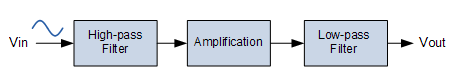
\includegraphics{esquemabunituh.PNG}
    \caption{Simplified scheme to present the 3 regions in which the circuit used can be divided}
    \label{initialscheme}
\end{figure}

The first part, a high-pass filter stage, will essentially have a resistor and a capacitor (i.e. will only pass signals with a frequency higher than a certain cutoff frequency, $f_L$). This part is followed by an amplification unit which will have the main objective of increasing the output voltage gain and which counts with an OP-AMP and two resistors. Finally, one implemented a low-pass filter stage on the circuit which operates on the opposite way of the high-pass filter, i.e. blocks all the signals with a frequency higher than a certain cutoff frequency, $f_H$). \\

As it is trivial, the high-pass filter and the low-pass filter blocking simultaneously frequencies lower than $f_L$ and higher that $f_H$ will act as a band-pass filter as desired. \\

Furthermore, and considering all the points mentioned before, the circuit used for this purpose was the following:


The results were obtained through a theoretical analysis, in which one predicted the output by using a theoretical method that suited the real circuit and through a simulation that was made using \textit{Ngspice}. The results obtained through both methods will be analysed throughout the report. However, because the models used in \textit{Ngspice} are more correct than the ones used on the theoretical analysis, any type of optimization was done almost exclusively in the simulation analysis.\\
\section{Theoretical Analysis}
\label{sec:theo}
\subsection{Nodal Analysis at $t<0$}
\label{sec:1st}
First of all, one can start by applying the nodal analysis method at $t<0$ to find the voltages of all nodes and, afterwards, using Ohm's law, the currents that flow through each branch of the circuit. Note that the labels used to refer to each node and branch are exactly the same as presented in Fig. \ref{fig:bigscheme}.

So, the next step is to write linearly indepedent equations that will allow us to get the voltages at each node. Note that for $t<0$, we will have $u(t) = 0 \Longrightarrow I_c = 0$ and so, by applying the condition associated with the independent voltage source, one will have a constant value for $v_s(t)$, such that $v_s (t) = V_s$ for $t<0$ (as it can be seen in the expression for the independent voltage source in Fig. \ref{fig:bigscheme}.

\begin{equation}
    \begin{cases}
        V_1 - V_4 = V_s \hspace{15px} \text{(independent voltage source)}\\
        (V_2-V_1)G_1 + (V_2-V_3)G_2 + (V_2-V_5)G_3 = 0 \hspace{15px}\text{(node 2)}\\
        (V_3 - V_2)G_2 + (V_5 - V_2)K_b = 0 \hspace{15px}\text{(node 3)}\\ 
        V_4 = 0 \hspace{15px}\text{(node 4 assigned to GND)}\\
        (V_5-V_2)G_3 + (V_5-V_4)G_4 + (V_5-V_6)G_5 + (V_8-V_7)G_7 = 0 \hspace{15px}\text{(supernodal equation)}\\
        (V_6-V_5)G_5 + (V_2-V_5)K_b = 0 \hspace{15px}\text{(node 6)}\\
        (V_7-V_4)G_6 + (V_7-V_8)G_7 = 0 \hspace{15px}\text{(node 7)}\\
        V_5 - V_8 = (V_7-V_4)K_dG_6 \hspace{15px}\text{(restriction equation involving dependent voltage source)}
    \end{cases}
\end{equation}

Note that the last equation of this system, the restriction equation involving the current-controlled voltage source, urges as the result of the combination of two equations. As shown in Fig. \ref{fig:bigscheme}, one can write $V_d$ as:

\begin{equation}
    V_d = K_d I_d
\end{equation}

and also:

\begin{equation}
    V_d = V_5 - V_8
\end{equation}

Because $I_d$ is the current which flows through the resistor $R_6$ (one could write an equivalent equation by using the resistor $R_7$, as the current flowing through it is exactly the same), one can easily write, using Ohm's Law:

\begin{equation}
    I_d = (V_7 - V_4)G_6
\end{equation}

Combining these 3 equations, one can obtain the restriction equation used in the previous system:

\begin{equation}
    V_d = V_5 - V_8 = (V_7 - V_4)G_6 K_d
\end{equation}

Converting this system of equations to its matricial form, one can obtain:

\begin{equation}
    \begin{bmatrix}
     1 &  0      &  0 &    -1  &     0      &  0  &  0    &  0\\
     -G_1 & G_1+G_2+G_3 & -G_2  & 0   &  -G_3       &  0  &  0    &  0\\
     0   & -G_2-K_b    & G_2  & 0   &   K_b       &  0  &  0    &  0\\
     0   & 0        & 0   & 1 & 0       &  0  & 0   & 0\\
     0   & -G_3      &  0 &  -G_4  &   G_3+G_4+G_5 & -G_5 &  -G_7    & G_7\\
     0   & K_b       & 0  &  0    & -G_5-K_b     & G_5  & 0     & 0\\
     0   & 0        & 0  & -G_6   &  0         & 0   & G_6+G_7 & -G_7\\
     0   & 0        & 0  &  -K_dG_6    &  1         & 0   & K_dG_6     & -1
    \end{bmatrix} 
    \begin{bmatrix}
        V_1\\
        V_2\\
        V_3\\
        V_4\\
        V_5\\
        V_6\\
        V_7\\
        V_8
    \end{bmatrix}
    = 
    \begin{bmatrix}
        V_s\\
        0\\
        0\\
        0\\
        0\\
        0\\
        0\\
        0
    \end{bmatrix}
\label{eqnodos2}
\end{equation}

The matrix system \ref{eqnodos2} is composed of a very sparse matrix, thus we also advise for using correspondingly adapted sparse matrix solvers if possible, but this is already out of the scope of this discipline and laboratory. Getting back to the point, the solution to the matrix system is,

%V1 & 5.038475019720000E+00  \\ \hline
V2 & 4.758223649291032E+00 \\ \hline
V3 & 4.170534768621250E+00 \\ \hline
V5 & 4.798515115188197E+00 \\ \hline
V6 & 5.646841168887640E+00  \\ \hline
V7 & -1.834523049106916E+00 \\ \hline
V8 & -2.756787388808905E+00 \\ \hline


Finally, to find the currents in the circuit, one can apply Ohm's law as one knows all the resistor values and the voltages in all of the circuit's nodes (presented in \eqref{eqsol}. \\

Labeling the positive and negative terminals of each component as inserted in \textit{Ngspice}, and as it can be seen in Fig. something, one can obtain

\begin{table}[H]
    \begin{minipage}{.5\textwidth}
      \begin{equation} \Vec{b} = \begin{bmatrix}  5.0385\\  4.7582\\  4.1705\\      -0\\  4.7985\\  5.6468\\ -1.8345\\ -2.7568 \end{bmatrix} \label{eqsol} \end{equation}
    \end{minipage}
    \begin{minipage}{.5\textwidth}
      \centering
      \begin{tabular}{c|c}
        \hline
          Branch &  Current (A) \\
          \hline
          I(R1) & -0.000269\\
I(R2) & 0.000283\\
I(R3) & -0.000013\\
I(R4) & -0.001172\\
I(R5) & -0.000283\\
I(R6) & 0.000902\\
I(R7) & 0.000902\\
I(Vs) & -0.000269\\
I(Vd) & -0.000902\\
Id  & 0.000902\\
Ib & -0.000283\\
Ic & 0.000000\\

          \hline
      \end{tabular}
    \end{minipage}
    \caption{Theoretical solution for voltages for all nodes and current for all branches for $t<0$.}
    \label{tab:current}
\end{table}


\subsection{$R_{eq}$ and time constant $\tau$}
Next up, we need to determine the equivalent resistance, $R_eq$, as seen from the capacitor terminals to find the time constant associated with this circuit, $\tau = R_{eq}C$, so that one can analyse, afterwards, the natural and the forced solution of the circuit. \\

To do that, one can start by "shutting down" the independent voltage source of the circuit, $V_s$, by making it $V_s = 0$, i.e., replacing it by a short circuit. Afterward, as we want to calculate $R_{eq}$ as seen by the terminals of the capacitor, one should now substitute the capacitor by a voltage source with value $V_x = V_6 - V_8$, where one can use the values obtained in section \ref{sec:1st} for $V_6$ and $V_8$. This whole process is adopted because the value $R_{eq}$ which we are seeking is nothing more than the Thévenin Resistance, $R_{th}$, of the circuit as seen by the terminals of the capacitor. \\

Rewriting the system of equations with this new constraints (knowing the value for $V_x$ and imposing $V_s = 0$), one can write the system as:

\begin{equation}
    \begin{bmatrix}
     1 &  0      &  0 &    -1  &     0      &  0  &  0    &  0\\
     -G_1 & G_1+G_2+G_3 & -G_2  & 0   &  -G_3       &  0  &  0    &  0\\
     0   & -G_2-K_b    & G_2  & 0   &   K_b       &  0  &  0    &  0\\
     0   & 0        & 0   & 1 & 0       &  0  & 0   & 0\\
     0   & -G_3+K_b      &  0 &  -G_4  &   G_3+G_4-K_b & 0 &  -G_7    & G_7\\
     0   & 0       & 0  &  0    & 0     & 1  & 0     & -1\\
     0   & 0        & 0  & -G_6   &  0         & 0   & G_6+G_7 & -G_7\\
     0   & 0        & 0  &  -K_dG_6    &  1         & 0   & K_dG_6     & -1
    \end{bmatrix} 
    \begin{bmatrix}
        V_1\\
        V_2\\
        V_3\\
        V_4\\
        V_5\\
        V_6\\
        V_7\\
        V_8
    \end{bmatrix}
    = 
    \begin{bmatrix}
        0\\
        0\\
        0\\
        0\\
        0\\
        V_x\\
        0\\
        0
    \end{bmatrix}
\label{eqnodos}
\end{equation}

Which take us to this result:

\begin{equation}
    \begin{bmatrix}
        V_1\\
        V_2\\
        V_3\\
        V_4\\
        V_5\\
        V_6\\
        V_7\\
        V_8
    \end{bmatrix}
    = 
    \begin{bmatrix}
        0\\
        0\\
        0\\
        0\\
        0\\
        8.40363\\
        0\\
        0
    \end{bmatrix}V
\end{equation}

Now that one obtained the values for every node voltage, and having in mind that $I_x$ can be written as $I_x = -(I_b+I_5)$:

\begin{equation}
\begin{cases}
    I_b = K_b(V_2 - V_5) = 0mA\\
    I_5 = (V_6 - V_8)G_5 \approx -2.80 mA
\end{cases}
    \Longrightarrow I_x = -I_5 = 2.80 mA
\end{equation}

Now that one obtained the values of $V_x$ and $I_x$, one can finally obtain the value for $R_eq$, which can be written as:

\begin{equation}
    R_{eq} = \frac{V_x}{I_x} \approx 3.0014 k\Omega
\end{equation}

Finally, as for RC circuits, the time constant can be expressed as:

\begin{equation}
    \tau = R_{eq}
\end{equation}

one can obtain that for this specific circuit, $tau$ can be written as:

\begin{equation}
    \tau \approx 3.0516 ms
\end{equation}
\subsection{Node analysis for $t\geq0$ - natural solution for $v_6(t)$}
Analysing now the circuit in $t>0$ in order to determine the evolution of the voltage on node 6, $V_6$, with time, $v_6(t)$, one can start by determining its natural solution. To do that, we start by assuming the general form of this solution which can be written as:

\begin{equation}
    v_{6n}(t) = v_{6n} (t\to\infty) + (v_{6n}(t = 0) - v_{6n}(t\to\infty))e^{-\frac{t}{\tau}}
\label{generalfor}
\end{equation}

in which $\tau$ represents the time constant for this RC circuit, i.e., $\tau = R_{eq}C$, as calculated on the previous section.\\

Starting by $v_6 (t=0)$, the initial condition for the solution which we are seeking is $V_x$, the voltage obtained in the last section for the voltage source by which one replaced the capacitor. So on, using the last section results, as $V_x = V_6 - V_8$ and $V_8 = 0$, one can infer that $V_x = V_6$, and so one can conclude that $v_6(t=0) = V_x$. \\

Only $v_(t\to\infty)$ remains unknows. To find it, one can run again the nodal analysis system of equations with $V_s = 0$, as we are searching only for the natural solution by now. So, one can write the equivalent matricial equation for $t\to\infty$ as:

\begin{equation}
    \begin{bmatrix}
     1 &  0      &  0 &    -1  &     0      &  0  &  0    &  0\\
     -G_1 & G_1+G_2+G_3 & -G_2  & 0   &  -G_3       &  0  &  0    &  0\\
     0   & -G_2-K_b    & G_2  & 0   &   K_b       &  0  &  0    &  0\\
     0   & 0        & 0   & 1 & 0       &  0  & 0   & 0\\
     0   & -G_3+K_b      &  0 &  -G_4  &   G_3+G_4-K_b & 0 &  -G_7    & G_7\\
     0   & 0       & 0  &  0    & 0     & 1  & 0     & -1\\
     0   & K_b        & 0  & 0   &  -G_5-K_b         & G_5   & 0 & 0\\
     0   & 0        & 0  &  -K_dG_6    &  1         & 0   & K_dG_6     & -1
    \end{bmatrix} 
    \begin{bmatrix}
        V_1\\
        V_2\\
        V_3\\
        V_4\\
        V_5\\
        V_6\\
        V_7\\
        V_8
    \end{bmatrix}
    = 
    \begin{bmatrix}
        0\\
        0\\
        0\\
        0\\
        0\\
        0\\
        0\\
        0
    \end{bmatrix}
\label{eqnodos}
\end{equation}

which results in the following solution:

\begin{equation}
    \begin{bmatrix}
        V_1\\
        V_2\\
        V_3\\
        V_4\\
        V_5\\
        V_6\\
        V_7\\
        V_8
    \end{bmatrix}
    = 
    \begin{bmatrix}
        0\\
        0\\
        0\\
        0\\
        0\\
        0\\
        0\\
        0
    \end{bmatrix} V
\label{zeros}
\end{equation}

Knowing $v_{6n}(t = 0)$ and $v_{6n}(t\to\infty)$ one can now use equation \eqref{generalfor} to find the expression for the natural solution of the voltage on node 6:

\begin{equation}
    v_{6n}(t) \approx 8.4036e^{-\frac{t}{0.0030516}}
\end{equation}

Plotting the function obtained on the interval $t \in [0,20]ms$, one can get the graph shown in Fig. \ref{fig:natural}

\begin{figure}[H]
    \centering
    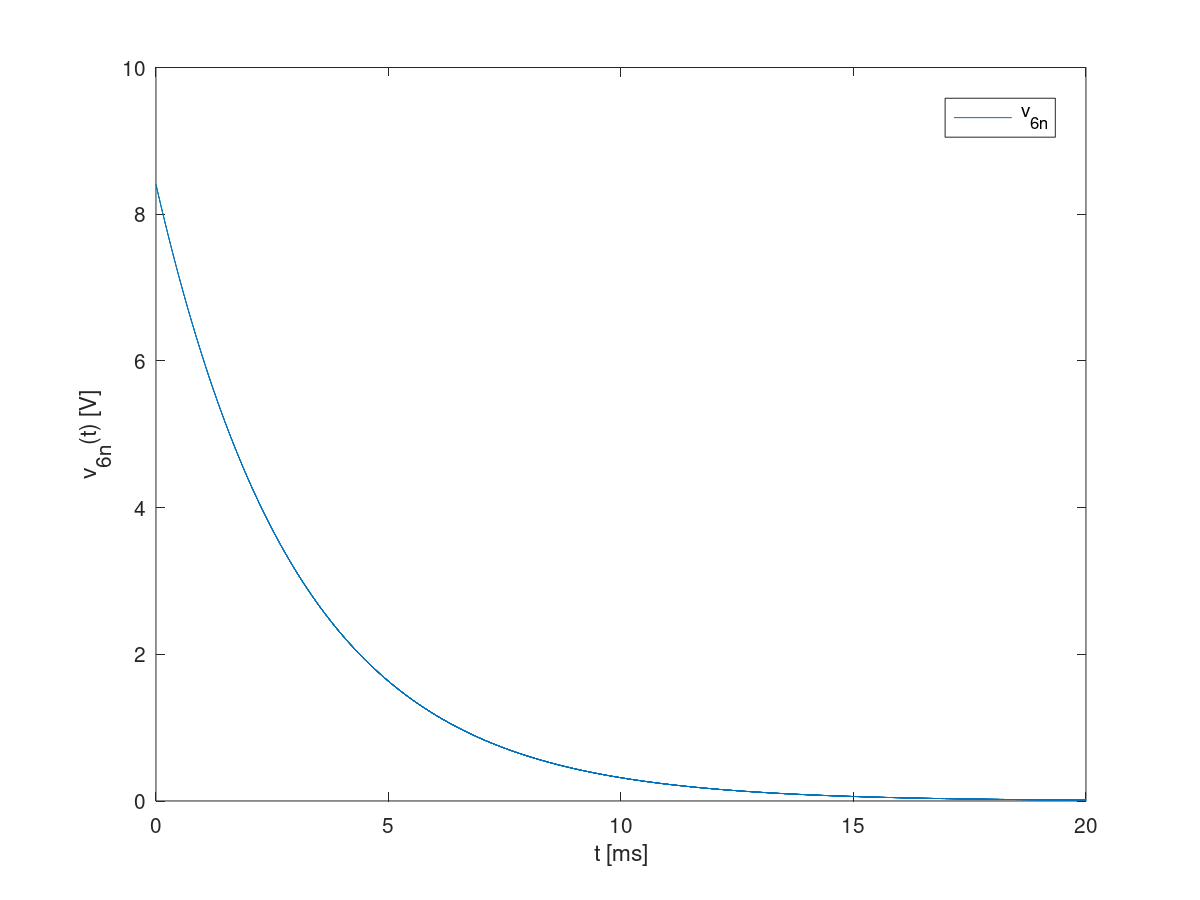
\includegraphics[width = 0.85\linewidth]{../mat/v6n.png}
        \caption{\textit{Plot of the natural solution for the voltage on node 6 in the interval $t\in[0,20]ms$ as shown on the plot}}
    \label{fig:natural}
\end{figure}
\subsection{Node analysis for $t\geq0$ - forced solution $v_6(t)$}

To complete the solution of the system, the forced solution needs to be determined. That was done using the nodal analysis method equivalent to \ref{eqnodos} but adding the current flowing thought the capacitor and changing the voltage source to it's new function ($V_s(t)=sin(2\pi f t)$ , $t\geq0$) resulting in the change of only this 3 equations.

\begin{equation}
    \begin{cases}
        V_1 - V_4 = -i e^{i 2\pi f C t} \hspace{15px} \text{(independent voltage source)}\\
        (V_5-V_2)G_3 + (V_5-V_4)G_4 + (V_5-V_6)G_5 + (V_8-V_7)G_7 + (V_8-V_6)i 2\pi f C = 0 \hspace{15px}\text{(supernodal equation)}\\
        (V_6-V_5)G_5 + (V_2-V_5)K_b + (V_6-V_8)i 2\pi f C = 0 \hspace{15px}\text{(node 6)}\\
    \end{cases}
\end{equation}

Note that the the complex phasors are being used instead of the normal sine function in order to obtain the complex amplitudes. Converting this system of equations to its matricial form, one can obtain:

\begin{equation}
\scalemath{0.8}{
    \begin{bmatrix}
     1 &  0      &  0 &    -1  &     0      &  0  &  0    &  0\\
     -G_1 & G_1+G_2+G_3 & -G_2  & 0   &  -G_3       &  0  &  0    &  0\\
     0   & -G_2-K_b    & G_2  & 0   &   K_b       &  0  &  0    &  0\\
     0   & 0        & 0   & 1 & 0       &  0  & 0   & 0\\
     0   & -G_3      &  0 &  -G_4  &   G_3+G_4+G_5 & -G_5-i 2\pi f C &  -G_7    & G_7+i 2\pi f C\\
     0   & K_b       & 0  &  0    & -G_5-K_b     & G_5+i 2\pi f C  & 0     &  -i 2\pi f C\\
     0   & 0        & 0  & -G_6   &  0         & 0   & G_6+G_7 & -G_7\\
     0   & 0        & 0  &  -K_dG_6    &  1         & 0   & K_dG_6     & -1
    \end{bmatrix} 
    \begin{bmatrix}
       V_1\\
        V_2\\
        V_3\\
        V_4\\
        V_5\\
        V_6\\
        V_7\\
        V_8
    \end{bmatrix}
    =
    \begin{bmatrix}
        -i e^{i 2\pi f C t}\\
        0\\
        0\\
        0\\
        0\\
        0\\
        0\\
        0
    \end{bmatrix}}
\label{eqnodos_forced}
\end{equation}

With the matrix defined, a program in octave was used to solve the system symbolically, to which was then substituted the frequency for $1000 Hz$ and, in order to obtain the complex amplitude, time for $0$, obtaining the values in Tab. \ref{tab:amplitude}.

The information that these complex amplitudes contain is the phase and amplitude of the oscillation, in this case forced, values that can be obtained through the complex amplitude norm and its argument, respectively, as it was done and the results are presented in Tab. \ref{tab:amplitude}.


\begin{table}[H]
    \begin{minipage}{.5\textwidth}
      \centering
      \begin{tabular}{c|c}
        \hline
     Node &  Complex Amplitude (v)\\ 
     \hline
    V(1) & -0.000000 + i(-1.000000)\\ V(2) & 0.000000 + i(-0.944378)\\ V(3) & -0.000000 + i(-0.827738)\\ V(5) & 0.000000 + i(-0.952375)\\ V(6) & -0.086752 + i(0.542623)\\ V(7) & 0.000000 + i(0.364103)\\ V(8) & 0.000000 + i(0.547147)\\ 
    \hline
      \end{tabular}
    \end{minipage}
    \begin{minipage}{.5\textwidth}
      \centering
      \begin{tabular}{c|c|c}
        \hline
          Node &  Amplitude (V) & Phase (rad)\\
          \hline
          V(1) & 1.000000 & -1.570796\\ 
V(2) & 0.944378 & -1.570796\\ 
V(3) & 0.827738 & -1.570796\\ 
V(5) & 0.952375 & -1.570796\\ 
V(6) & 0.549514 & 1.729330\\ 
V(7) & 0.364103 & 1.570796\\ 
V(8) & 0.547147 & 1.570796\\ 

          \hline
      \end{tabular}
    \end{minipage}
    \caption{Amplitudes for the forced solution osculations}
    \label{tab:amplitude}
\end{table}

With this information the forced solution can be plotted, in specific, in Fig.\ref{fig:forced}.

\begin{figure}[H]
    \centering
    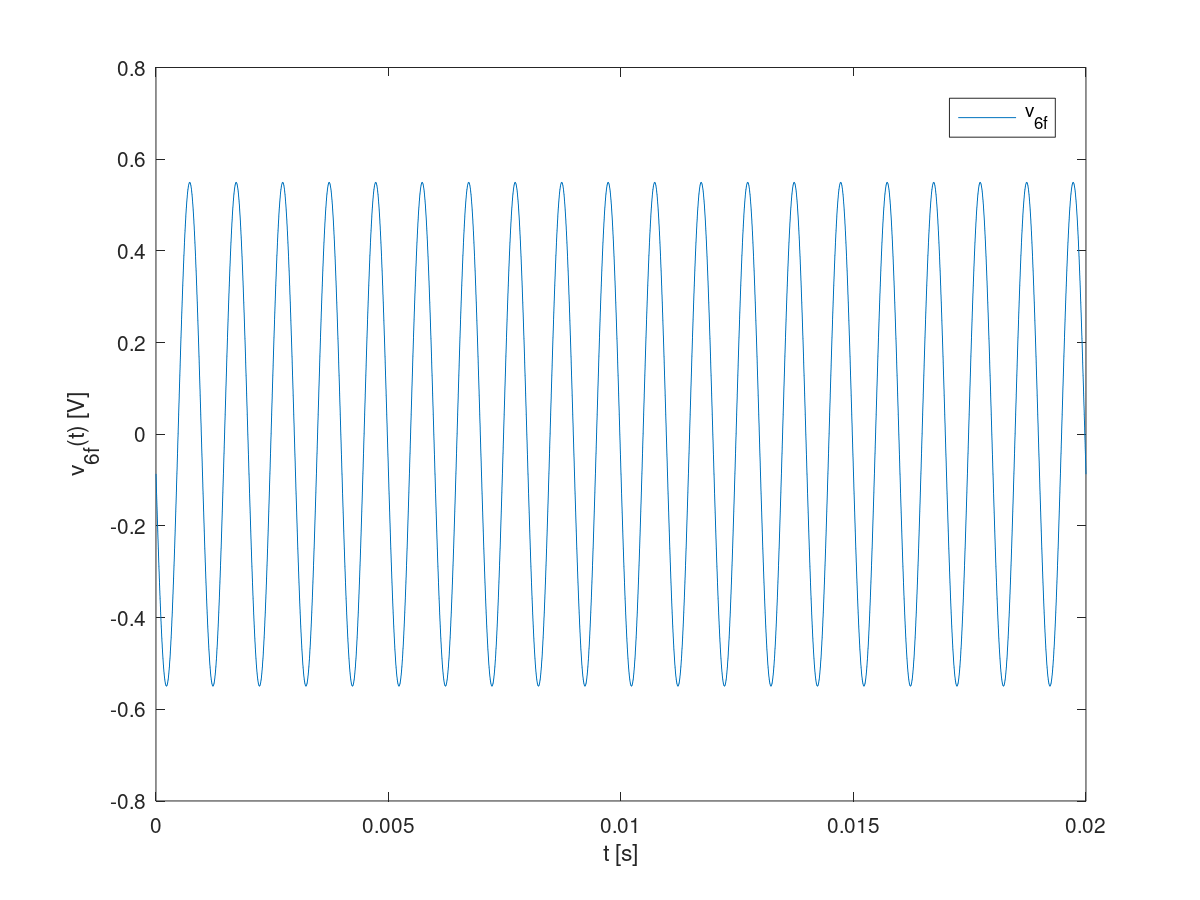
\includegraphics[width = 0.85\linewidth]{../mat/v6f.png}
        \caption{\textit{Plot of the forced solution for the voltage on node 6 in the interval $t\in[0,20]ms$ as shown on the plot}}
    \label{fig:forced}
\end{figure}

With both natural, obtained in Fig. \ref{fig:natural} and forced solutions, obtained in Fig. \ref{fig:forced} determined it's easy to add the 2 in order to obtain the complete solution, which for $V_6(t)$ is ploted in Fig. \ref{fig:complete}

\begin{figure}[H]
    \centering
    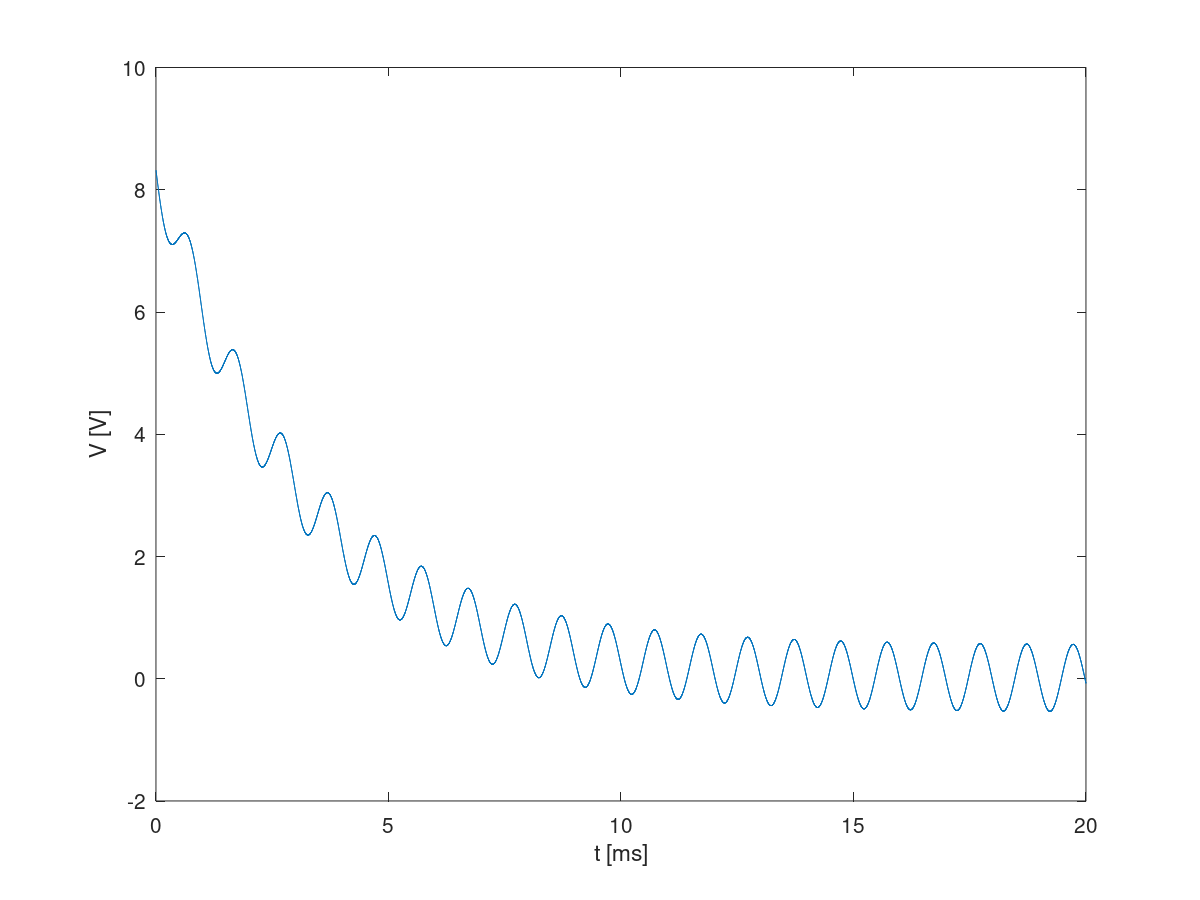
\includegraphics[width = 0.85\linewidth]{../mat/v6fn.png}
        \caption{\textit{Plot of the complete solution for the voltage on node 6 in the interval $t\in[0,20]ms$ as shown on the plot}}
    \label{fig:complete}
\end{figure}

For further understanding the behaving of the system, the voltage in node 6 and the input voltage can both be ploted for before and after $t=0$, by merging the results from the previous theoretical analysis, resulting in what is seen in Fig. \ref{fig:tudo}.

\begin{figure}[H]
    \centering
    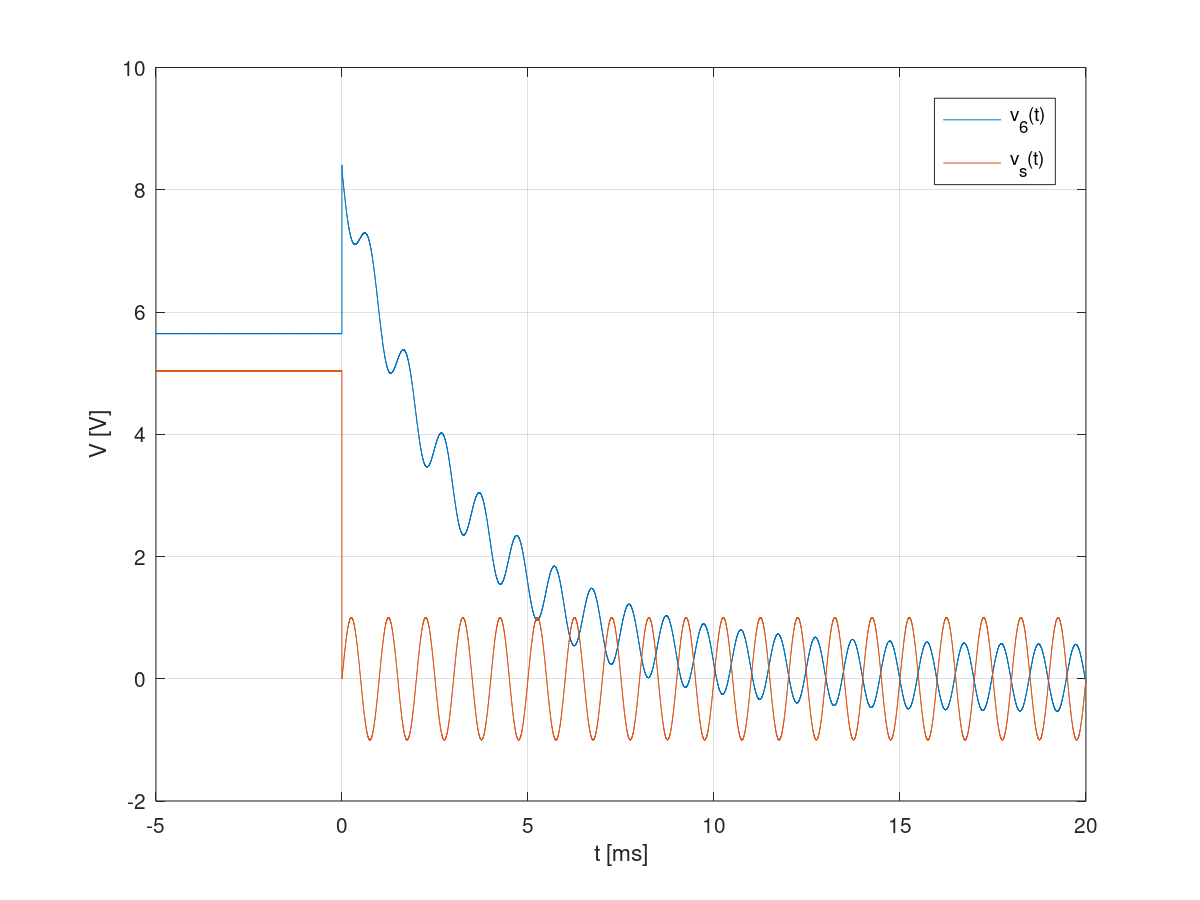
\includegraphics[width = 0.85\linewidth]{../mat/v6totsze.png}
        \caption{\textit{Plot of the complete solution for the voltage on node 6 and the input voltage  in the interval $t\in[-5,20]ms$ as shown on the plot}}
    \label{fig:tudo}
\end{figure}

As expected we can see that the discontinuity in the voltage source causes a discontinuity in the voltage in node 6, just not as intense and the system takes some time to reach the equilibrium and adapt to a behavior similar to its source. It's also notable that these 2 voltages are separated in phase by half a period.

\subsection{Magnitude and Phase as Functions of Frequency}

Once the system was solved symbolically, the complex amplitudes in function of the frequency could be obtain symbol by keeping $t=0$, and varying only the frequency, which in this case was done in the interval between $0.1$ and $10^6$ Hz. This time the goal was specifically to get the magnitude and the phase, instead of the complex amplitude, so as before were used the norm and the argument.

\begin{figure}[H]
    \centering
    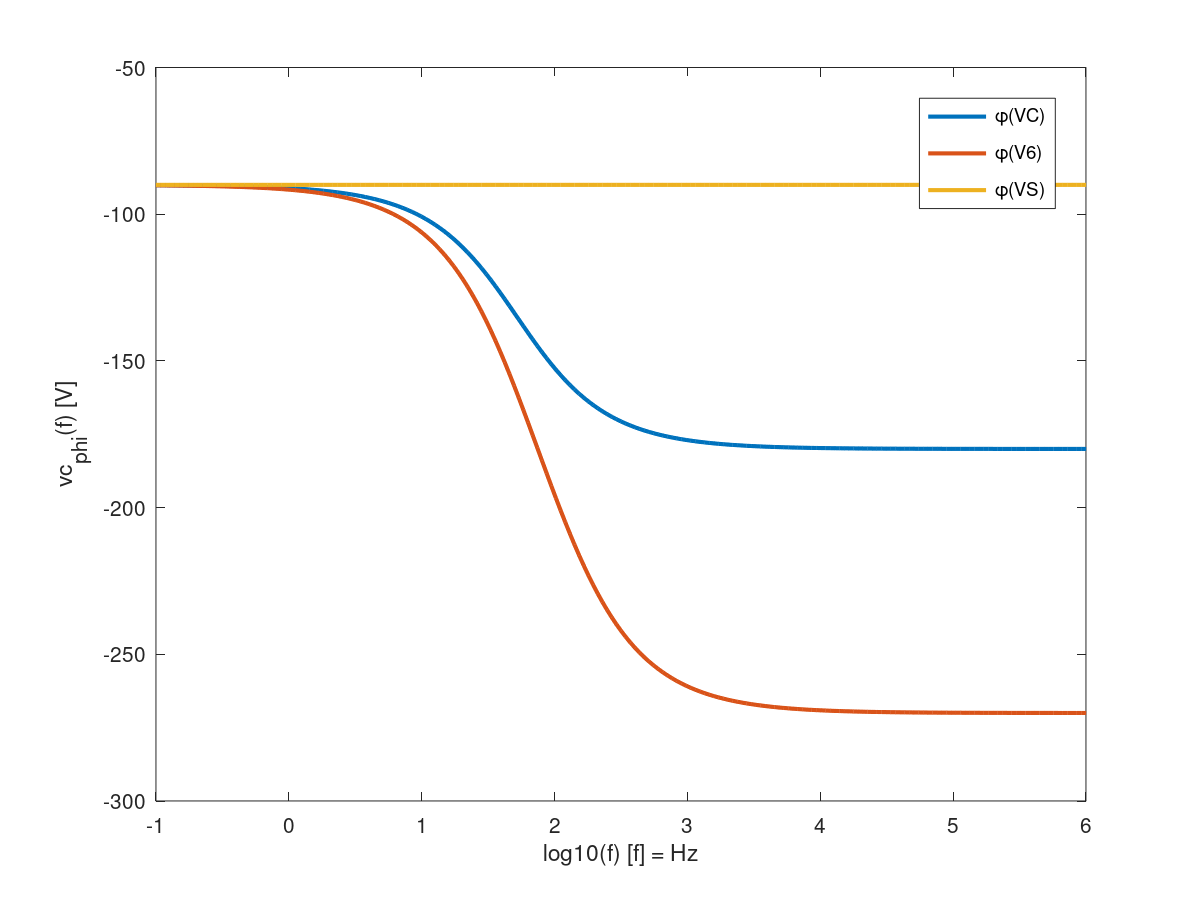
\includegraphics[width = 0.85\linewidth]{../mat/vcphi.png}
        \caption{\textit{Plot of the phase in function of the frequency. The frequency is presented in a logarithmic scale, contrary to the phase which is in linear scale in degrees.}}
    \label{fig:phase}
\end{figure}

As expected the phase for the voltage source is not dependent on the frequency, which was clear in the formula used to define it. More interestingly, the phase for both $V_c$ and $V_6$ seem to decrease around $50Hz$, stabilizing in a quarter and half a period, respectively, for higher frequencies.  


\begin{figure}[H]
    \centering
    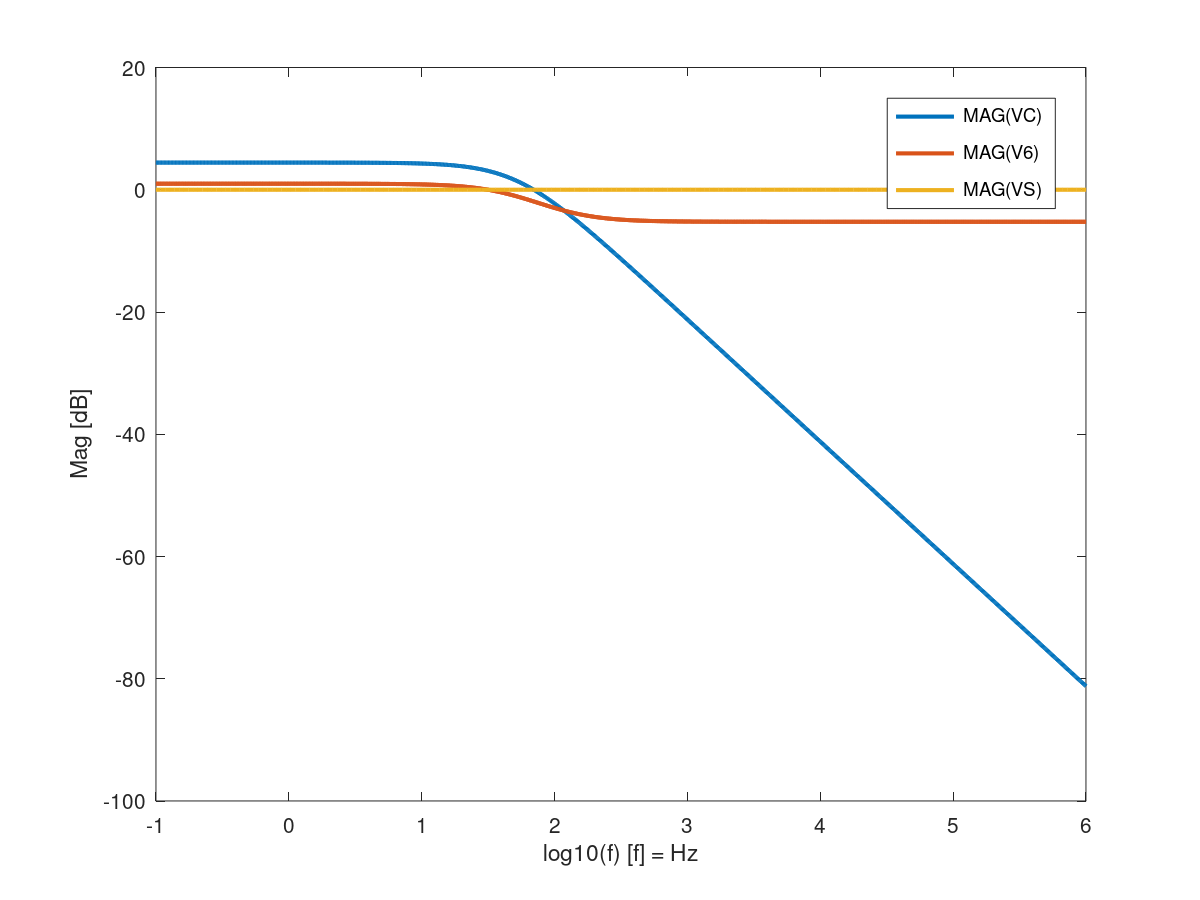
\includegraphics[width = 0.85\linewidth]{../mat/vcmag.png}
        \caption{\textit{Plot of the magnitude in function of the frequency. The frequency is presented in a logarithmic scale, as is the magnitude, which is in dB.}}
    \label{fig:magnitude}
\end{figure}

With amplitude $1$, $V_s$ has a constant magnitude for any frequency as expected, contrary to the other amplitudes that decrease with the increase in frequency, and for really high oscillation in the source, the amplitude of the oscillation in node 6 is practically 0. The critical frequency seems to be at $80Hz$.
\section{Simulation Analysis}

To be sure of the values obtained in \ref{sec:theo}, we made use of Ngspice, a more stable version of the Berkeley SPICE, which is an "open source spice simulator for electric and electronic circuits", as stated in \cite{ngsite}. The code used was the following, \\

{\itshape
TCFELab1 \par
.options savecurrents \\\par

Vin 1 4 5.03847501972 \par
Id 0 6 1.01674167773m \par

$V_{dumb}$ CFP1 7 0 \\\par

R1 2 1 1.03994439216k \par
R2 3 2 2.07923431764k \par
R3 2 5 3.06168544529k \par
R4 4 5 4.09516986362k \par
R5 5 6 3.00136467001k \par
R6 4 CFP1 2.03324628446k \par
R7 7 0 1.02216788331k \\\par

Gb 6 3 2 5 7.01505323139m \par
Hc 5 0 $V_{dumb}$ 8.37372457746k \\\par

.op\par
.control\par
    run\par
    print all\par
.endc\par
.end
}

\vspace{10px}
The first line of this code is the title of the simulation itself, which is followed by the option to save currents, a command that allows the program to, when printing all the variables, also print the currents flowing in every component of the circuit. Then, \textit{Vin} and \textit{Id} are the $V_a$, $I_d$ corresponding to what is shown in Fig. \ref{fig:nodal_scheme}. $V_{dumb}$ is a dumb voltage source that was introduced for a specific reason that will be later explained. In this simulation, we chose node 8 to be GND, which, by Ngspice standards, has to be named node 0.\\

After this, all the resistances were declared in the form \textit{R<name> <n+> <n-> <value>}, where n+ and n- mean the positive and negative nodes of the electronic component, according to the schematics shown in Fig.\ref{fig:polos}. \\

\begin{figure}[h]
    \centering
    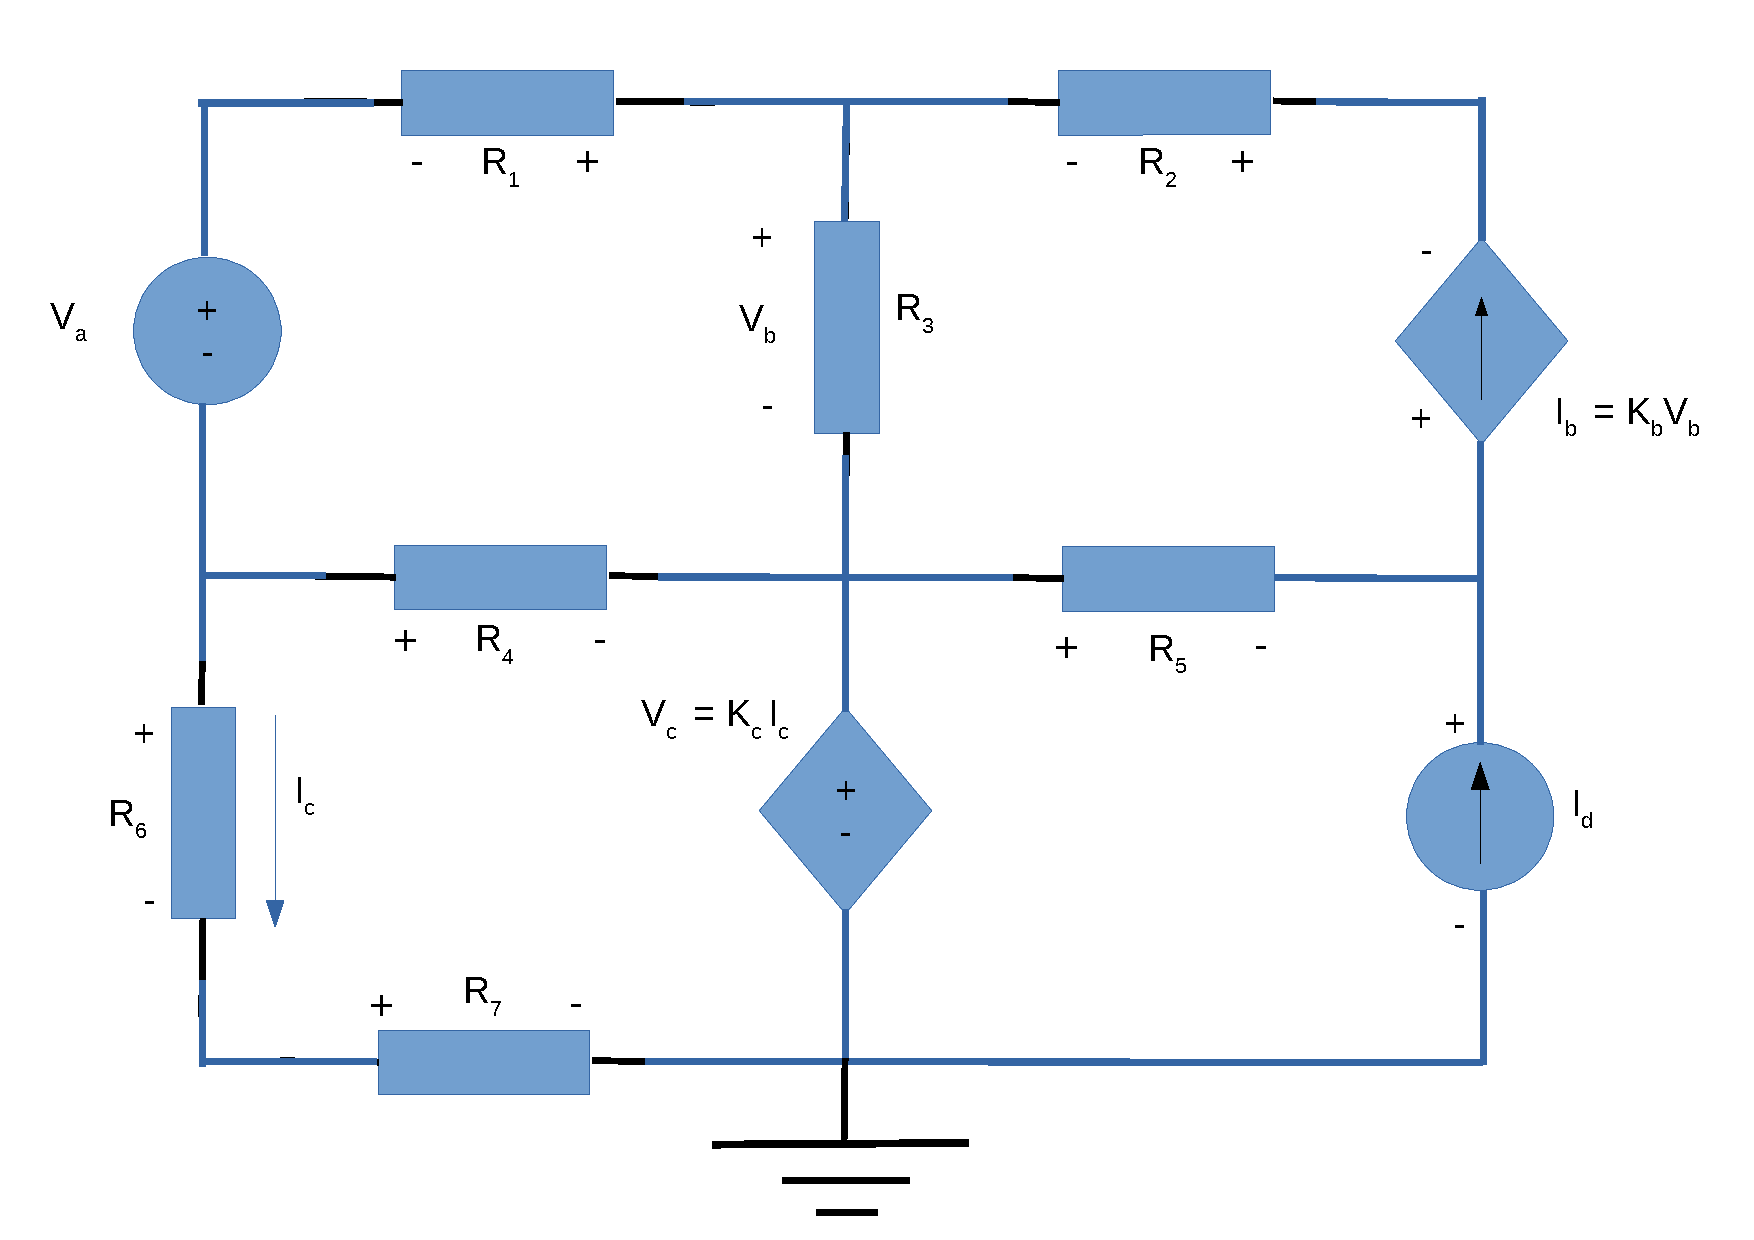
\includegraphics[width = 0.7\linewidth]{esquemacpolos.pdf}
        \caption{\textit{Representation of the convention used to the Ngspice simulation. In the figure above, one can see the conventioned positive and negative terminal for each branch}}
    \label{fig:polos}
\end{figure}

Afterwards, $Gb$ and $Hc$ stand for the voltage-controlled current source $I_b$ and current-controlled voltage source $V_c$ respectively. The first two parameters received by $Gb$ are its positive and negative nodes as expected and then the two nodes where it should calculate the corresponding potential. For $Hc$, the third parameter is $V_{dumb}$ which, as promised, is a voltage source that was introduced for the single purpose that current-controlled voltage sources in \textit{Ngspice} take as a third parameter only voltage sources through which the current in question is flowing through. Thus, because the purpose is to retrieve $I_c$, a dumb voltage source was added after $R_6$, creating a new node that was called CFTP1, which is where $R_6$ then connects. To not alter the circuit at all, the actual induced voltage by $V_{dumb}$ is 0V, thus CFTP1 and node 7 are in short circuit, i.e., the circuit does not "see" $V_{dumb}$. At last, inside \textit{control}, the simulation is ran and everything is printed out, giving the following output:\\\par


\begin{table}[H]
\setlength{\tabcolsep}{10pt}
\renewcommand{\arraystretch}{1.1}
\centering
    \begin{tabular}{||c|c||}
    \hline
    Name & Current/Voltage [A/V]\\
    \hline
    @cb[i] & 0.000000e+00\\ \hline
@ce[i] & 0.000000e+00\\ \hline
@q1[ib] & 7.022567e-05\\ \hline
@q1[ic] & 1.404513e-02\\ \hline
@q1[ie] & -1.41154e-02\\ \hline
@q1[is] & 5.765392e-12\\ \hline
@rc[i] & 1.411536e-02\\ \hline
@re[i] & 1.411536e-02\\ \hline
@rf[i] & 7.022567e-05\\ \hline
@rs[i] & 0.000000e+00\\ \hline
v(1) & 0.000000e+00\\ \hline
v(2) & 0.000000e+00\\ \hline
base & 2.254108e+00\\ \hline
coll & 5.765392e+00\\ \hline
emit & 1.411536e+00\\ \hline
vcc & 1.000000e+01\\ \hline

    \end{tabular}
\vspace{0.2 cm}
\caption{Values for several variables declared in the .net file.}
\label{max}
\end{table}


\vspace{10px}

The values obtained were expected in some way given the results obtained in the theoretical analysis and that were presented in the last section. The reader can check the results knowing that $V_b = V_2 -V_5$ and $V_c = V_5$.\\

However, due to \textit{machine epsilons} and related things, some decimal places might be a bit different. The main cause of this is that Ngspice also uses, whenever possible, nodal analysis. Thus, for solving matrix \ref{eqnodos}, one has to be aware that inverting a 9x9 or 7x7 matrix will introduce a significant margin of error, which explains a possible observable difference in the results obtained, specially between this simulation and the mesh analysis.

\section{Side by side comparison between analysis results}
\label{sec:sidebyside}

\begin{table}[H]
    \begin{minipage}{.4\textwidth}
    \begin{table}[H]
    \centering
    \small
    \begin{tabular}{|c|c|c|c|}
          \hline
          Node/Branch & $@(i) [A]/ v [V]$\\
          \hline
          @cb[i] & 0.000000e+00\\ \hline
@ce[i] & 0.000000e+00\\ \hline
@q1[ib] & 7.022567e-05\\ \hline
@q1[ic] & 1.404513e-02\\ \hline
@q1[ie] & -1.41154e-02\\ \hline
@q1[is] & 5.765392e-12\\ \hline
@rc[i] & 1.411536e-02\\ \hline
@re[i] & 1.411536e-02\\ \hline
@rf[i] & 7.022567e-05\\ \hline
@rs[i] & 0.000000e+00\\ \hline
v(1) & 0.000000e+00\\ \hline
v(2) & 0.000000e+00\\ \hline
base & 2.254108e+00\\ \hline
coll & 5.765392e+00\\ \hline
emit & 1.411536e+00\\ \hline
vcc & 1.000000e+01\\ \hline

          \hline
    \end{tabular}
    \caption{Solution from simulation.}
    \label{tab:ngs_tau}
    \end{table}
    \end{minipage}
    \begin{minipage}{.29\textwidth}
      \centering
      \begin{tabular}{c|c}
        \hline
          Branch &  Current (A) \\
          \hline
          \input{"currents_branches_first_alienea.tex"}
          \hline
      \end{tabular}
    \label{tab:current2}
    \caption{Currents from theoretical solution}
    \end{minipage}
    \begin{minipage}{.29\textwidth}
      \begin{equation} \Vec{b} = \begin{bmatrix}  5.0385\\  4.7582\\  4.1705\\      -0\\  4.7985\\  5.6468\\ -1.8345\\ -2.7568 \end{bmatrix} \label{eqsol} \end{equation}
      \caption{Voltages from theoretical solution}
      \end{minipage}
    \caption{Solution for voltages for all nodes and current for all branches for $t<0$.}
    \end{table}

The only difference found between the 2 solutions, for the digits presetned here are for $V_3$ and $V_6$, but only in the last digit presented, meaning a difference around $10^{-6} V$. Differences that are probably result of numerical errors, rather than real differences in solutions.

\begin{figure}[H]
\hspace{-10mm}
  \subfigure[Theoretical analysis]{% 
    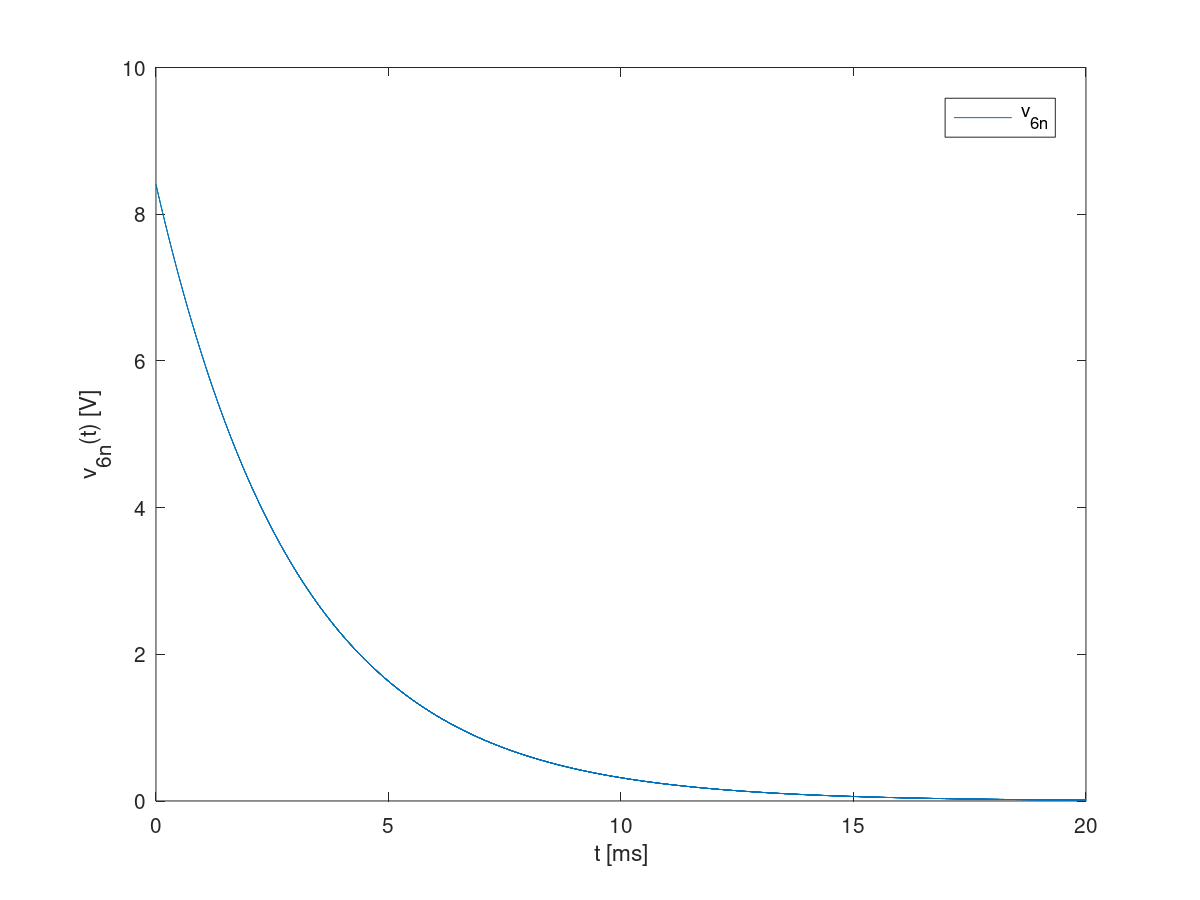
\includegraphics[width=.6\textwidth]{../mat/v6n.png} \label{fig:teo_nat} 
  } 
  \subfigure[Simulation analysis]{% 
    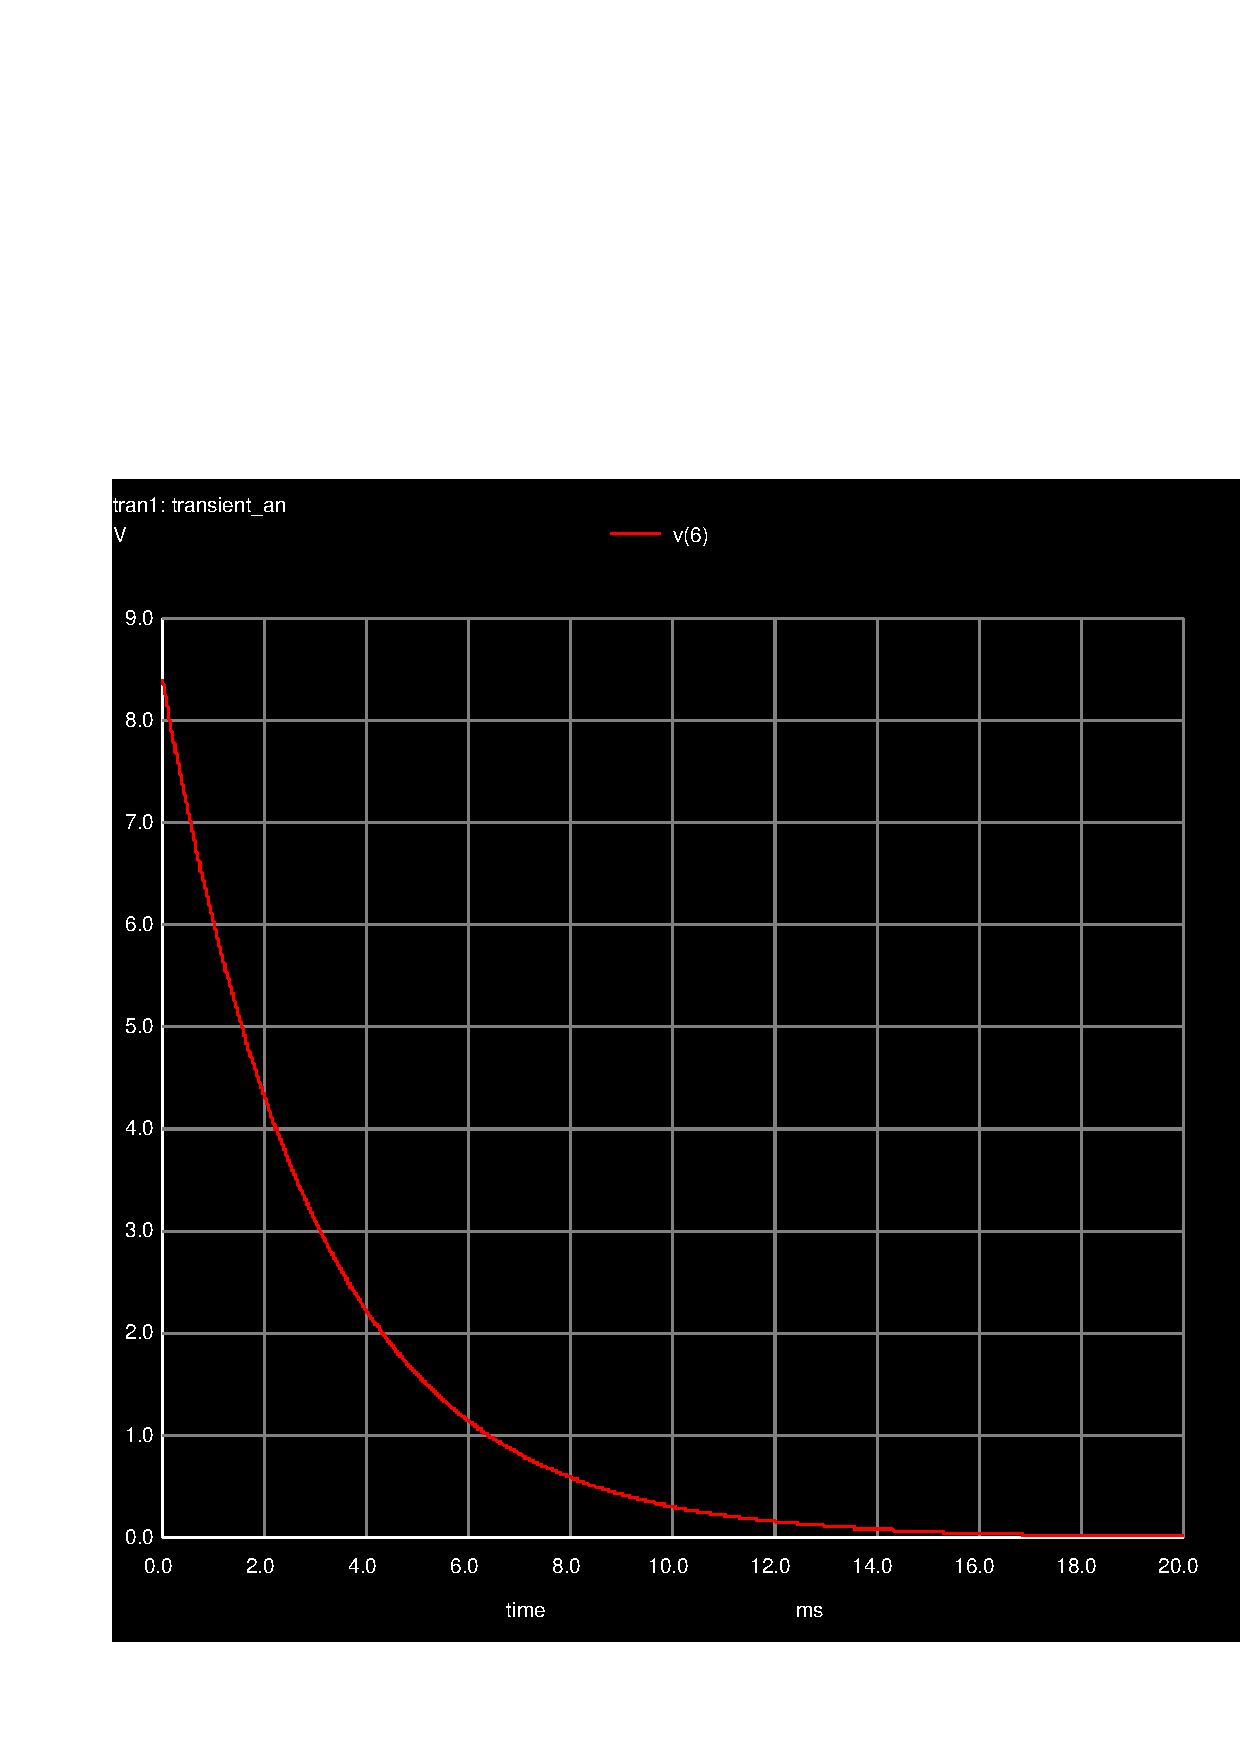
\includegraphics[width=.45\textwidth]{../sim/trans3.pdf} \label{fig:sim_nat} 
  } 
  \caption{Natural solution for voltage in node 6 for $t=[0,20]$.} 
\end{figure}

The solution for the natural solution in node 6 appears to be exactly the same.

\begin{figure}[H]
\hspace{-10mm}
  \subfigure[Theoretical analysis]{% 
    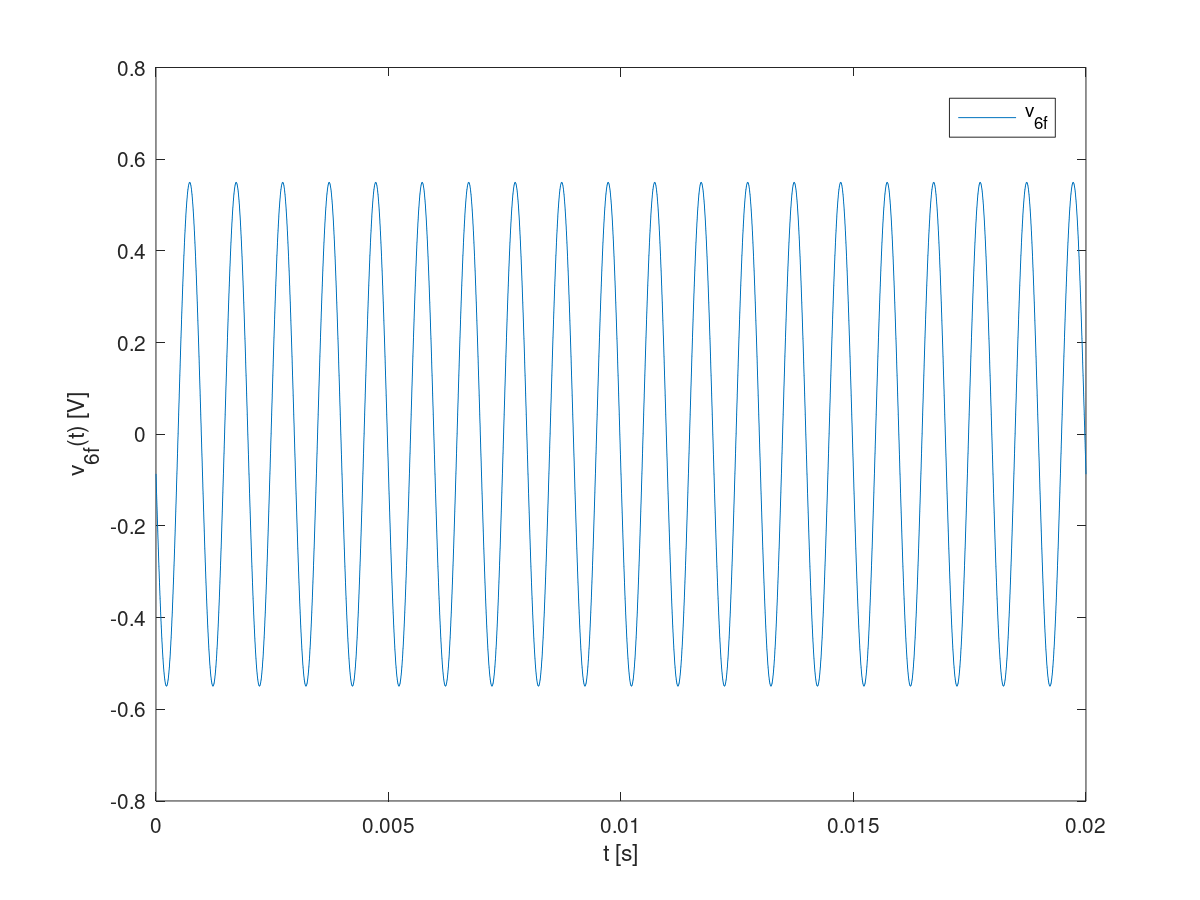
\includegraphics[width=.6\textwidth]{../mat/v6f.png} \label{fig:teo_for} 
  } 
  \subfigure[Simulation analysis]{% 
    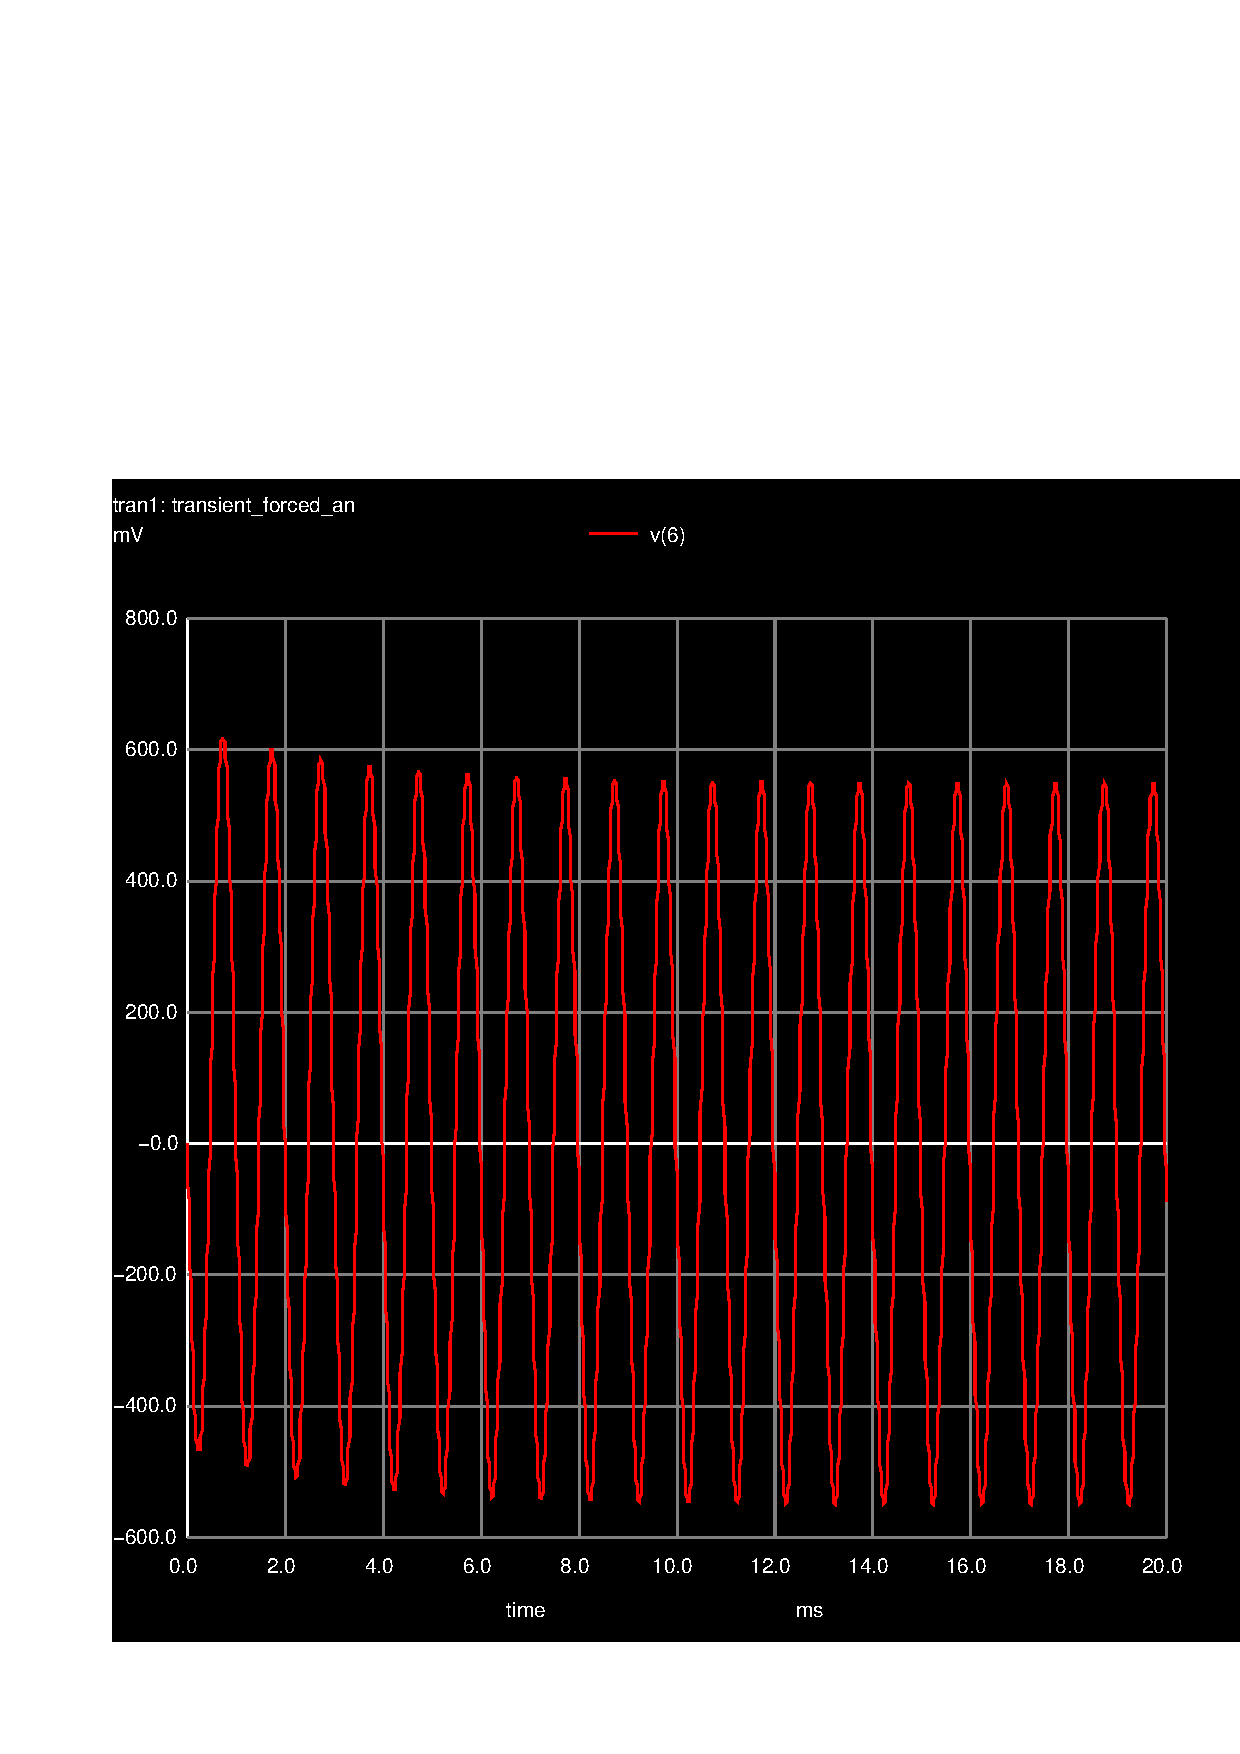
\includegraphics[width=.45\textwidth]{../sim/trans4.pdf} \label{fig:sim_for} 
  } 
  \caption{Forced solution for voltage in node 6 for $t=[0,20]$.} 
\end{figure}

As mentioned before, the only difference found between these 2 solution is that in the forced solution a small offset seems to exist in the first moments of the oscillation, but appears to stabilize on the expected solution.

\begin{figure}[H]
\hspace{-10mm}
  \subfigure[Theoretical analysis]{% 
    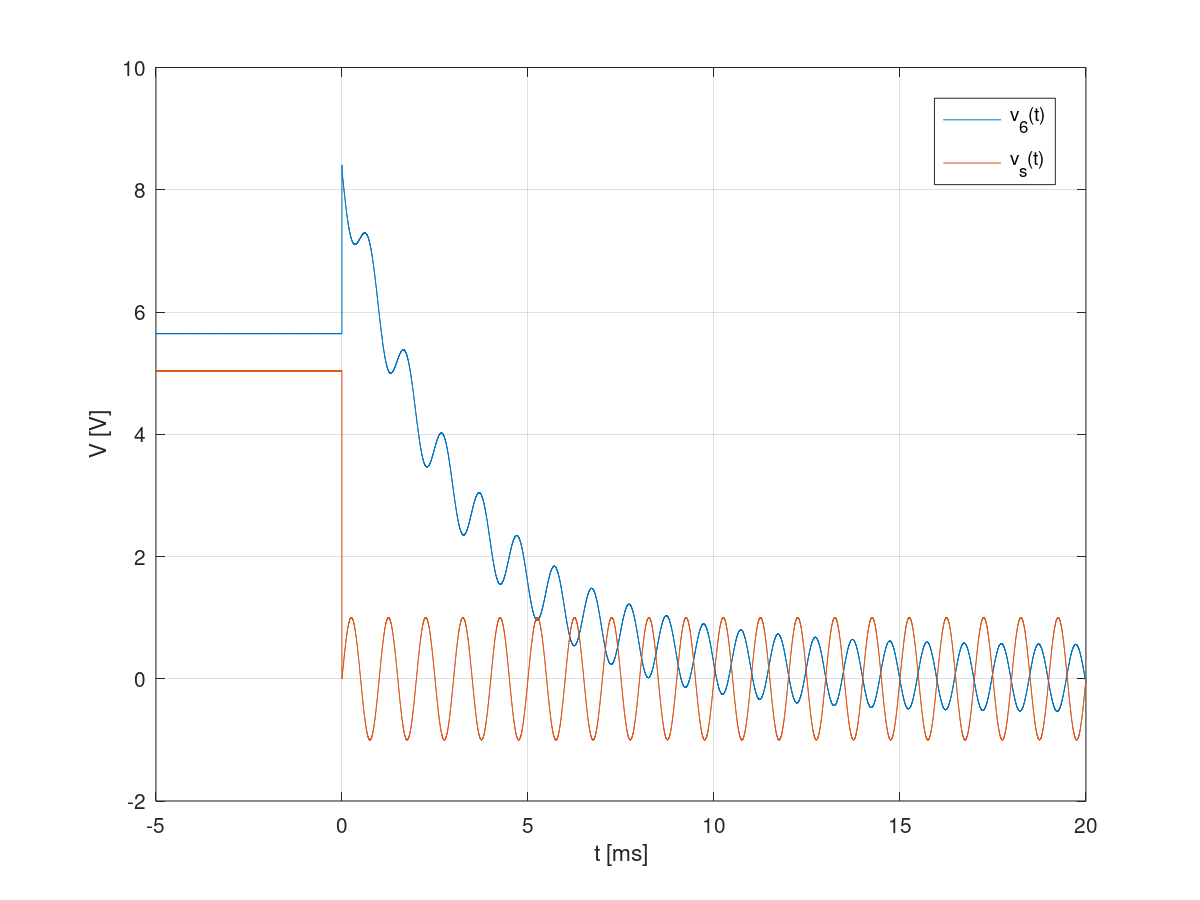
\includegraphics[width=.6\textwidth]{../mat/v6totsze.png} \label{fig:teo_comp} 
  } 
  \subfigure[Simulation analysis]{% 
    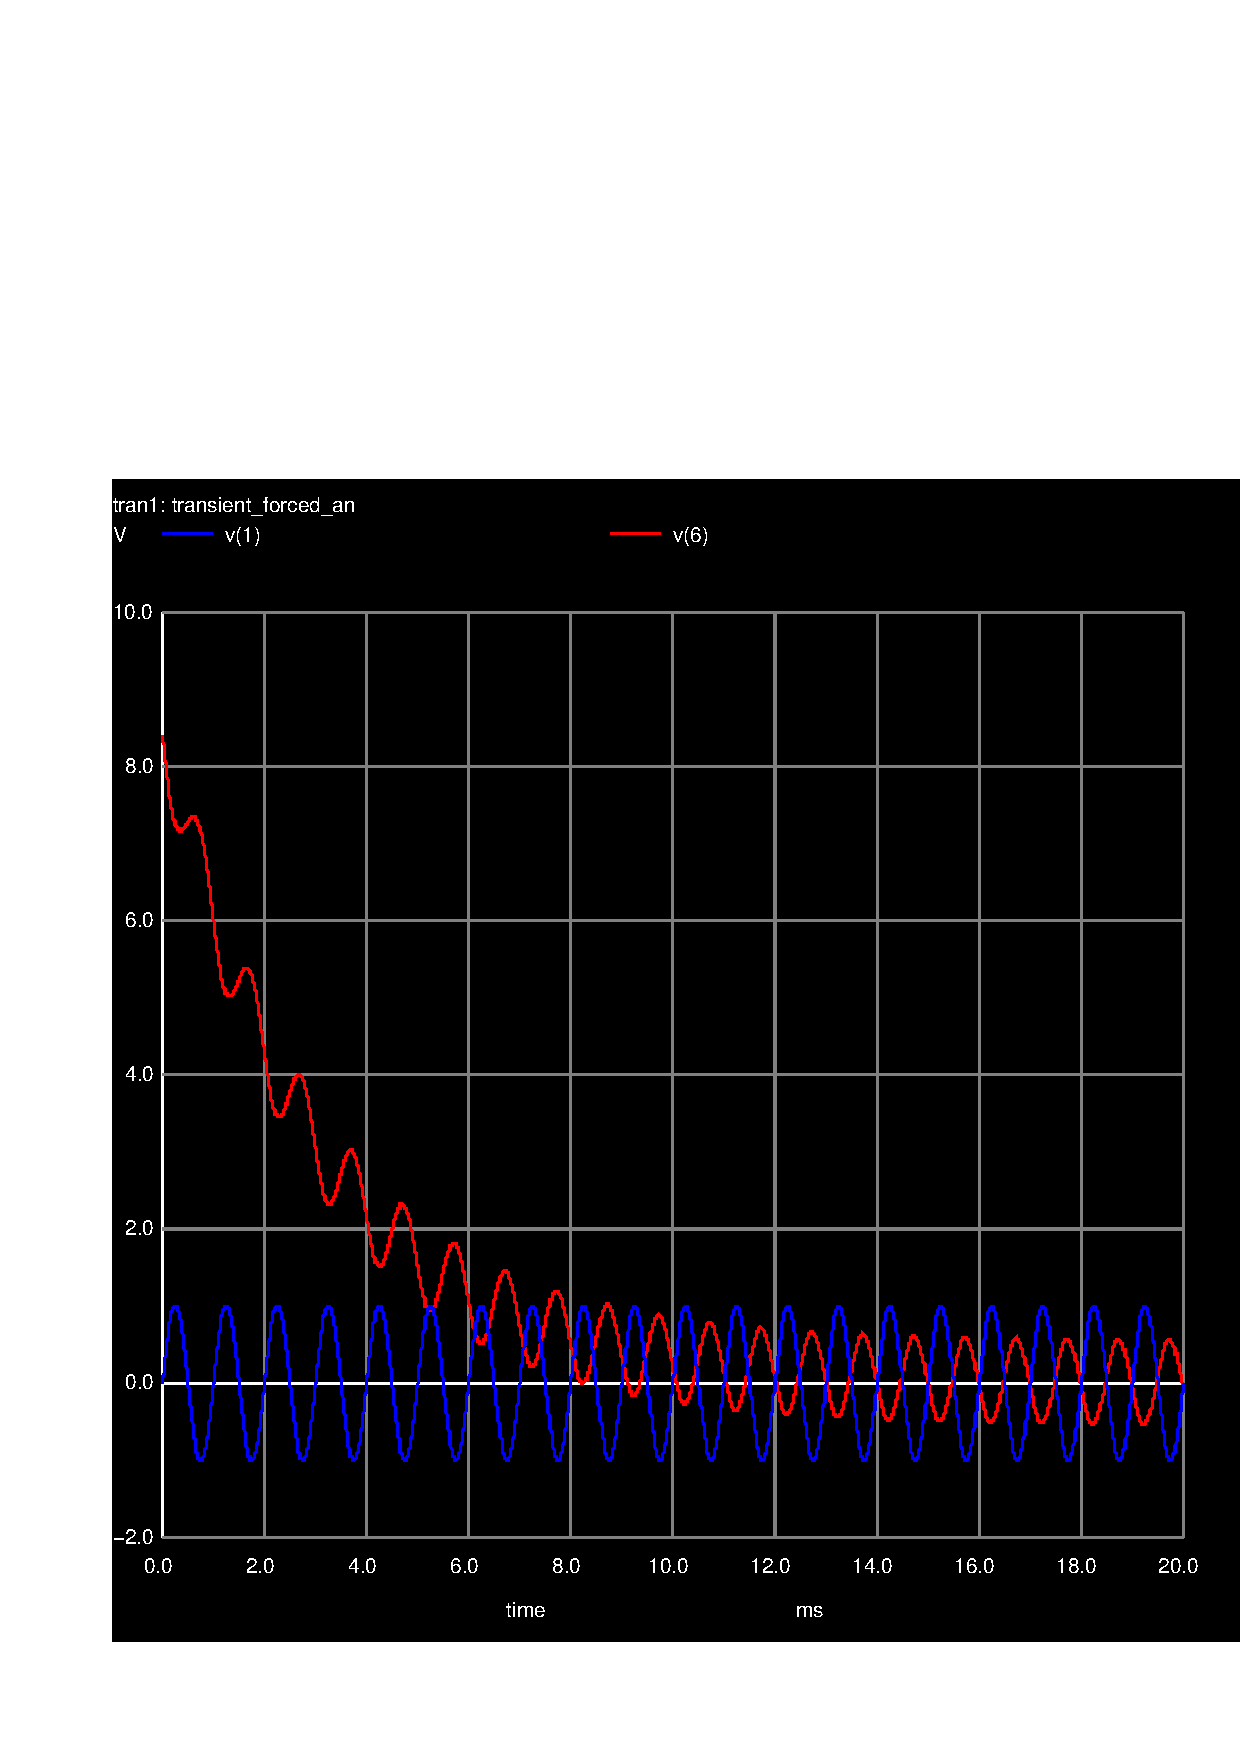
\includegraphics[width=.45\textwidth]{../sim/trans5.pdf} \label{fig:sim_comp} 
  } 
  \caption{Complete solution for voltage in node 6 for $t=[-5,20]$ and $t=[0,20]$.} 
\end{figure}

Besides the part of the forced solution that is now impossible to notice, the plots looks identical even in close inspection.

\begin{figure}[H]
\hspace{-10mm}
  \subfigure[Theoretical analysis]{% 
    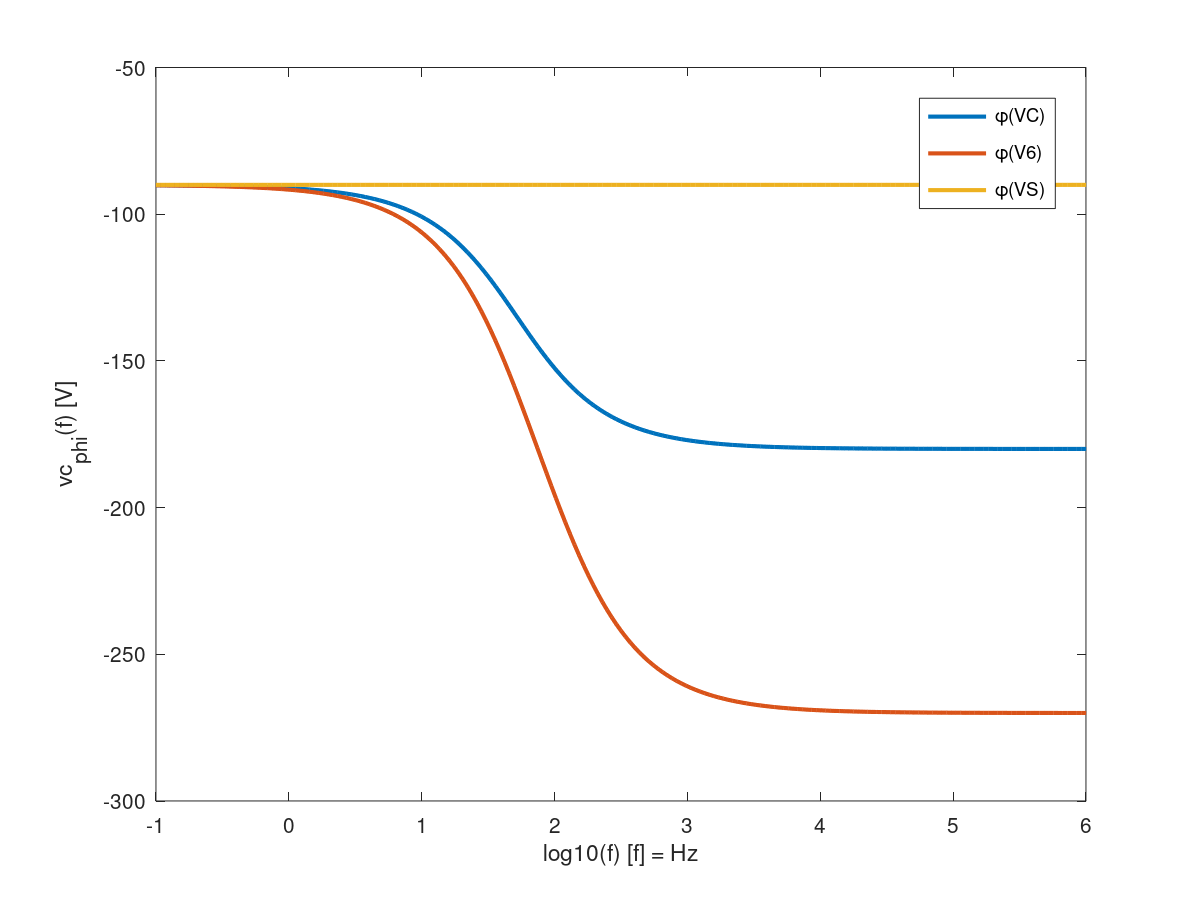
\includegraphics[width=.6\textwidth]{../mat/vcphi.png} \label{fig:teo_phi} 
  } 
  \subfigure[Simulation analysis]{% 
    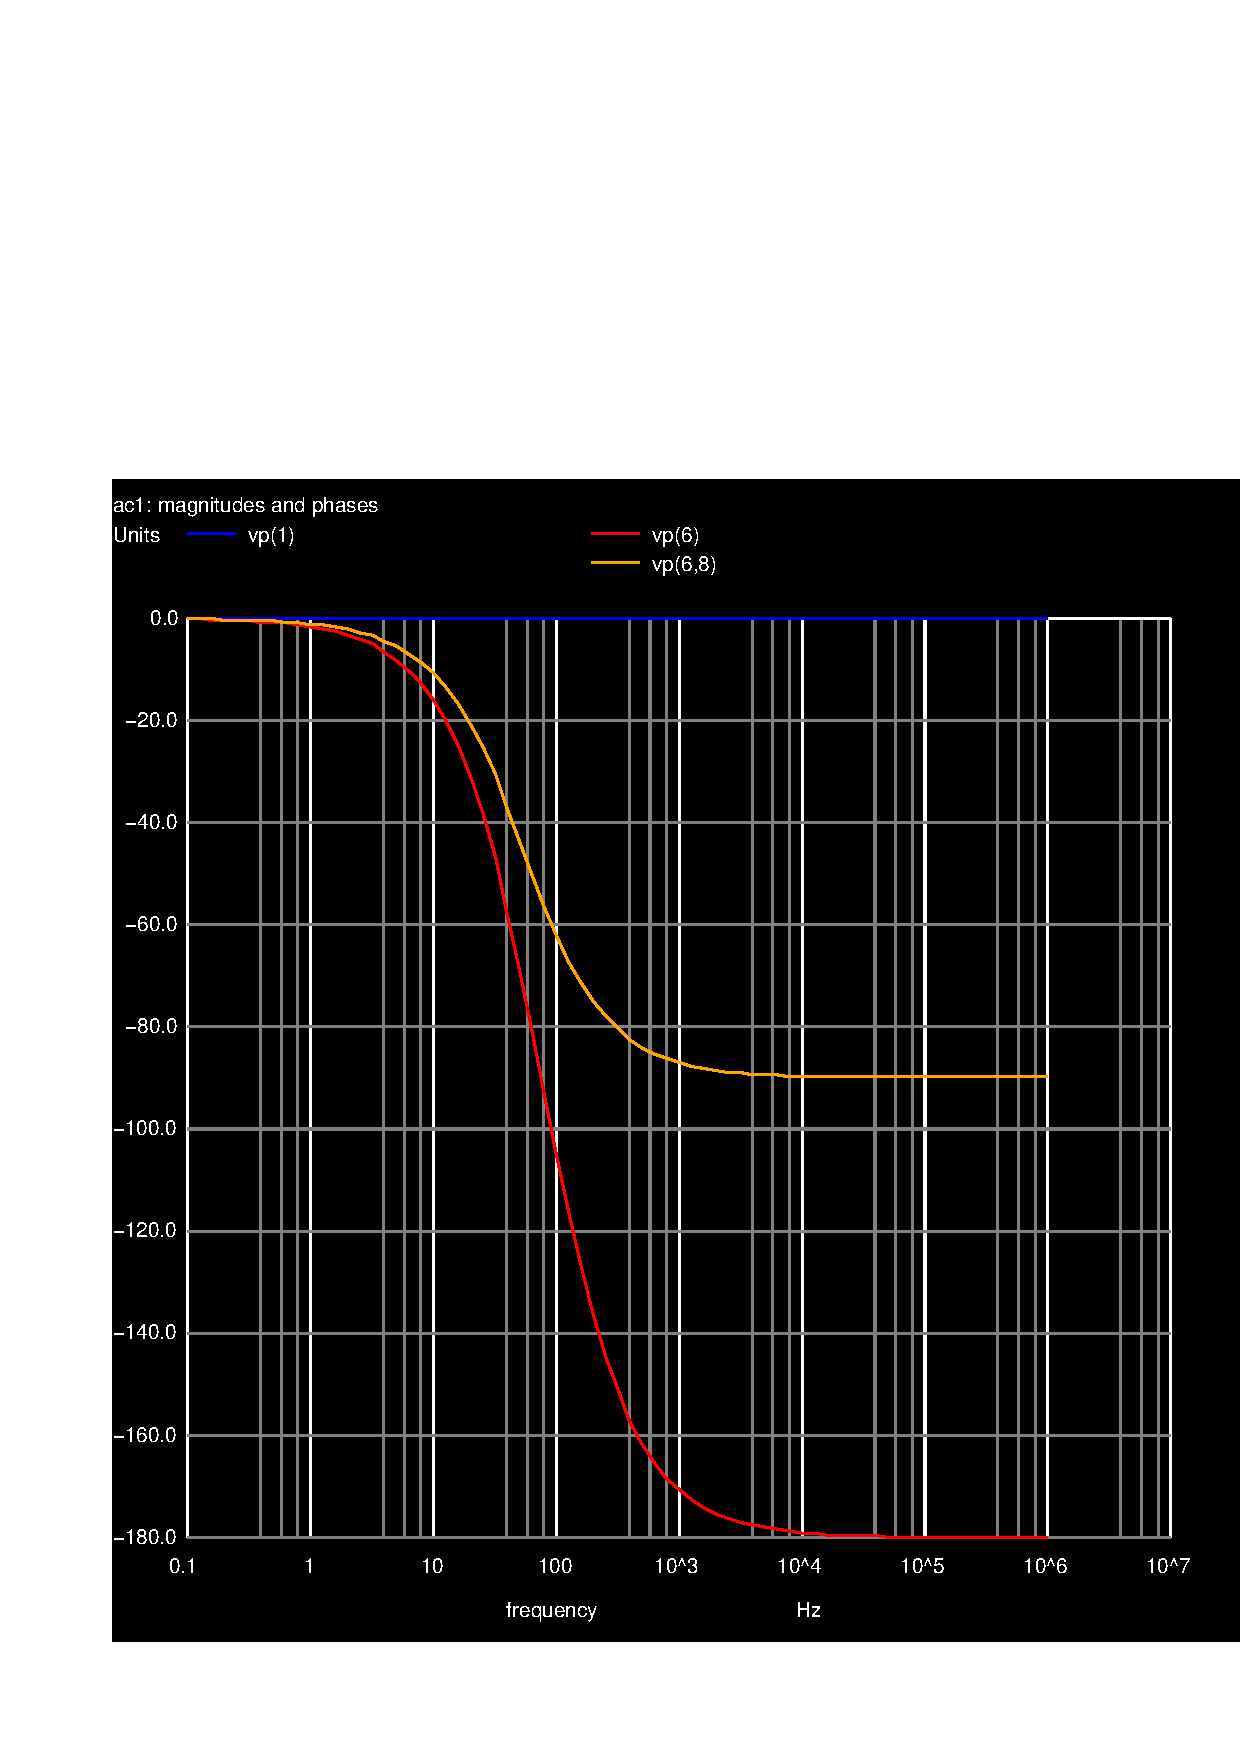
\includegraphics[width=.45\textwidth]{../sim/zezoca.pdf} \label{fig:sim_phi} 
  } 
  \caption{Phase difference as a function of the frequency of the voltage source.} 
\end{figure}

As mentioned before the same transition to a phase difference of a quarter and half a period is seen but \textit{Ngspice} automatically offsets the phases in order for the source to be at 0 degrees.


\begin{figure}[H]
\hspace{-10mm}
  \subfigure[Theoretical analysis]{% 
    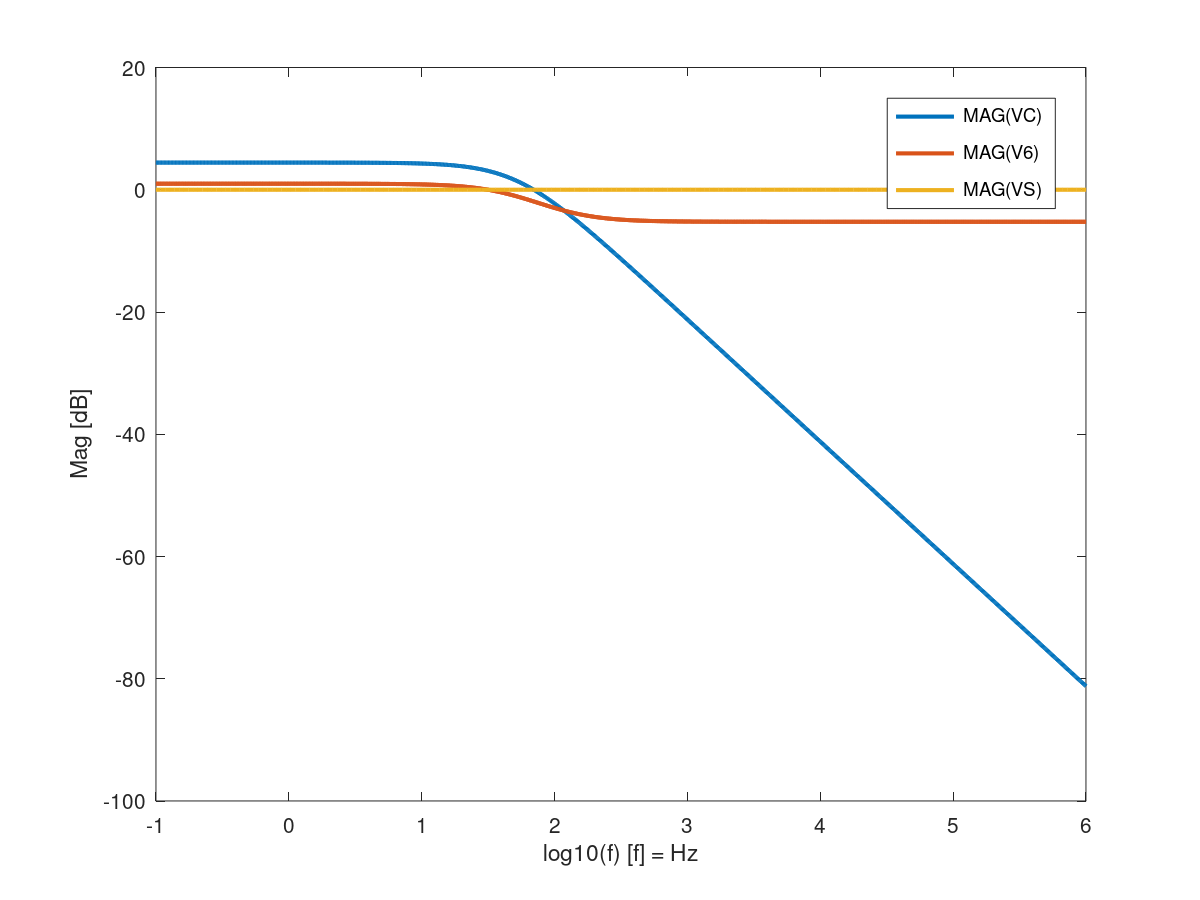
\includegraphics[width=.6\textwidth]{../mat/vcmag.png} \label{fig:teo_mag} 
  } 
  \subfigure[Simulation analysis]{% 
    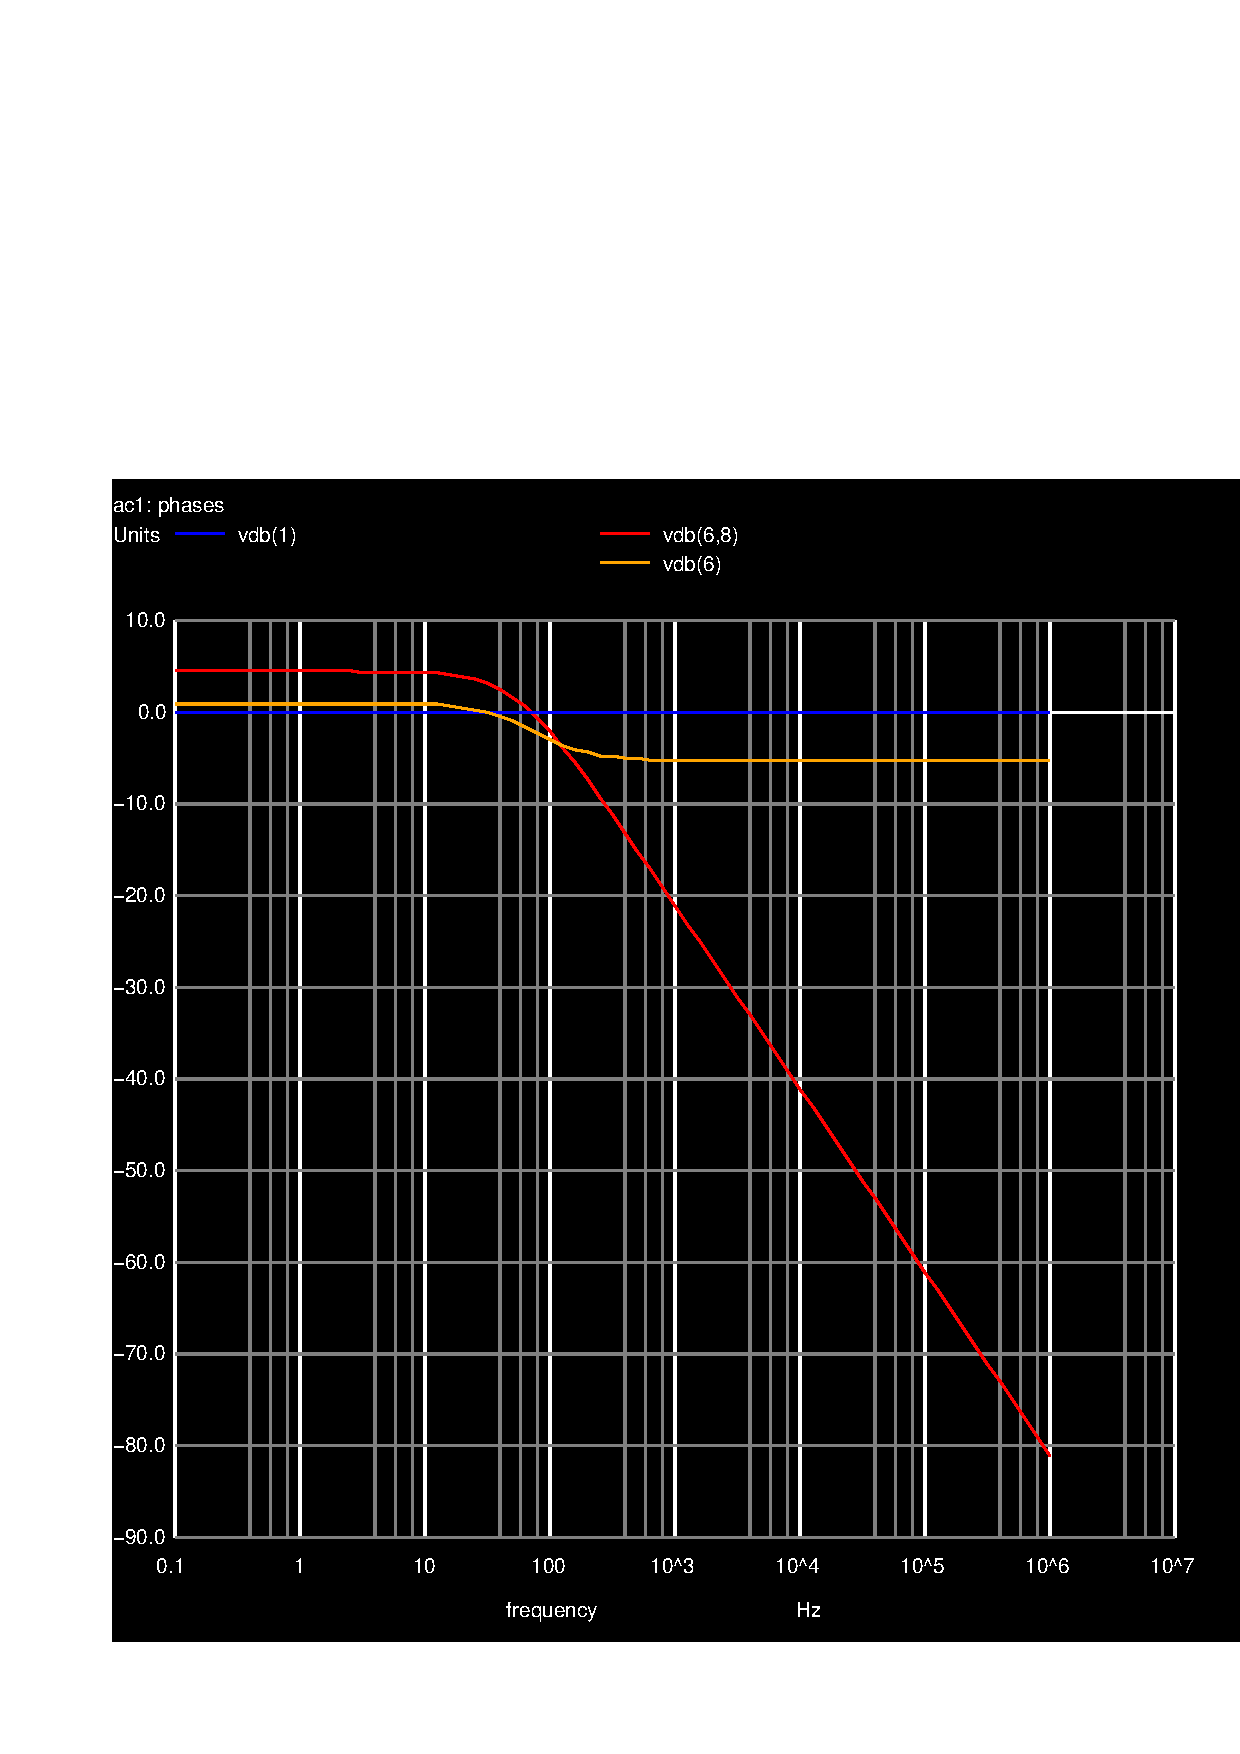
\includegraphics[width=.45\textwidth]{../sim/voltage_mag.pdf} \label{fig:sim_mag} 
  } 
  \caption{Magnitude as a function of the frequency of the voltage source.} 
  Once again no differences can be found between the 2 plots.
  
\end{figure}
\section{Conclusion}
In this laboratory assignment, as presented above, we were proposed to build and study the behaviour of an AC/DC converter. To build it, one used an envelope detector circuit (composed by a full-wave rectifier which turns the AC input into a DC output and a capacitor which smooths the oscillating current) and a voltage regulator circuit (that uses a resistor and multiple diodes which limit the output voltage to the desired value - 12V).\\

To evaluate how good the built converter was, we recurred the merit score presented in \eqref{score}. The results obtained in the simulation analysis (section 2) were very satisfactory except the stabilization time of the circuit, but that wasn't taken into account in the score obtained for the circuit although we had in mind that the circuit shouldn't have a very long stabilization time. The results given by the simulation analysis show an output signal with an average value displaced $\sim 10^{-7}$V from the desired value of 12V and with ripples $\sim 10^{-4}$V. The output voltage obtained is thus almost perfectly equal to the desired output voltage for this converter, which shows that the goal of this simulation was successfully achieved.\\

Comparing the simulation and the theoretical results one can notice a significant difference between the plots and the results obtained with both as anticipated on section 2. In fact, this phenomenon can be justified by the multiple approximations made in the theoretical analysis, namely on the diode model used. In the analysis made using \textit{Octave}, one used the diode models presented in class which neglect the non-linear behaviour of these components which ends up introducing discrepancies between the analysis methods used.\\

However, it is also important to notice that the results obtained on the theoretical analysis were affected of very small ripples, not however as small as in the simulation. To get a better approximation of the merit obtained in the simulation part, we proposed a corrected merit as well, which assumes that the average of the output voltage is exactly $12V$.\\

Therefore, and having explained the differences registered between the theoretical and the simulation analysis, it can be stated that the goals for this laboratory assignment were successfully achieved.
\begin{thebibliography}{9}
\bibitem{ngsite} 
Ngspice official website, \textit{http://ngspice.sourceforge.net/}
\end{thebibliography}


\end{document}
\documentclass[11pt]{article}
\usepackage[utf8]{inputenc}
\usepackage[portuguese, russian, english]{babel}
\usepackage[T1]{fontenc}
\usepackage{subfigure} 
\usepackage{lmodern}
\usepackage{geometry}
\usepackage{authblk}
\usepackage{graphicx}
\usepackage{multicol}
\usepackage{multirow}
\usepackage{float} 
\usepackage{amsmath}

\newcommand\scalemath[2]{\scalebox{#1}{\mbox{\ensuremath{\displaystyle #2}}}}

\geometry{legalpaper, margin=1in}
\renewcommand{\arraystretch}{1.15}

\begin{document}


%%%%%%%%%%%%%%%%%%%%%%%%%%%%%%%%%%%%%%%%%%%%%%%%%%%%%%%%%%%%%%%%%%%%%%%%
%                                                                      %
%     File: Thesis_FrontCover.tex                                      %
%     Tex Master: Thesis.tex                                           %
%                                                                      %
%     Author: Andre C. Marta                                           %
%     Last modified :  2 Jul 2015                                      %
%                                                                      %
%%%%%%%%%%%%%%%%%%%%%%%%%%%%%%%%%%%%%%%%%%%%%%%%%%%%%%%%%%%%%%%%%%%%%%%%

\thispagestyle {empty}

% IST Logo - Signature A
% parameters: bb=llx lly urx ury (bounding box), width=h_length, height=v_length, angle=angle, scale=factor, clip=true/false, draft=true/false. 

\includegraphics[bb=9.5cm 11cm 0cm 0cm,scale=0.29]{IST_A_CMYK_POS}

\begin{center}
%
% Figure (Image or plot)
\vspace{1.0cm}
% height = 50 mm
%\includegraphics[height=50mm]{Figures/Airbus_A350.jpg}

% Title, author and degree
\vspace{1cm}
{\FontLb Circuit Theory and Electronics Fundamentals} \\ % <<<<< EDIT TITLE
\vspace{1cm}
{\FontSn Department of Electrical and Computer Engineering, Técnico, University of Lisbon} \\ % <<<<< EDIT COURSE
\vspace{1cm}
{\FontSn Example Laboratory Report} \\
\vspace{1cm}
{\FontSn February 27, 2021} \\ % <<<<< EDIT DATE (corresponds to date of oral examination)
%
\end{center}


\maketitle

\renewenvironment{abstract}[1]
  {\bigskip\selectlanguage{#1}%
   \begin{center}\bfseries\abstractname\end{center}}
  {\par\bigskip}

\begin{abstract}{english}
    In this report, we show a concise analysis of a 4 single mesh circuit through mesh and nodal analysis. Hitherto Ngspice has been considered a good circuit analyser and thus chosen it was to run the same circuit for comparison with the aforementioned theoretical analysis.
\end{abstract}
\tableofcontents
\addcontentsline{toc}{section}{\listtablename}
\listoftables
\addcontentsline{toc}{section}{\listfigurename}
\listoffigures
\cleardoublepage

\section{Introduction}
The main goal of this laboratory assignment is to design, implement and analyse a band-pass filter (BPF) using an OP-AMP (operational amplifier) having in mind that it should have a good relation efficiency-price. The final objective was to get a central frequency of $1kHz$ for the output signal and a voltage gain of $40dB$ and the circuit's efficiency will be measured considering these objectives that were set. \\

So, in order to evaluate the relation efficiency-price of the built circuit, we will use a merit figure that considers the total cost of the circuit and the deviation to the desired gain and central frequency, defined as:

\begin{equation}
    M = \frac{1}{cost \cdot |40 - gain| \cdot |1000 - central freq.|}
    \label{merit}
\end{equation}

To calculate the total cost associated to this circuit, one considered that it equals the sum of the cost of the resistors, capacitors and transistors which is given by:

\begin{table}[H]
    \centering
    \begin{tabular}{|c|c|}
        \hline
        \textbf{Component} &  \textbf{Price}\\
        \hline
        Resistors & 1 MU $k\Omega^{-1}$ \\ \hline
        Capacitors & 1 MU $\mu F^{-1}$ \\ \hline
        Transistors & 0.1 MU transistor$^{-1}$\\
        \hline
    \end{tabular}
    \caption{Price table for the components used}
    \label{tab:price}
\end{table}

The central frequency represented on eq. \eqref{merit} can be directly calculated from the definition of transfer function for this system and it is given by the geometric mean of the lower and higher cutoff frequencies:

\begin{equation}
    central freq. = \sqrt{f_H f_L}
\end{equation}

in which $f_H$ corresponds to the higher cutoff frequency and $f_L$ to the lower cutoff frequency. Finally, the value for the voltage gain used on eq. \eqref{merit} is easily obtained as the correspondent voltage value for the central frequency obtained. \\

The circuit used to implement this band-pass filter using an OP-AMP can be divided in 3 main regions as it can be seen on Fig. \ref{initialscheme}

\begin{figure}[H]
    \centering
    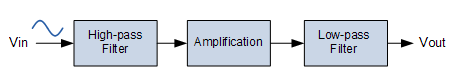
\includegraphics{esquemabunituh.PNG}
    \caption{Simplified scheme to present the 3 regions in which the circuit used can be divided}
    \label{initialscheme}
\end{figure}

The first part, a high-pass filter stage, will essentially have a resistor and a capacitor (i.e. will only pass signals with a frequency higher than a certain cutoff frequency, $f_L$). This part is followed by an amplification unit which will have the main objective of increasing the output voltage gain and which counts with an OP-AMP and two resistors. Finally, one implemented a low-pass filter stage on the circuit which operates on the opposite way of the high-pass filter, i.e. blocks all the signals with a frequency higher than a certain cutoff frequency, $f_H$). \\

As it is trivial, the high-pass filter and the low-pass filter blocking simultaneously frequencies lower than $f_L$ and higher that $f_H$ will act as a band-pass filter as desired. \\

Furthermore, and considering all the points mentioned before, the circuit used for this purpose was the following:


The results were obtained through a theoretical analysis, in which one predicted the output by using a theoretical method that suited the real circuit and through a simulation that was made using \textit{Ngspice}. The results obtained through both methods will be analysed throughout the report. However, because the models used in \textit{Ngspice} are more correct than the ones used on the theoretical analysis, any type of optimization was done almost exclusively in the simulation analysis.\\
\section{Theoretical Analysis}
\label{sec:theo}
\subsection{Nodal Analysis at $t<0$}
\label{sec:1st}
First of all, one can start by applying the nodal analysis method at $t<0$ to find the voltages of all nodes and, afterwards, using Ohm's law, the currents that flow through each branch of the circuit. Note that the labels used to refer to each node and branch are exactly the same as presented in Fig. \ref{fig:bigscheme}.

So, the next step is to write linearly indepedent equations that will allow us to get the voltages at each node. Note that for $t<0$, we will have $u(t) = 0 \Longrightarrow I_c = 0$ and so, by applying the condition associated with the independent voltage source, one will have a constant value for $v_s(t)$, such that $v_s (t) = V_s$ for $t<0$ (as it can be seen in the expression for the independent voltage source in Fig. \ref{fig:bigscheme}.

\begin{equation}
    \begin{cases}
        V_1 - V_4 = V_s \hspace{15px} \text{(independent voltage source)}\\
        (V_2-V_1)G_1 + (V_2-V_3)G_2 + (V_2-V_5)G_3 = 0 \hspace{15px}\text{(node 2)}\\
        (V_3 - V_2)G_2 + (V_5 - V_2)K_b = 0 \hspace{15px}\text{(node 3)}\\ 
        V_4 = 0 \hspace{15px}\text{(node 4 assigned to GND)}\\
        (V_5-V_2)G_3 + (V_5-V_4)G_4 + (V_5-V_6)G_5 + (V_8-V_7)G_7 = 0 \hspace{15px}\text{(supernodal equation)}\\
        (V_6-V_5)G_5 + (V_2-V_5)K_b = 0 \hspace{15px}\text{(node 6)}\\
        (V_7-V_4)G_6 + (V_7-V_8)G_7 = 0 \hspace{15px}\text{(node 7)}\\
        V_5 - V_8 = (V_7-V_4)K_dG_6 \hspace{15px}\text{(restriction equation involving dependent voltage source)}
    \end{cases}
\end{equation}

Note that the last equation of this system, the restriction equation involving the current-controlled voltage source, urges as the result of the combination of two equations. As shown in Fig. \ref{fig:bigscheme}, one can write $V_d$ as:

\begin{equation}
    V_d = K_d I_d
\end{equation}

and also:

\begin{equation}
    V_d = V_5 - V_8
\end{equation}

Because $I_d$ is the current which flows through the resistor $R_6$ (one could write an equivalent equation by using the resistor $R_7$, as the current flowing through it is exactly the same), one can easily write, using Ohm's Law:

\begin{equation}
    I_d = (V_7 - V_4)G_6
\end{equation}

Combining these 3 equations, one can obtain the restriction equation used in the previous system:

\begin{equation}
    V_d = V_5 - V_8 = (V_7 - V_4)G_6 K_d
\end{equation}

Converting this system of equations to its matricial form, one can obtain:

\begin{equation}
    \begin{bmatrix}
     1 &  0      &  0 &    -1  &     0      &  0  &  0    &  0\\
     -G_1 & G_1+G_2+G_3 & -G_2  & 0   &  -G_3       &  0  &  0    &  0\\
     0   & -G_2-K_b    & G_2  & 0   &   K_b       &  0  &  0    &  0\\
     0   & 0        & 0   & 1 & 0       &  0  & 0   & 0\\
     0   & -G_3      &  0 &  -G_4  &   G_3+G_4+G_5 & -G_5 &  -G_7    & G_7\\
     0   & K_b       & 0  &  0    & -G_5-K_b     & G_5  & 0     & 0\\
     0   & 0        & 0  & -G_6   &  0         & 0   & G_6+G_7 & -G_7\\
     0   & 0        & 0  &  -K_dG_6    &  1         & 0   & K_dG_6     & -1
    \end{bmatrix} 
    \begin{bmatrix}
        V_1\\
        V_2\\
        V_3\\
        V_4\\
        V_5\\
        V_6\\
        V_7\\
        V_8
    \end{bmatrix}
    = 
    \begin{bmatrix}
        V_s\\
        0\\
        0\\
        0\\
        0\\
        0\\
        0\\
        0
    \end{bmatrix}
\label{eqnodos2}
\end{equation}

The matrix system \ref{eqnodos2} is composed of a very sparse matrix, thus we also advise for using correspondingly adapted sparse matrix solvers if possible, but this is already out of the scope of this discipline and laboratory. Getting back to the point, the solution to the matrix system is,

%V1 & 5.038475019720000E+00  \\ \hline
V2 & 4.758223649291032E+00 \\ \hline
V3 & 4.170534768621250E+00 \\ \hline
V5 & 4.798515115188197E+00 \\ \hline
V6 & 5.646841168887640E+00  \\ \hline
V7 & -1.834523049106916E+00 \\ \hline
V8 & -2.756787388808905E+00 \\ \hline


Finally, to find the currents in the circuit, one can apply Ohm's law as one knows all the resistor values and the voltages in all of the circuit's nodes (presented in \eqref{eqsol}. \\

Labeling the positive and negative terminals of each component as inserted in \textit{Ngspice}, and as it can be seen in Fig. something, one can obtain

\begin{table}[H]
    \begin{minipage}{.5\textwidth}
      \begin{equation} \Vec{b} = \begin{bmatrix}  5.0385\\  4.7582\\  4.1705\\      -0\\  4.7985\\  5.6468\\ -1.8345\\ -2.7568 \end{bmatrix} \label{eqsol} \end{equation}
    \end{minipage}
    \begin{minipage}{.5\textwidth}
      \centering
      \begin{tabular}{c|c}
        \hline
          Branch &  Current (A) \\
          \hline
          I(R1) & -0.000269\\
I(R2) & 0.000283\\
I(R3) & -0.000013\\
I(R4) & -0.001172\\
I(R5) & -0.000283\\
I(R6) & 0.000902\\
I(R7) & 0.000902\\
I(Vs) & -0.000269\\
I(Vd) & -0.000902\\
Id  & 0.000902\\
Ib & -0.000283\\
Ic & 0.000000\\

          \hline
      \end{tabular}
    \end{minipage}
    \caption{Theoretical solution for voltages for all nodes and current for all branches for $t<0$.}
    \label{tab:current}
\end{table}


\subsection{$R_{eq}$ and time constant $\tau$}
Next up, we need to determine the equivalent resistance, $R_eq$, as seen from the capacitor terminals to find the time constant associated with this circuit, $\tau = R_{eq}C$, so that one can analyse, afterwards, the natural and the forced solution of the circuit. \\

To do that, one can start by "shutting down" the independent voltage source of the circuit, $V_s$, by making it $V_s = 0$, i.e., replacing it by a short circuit. Afterward, as we want to calculate $R_{eq}$ as seen by the terminals of the capacitor, one should now substitute the capacitor by a voltage source with value $V_x = V_6 - V_8$, where one can use the values obtained in section \ref{sec:1st} for $V_6$ and $V_8$. This whole process is adopted because the value $R_{eq}$ which we are seeking is nothing more than the Thévenin Resistance, $R_{th}$, of the circuit as seen by the terminals of the capacitor. \\

Rewriting the system of equations with this new constraints (knowing the value for $V_x$ and imposing $V_s = 0$), one can write the system as:

\begin{equation}
    \begin{bmatrix}
     1 &  0      &  0 &    -1  &     0      &  0  &  0    &  0\\
     -G_1 & G_1+G_2+G_3 & -G_2  & 0   &  -G_3       &  0  &  0    &  0\\
     0   & -G_2-K_b    & G_2  & 0   &   K_b       &  0  &  0    &  0\\
     0   & 0        & 0   & 1 & 0       &  0  & 0   & 0\\
     0   & -G_3+K_b      &  0 &  -G_4  &   G_3+G_4-K_b & 0 &  -G_7    & G_7\\
     0   & 0       & 0  &  0    & 0     & 1  & 0     & -1\\
     0   & 0        & 0  & -G_6   &  0         & 0   & G_6+G_7 & -G_7\\
     0   & 0        & 0  &  -K_dG_6    &  1         & 0   & K_dG_6     & -1
    \end{bmatrix} 
    \begin{bmatrix}
        V_1\\
        V_2\\
        V_3\\
        V_4\\
        V_5\\
        V_6\\
        V_7\\
        V_8
    \end{bmatrix}
    = 
    \begin{bmatrix}
        0\\
        0\\
        0\\
        0\\
        0\\
        V_x\\
        0\\
        0
    \end{bmatrix}
\label{eqnodos}
\end{equation}

Which take us to this result:

\begin{equation}
    \begin{bmatrix}
        V_1\\
        V_2\\
        V_3\\
        V_4\\
        V_5\\
        V_6\\
        V_7\\
        V_8
    \end{bmatrix}
    = 
    \begin{bmatrix}
        0\\
        0\\
        0\\
        0\\
        0\\
        8.40363\\
        0\\
        0
    \end{bmatrix}V
\end{equation}

Now that one obtained the values for every node voltage, and having in mind that $I_x$ can be written as $I_x = -(I_b+I_5)$:

\begin{equation}
\begin{cases}
    I_b = K_b(V_2 - V_5) = 0mA\\
    I_5 = (V_6 - V_8)G_5 \approx -2.80 mA
\end{cases}
    \Longrightarrow I_x = -I_5 = 2.80 mA
\end{equation}

Now that one obtained the values of $V_x$ and $I_x$, one can finally obtain the value for $R_eq$, which can be written as:

\begin{equation}
    R_{eq} = \frac{V_x}{I_x} \approx 3.0014 k\Omega
\end{equation}

Finally, as for RC circuits, the time constant can be expressed as:

\begin{equation}
    \tau = R_{eq}
\end{equation}

one can obtain that for this specific circuit, $tau$ can be written as:

\begin{equation}
    \tau \approx 3.0516 ms
\end{equation}
\subsection{Node analysis for $t\geq0$ - natural solution for $v_6(t)$}
Analysing now the circuit in $t>0$ in order to determine the evolution of the voltage on node 6, $V_6$, with time, $v_6(t)$, one can start by determining its natural solution. To do that, we start by assuming the general form of this solution which can be written as:

\begin{equation}
    v_{6n}(t) = v_{6n} (t\to\infty) + (v_{6n}(t = 0) - v_{6n}(t\to\infty))e^{-\frac{t}{\tau}}
\label{generalfor}
\end{equation}

in which $\tau$ represents the time constant for this RC circuit, i.e., $\tau = R_{eq}C$, as calculated on the previous section.\\

Starting by $v_6 (t=0)$, the initial condition for the solution which we are seeking is $V_x$, the voltage obtained in the last section for the voltage source by which one replaced the capacitor. So on, using the last section results, as $V_x = V_6 - V_8$ and $V_8 = 0$, one can infer that $V_x = V_6$, and so one can conclude that $v_6(t=0) = V_x$. \\

Only $v_(t\to\infty)$ remains unknows. To find it, one can run again the nodal analysis system of equations with $V_s = 0$, as we are searching only for the natural solution by now. So, one can write the equivalent matricial equation for $t\to\infty$ as:

\begin{equation}
    \begin{bmatrix}
     1 &  0      &  0 &    -1  &     0      &  0  &  0    &  0\\
     -G_1 & G_1+G_2+G_3 & -G_2  & 0   &  -G_3       &  0  &  0    &  0\\
     0   & -G_2-K_b    & G_2  & 0   &   K_b       &  0  &  0    &  0\\
     0   & 0        & 0   & 1 & 0       &  0  & 0   & 0\\
     0   & -G_3+K_b      &  0 &  -G_4  &   G_3+G_4-K_b & 0 &  -G_7    & G_7\\
     0   & 0       & 0  &  0    & 0     & 1  & 0     & -1\\
     0   & K_b        & 0  & 0   &  -G_5-K_b         & G_5   & 0 & 0\\
     0   & 0        & 0  &  -K_dG_6    &  1         & 0   & K_dG_6     & -1
    \end{bmatrix} 
    \begin{bmatrix}
        V_1\\
        V_2\\
        V_3\\
        V_4\\
        V_5\\
        V_6\\
        V_7\\
        V_8
    \end{bmatrix}
    = 
    \begin{bmatrix}
        0\\
        0\\
        0\\
        0\\
        0\\
        0\\
        0\\
        0
    \end{bmatrix}
\label{eqnodos}
\end{equation}

which results in the following solution:

\begin{equation}
    \begin{bmatrix}
        V_1\\
        V_2\\
        V_3\\
        V_4\\
        V_5\\
        V_6\\
        V_7\\
        V_8
    \end{bmatrix}
    = 
    \begin{bmatrix}
        0\\
        0\\
        0\\
        0\\
        0\\
        0\\
        0\\
        0
    \end{bmatrix} V
\label{zeros}
\end{equation}

Knowing $v_{6n}(t = 0)$ and $v_{6n}(t\to\infty)$ one can now use equation \eqref{generalfor} to find the expression for the natural solution of the voltage on node 6:

\begin{equation}
    v_{6n}(t) \approx 8.4036e^{-\frac{t}{0.0030516}}
\end{equation}

Plotting the function obtained on the interval $t \in [0,20]ms$, one can get the graph shown in Fig. \ref{fig:natural}

\begin{figure}[H]
    \centering
    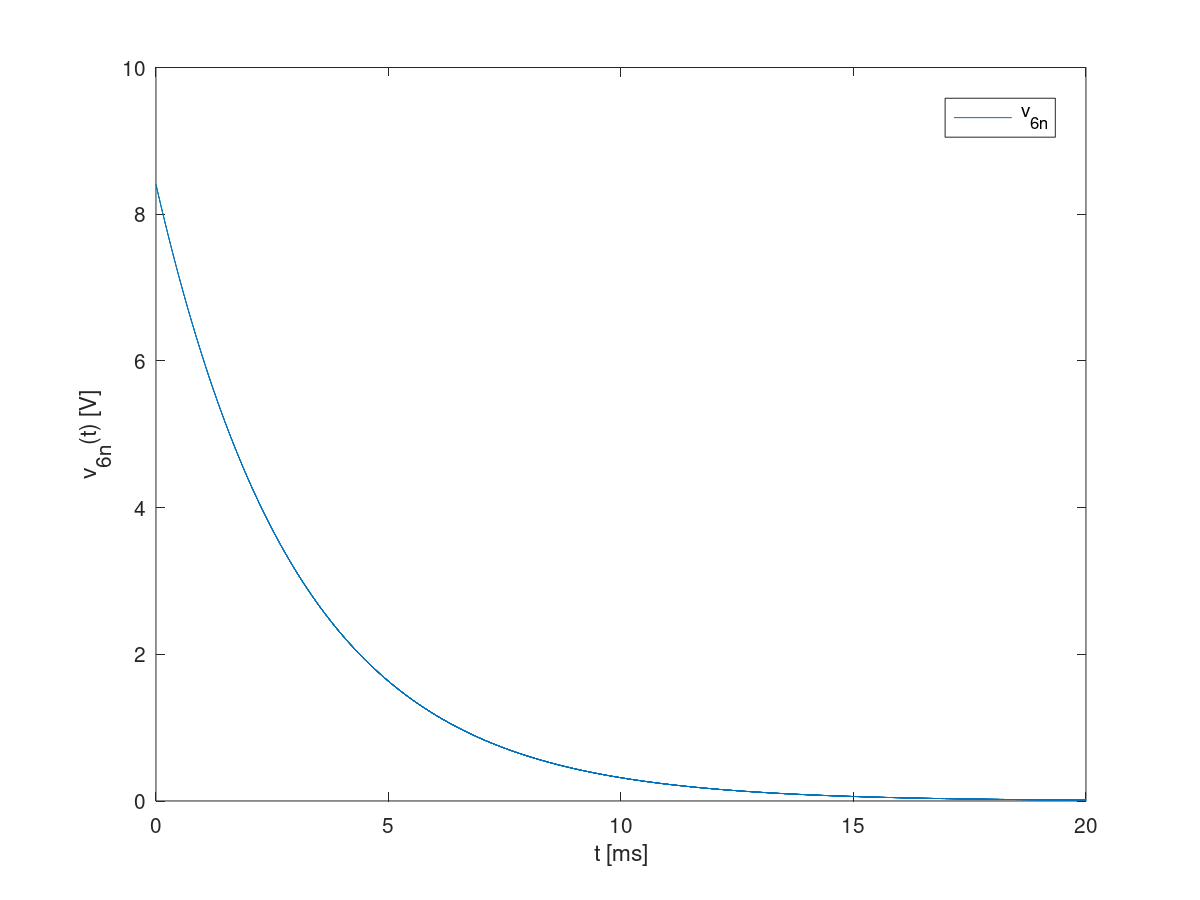
\includegraphics[width = 0.85\linewidth]{../mat/v6n.png}
        \caption{\textit{Plot of the natural solution for the voltage on node 6 in the interval $t\in[0,20]ms$ as shown on the plot}}
    \label{fig:natural}
\end{figure}
\subsection{Node analysis for $t\geq0$ - forced solution $v_6(t)$}

To complete the solution of the system, the forced solution needs to be determined. That was done using the nodal analysis method equivalent to \ref{eqnodos} but adding the current flowing thought the capacitor and changing the voltage source to it's new function ($V_s(t)=sin(2\pi f t)$ , $t\geq0$) resulting in the change of only this 3 equations.

\begin{equation}
    \begin{cases}
        V_1 - V_4 = -i e^{i 2\pi f C t} \hspace{15px} \text{(independent voltage source)}\\
        (V_5-V_2)G_3 + (V_5-V_4)G_4 + (V_5-V_6)G_5 + (V_8-V_7)G_7 + (V_8-V_6)i 2\pi f C = 0 \hspace{15px}\text{(supernodal equation)}\\
        (V_6-V_5)G_5 + (V_2-V_5)K_b + (V_6-V_8)i 2\pi f C = 0 \hspace{15px}\text{(node 6)}\\
    \end{cases}
\end{equation}

Note that the the complex phasors are being used instead of the normal sine function in order to obtain the complex amplitudes. Converting this system of equations to its matricial form, one can obtain:

\begin{equation}
\scalemath{0.8}{
    \begin{bmatrix}
     1 &  0      &  0 &    -1  &     0      &  0  &  0    &  0\\
     -G_1 & G_1+G_2+G_3 & -G_2  & 0   &  -G_3       &  0  &  0    &  0\\
     0   & -G_2-K_b    & G_2  & 0   &   K_b       &  0  &  0    &  0\\
     0   & 0        & 0   & 1 & 0       &  0  & 0   & 0\\
     0   & -G_3      &  0 &  -G_4  &   G_3+G_4+G_5 & -G_5-i 2\pi f C &  -G_7    & G_7+i 2\pi f C\\
     0   & K_b       & 0  &  0    & -G_5-K_b     & G_5+i 2\pi f C  & 0     &  -i 2\pi f C\\
     0   & 0        & 0  & -G_6   &  0         & 0   & G_6+G_7 & -G_7\\
     0   & 0        & 0  &  -K_dG_6    &  1         & 0   & K_dG_6     & -1
    \end{bmatrix} 
    \begin{bmatrix}
       V_1\\
        V_2\\
        V_3\\
        V_4\\
        V_5\\
        V_6\\
        V_7\\
        V_8
    \end{bmatrix}
    =
    \begin{bmatrix}
        -i e^{i 2\pi f C t}\\
        0\\
        0\\
        0\\
        0\\
        0\\
        0\\
        0
    \end{bmatrix}}
\label{eqnodos_forced}
\end{equation}

With the matrix defined, a program in octave was used to solve the system symbolically, to which was then substituted the frequency for $1000 Hz$ and, in order to obtain the complex amplitude, time for $0$, obtaining the values in Tab. \ref{tab:amplitude}.

The information that these complex amplitudes contain is the phase and amplitude of the oscillation, in this case forced, values that can be obtained through the complex amplitude norm and its argument, respectively, as it was done and the results are presented in Tab. \ref{tab:amplitude}.


\begin{table}[H]
    \begin{minipage}{.5\textwidth}
      \centering
      \begin{tabular}{c|c}
        \hline
     Node &  Complex Amplitude (v)\\ 
     \hline
    V(1) & -0.000000 + i(-1.000000)\\ V(2) & 0.000000 + i(-0.944378)\\ V(3) & -0.000000 + i(-0.827738)\\ V(5) & 0.000000 + i(-0.952375)\\ V(6) & -0.086752 + i(0.542623)\\ V(7) & 0.000000 + i(0.364103)\\ V(8) & 0.000000 + i(0.547147)\\ 
    \hline
      \end{tabular}
    \end{minipage}
    \begin{minipage}{.5\textwidth}
      \centering
      \begin{tabular}{c|c|c}
        \hline
          Node &  Amplitude (V) & Phase (rad)\\
          \hline
          V(1) & 1.000000 & -1.570796\\ 
V(2) & 0.944378 & -1.570796\\ 
V(3) & 0.827738 & -1.570796\\ 
V(5) & 0.952375 & -1.570796\\ 
V(6) & 0.549514 & 1.729330\\ 
V(7) & 0.364103 & 1.570796\\ 
V(8) & 0.547147 & 1.570796\\ 

          \hline
      \end{tabular}
    \end{minipage}
    \caption{Amplitudes for the forced solution osculations}
    \label{tab:amplitude}
\end{table}

With this information the forced solution can be plotted, in specific, in Fig.\ref{fig:forced}.

\begin{figure}[H]
    \centering
    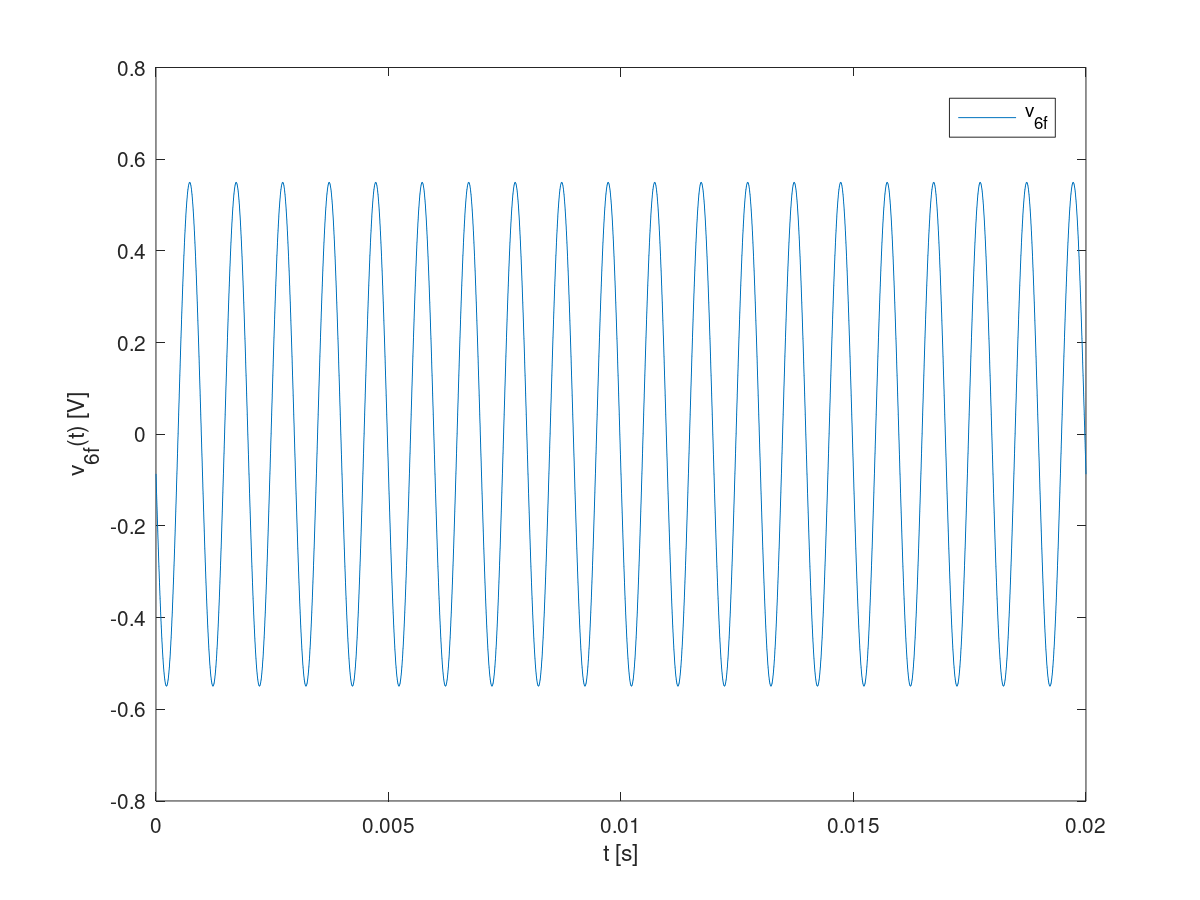
\includegraphics[width = 0.85\linewidth]{../mat/v6f.png}
        \caption{\textit{Plot of the forced solution for the voltage on node 6 in the interval $t\in[0,20]ms$ as shown on the plot}}
    \label{fig:forced}
\end{figure}

With both natural, obtained in Fig. \ref{fig:natural} and forced solutions, obtained in Fig. \ref{fig:forced} determined it's easy to add the 2 in order to obtain the complete solution, which for $V_6(t)$ is ploted in Fig. \ref{fig:complete}

\begin{figure}[H]
    \centering
    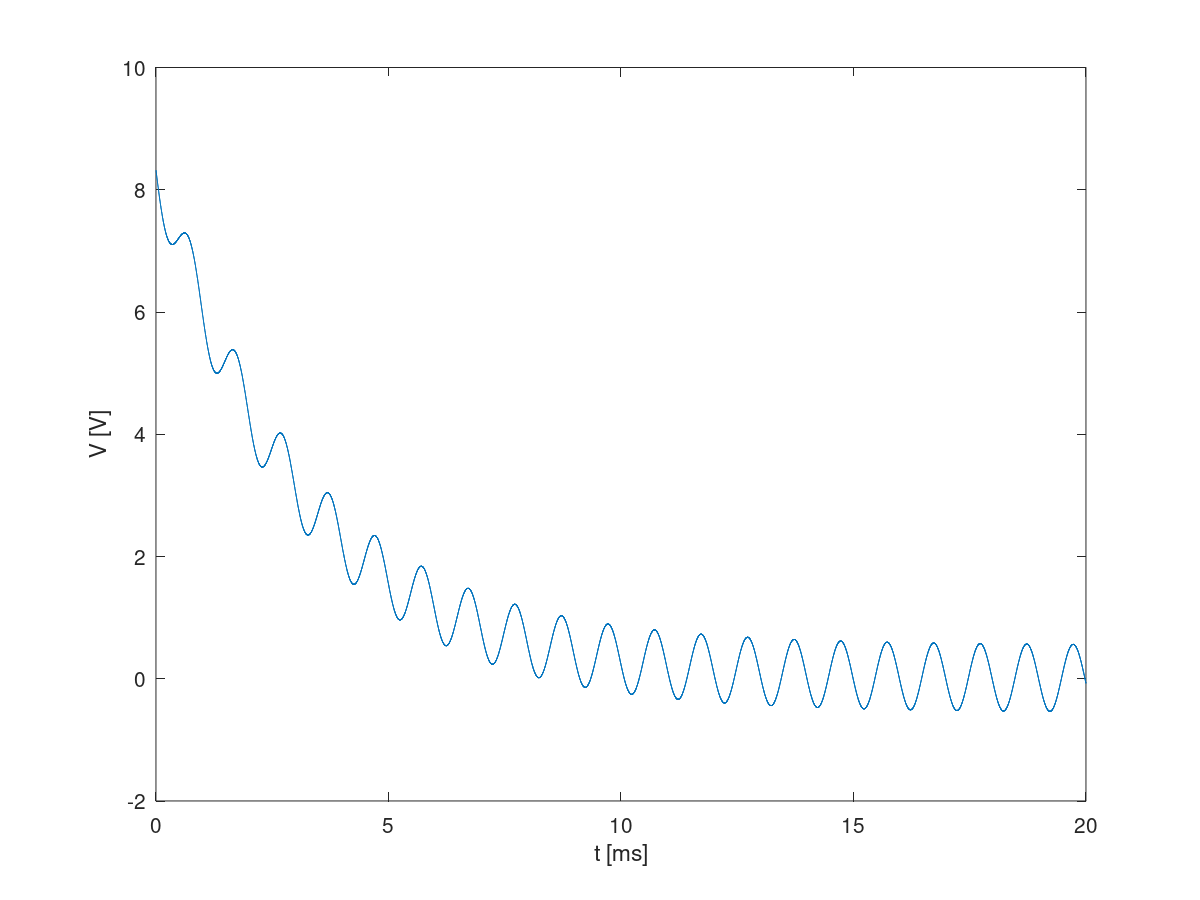
\includegraphics[width = 0.85\linewidth]{../mat/v6fn.png}
        \caption{\textit{Plot of the complete solution for the voltage on node 6 in the interval $t\in[0,20]ms$ as shown on the plot}}
    \label{fig:complete}
\end{figure}

For further understanding the behaving of the system, the voltage in node 6 and the input voltage can both be ploted for before and after $t=0$, by merging the results from the previous theoretical analysis, resulting in what is seen in Fig. \ref{fig:tudo}.

\begin{figure}[H]
    \centering
    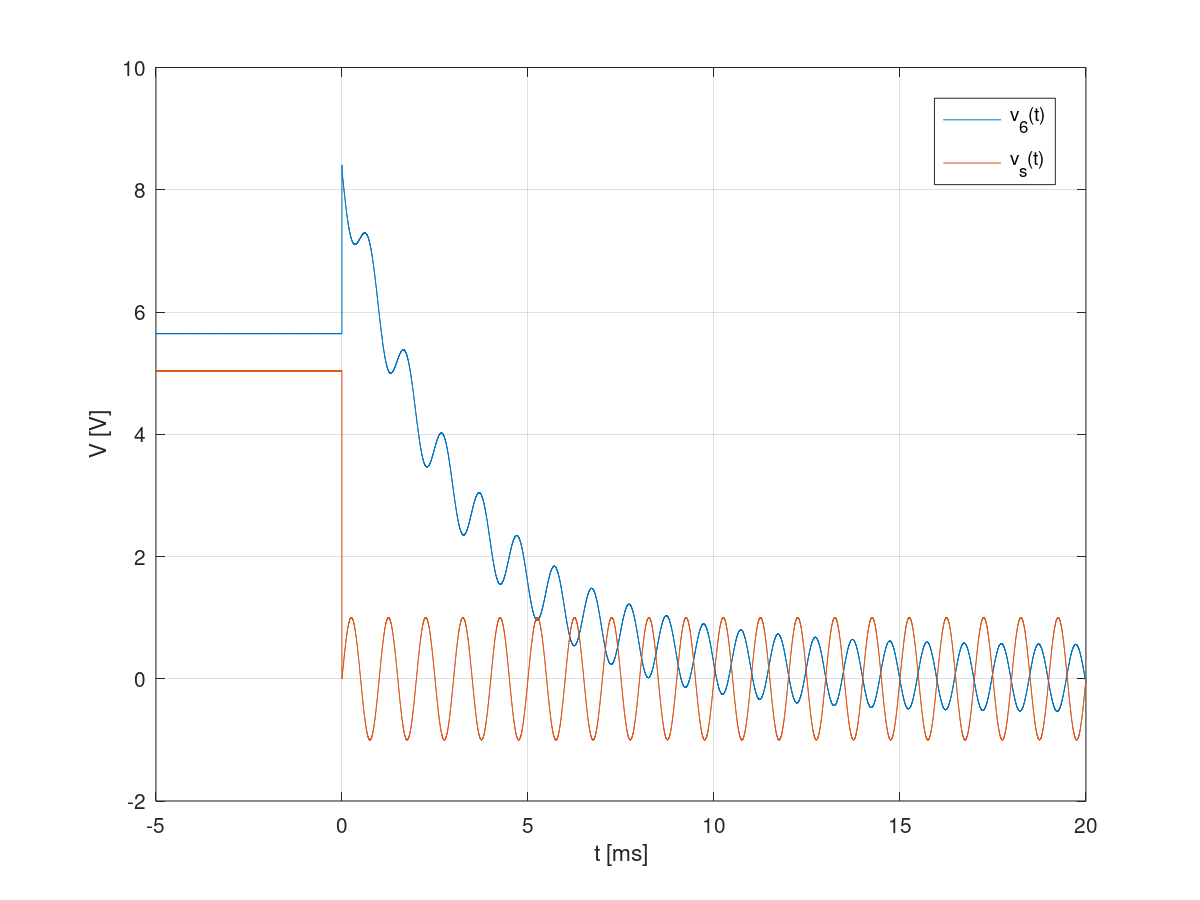
\includegraphics[width = 0.85\linewidth]{../mat/v6totsze.png}
        \caption{\textit{Plot of the complete solution for the voltage on node 6 and the input voltage  in the interval $t\in[-5,20]ms$ as shown on the plot}}
    \label{fig:tudo}
\end{figure}

As expected we can see that the discontinuity in the voltage source causes a discontinuity in the voltage in node 6, just not as intense and the system takes some time to reach the equilibrium and adapt to a behavior similar to its source. It's also notable that these 2 voltages are separated in phase by half a period.

\subsection{Magnitude and Phase as Functions of Frequency}

Once the system was solved symbolically, the complex amplitudes in function of the frequency could be obtain symbol by keeping $t=0$, and varying only the frequency, which in this case was done in the interval between $0.1$ and $10^6$ Hz. This time the goal was specifically to get the magnitude and the phase, instead of the complex amplitude, so as before were used the norm and the argument.

\begin{figure}[H]
    \centering
    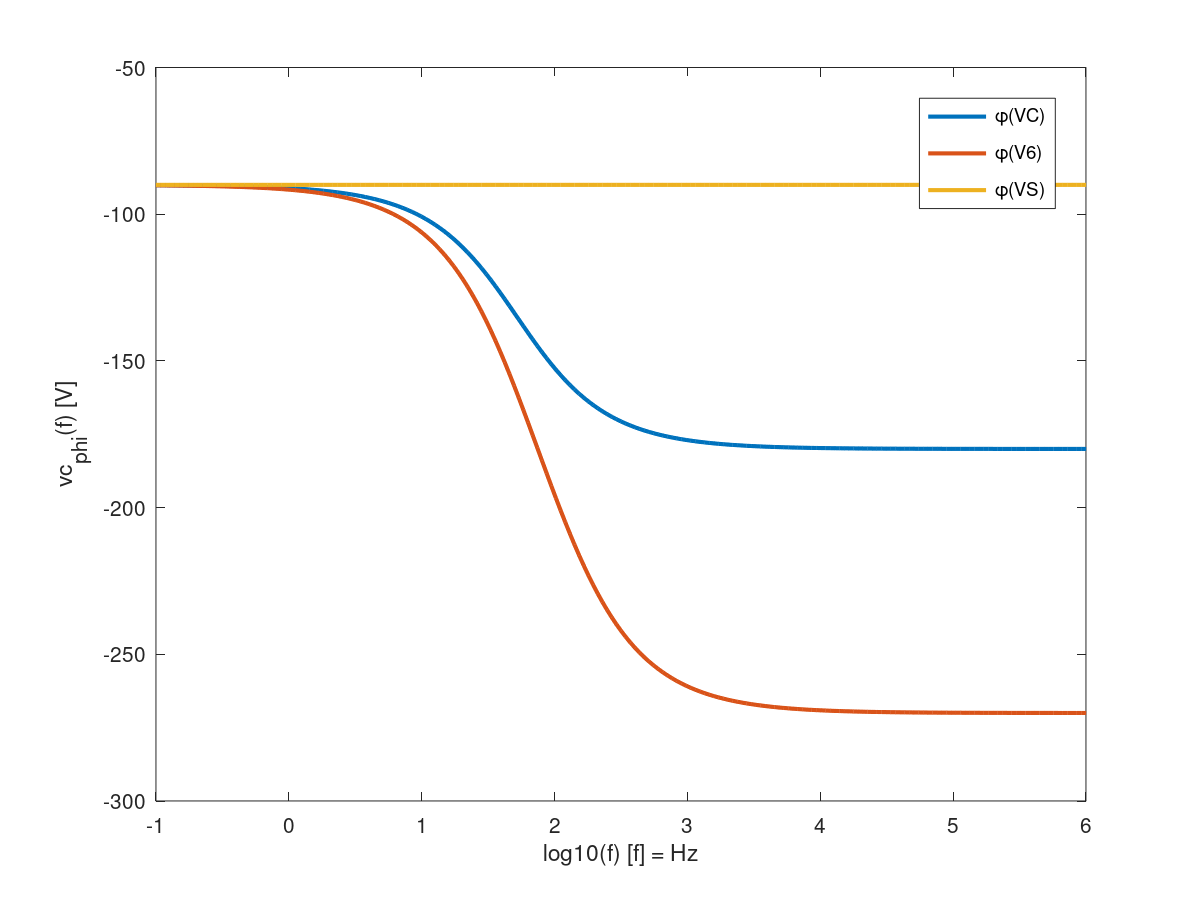
\includegraphics[width = 0.85\linewidth]{../mat/vcphi.png}
        \caption{\textit{Plot of the phase in function of the frequency. The frequency is presented in a logarithmic scale, contrary to the phase which is in linear scale in degrees.}}
    \label{fig:phase}
\end{figure}

As expected the phase for the voltage source is not dependent on the frequency, which was clear in the formula used to define it. More interestingly, the phase for both $V_c$ and $V_6$ seem to decrease around $50Hz$, stabilizing in a quarter and half a period, respectively, for higher frequencies.  


\begin{figure}[H]
    \centering
    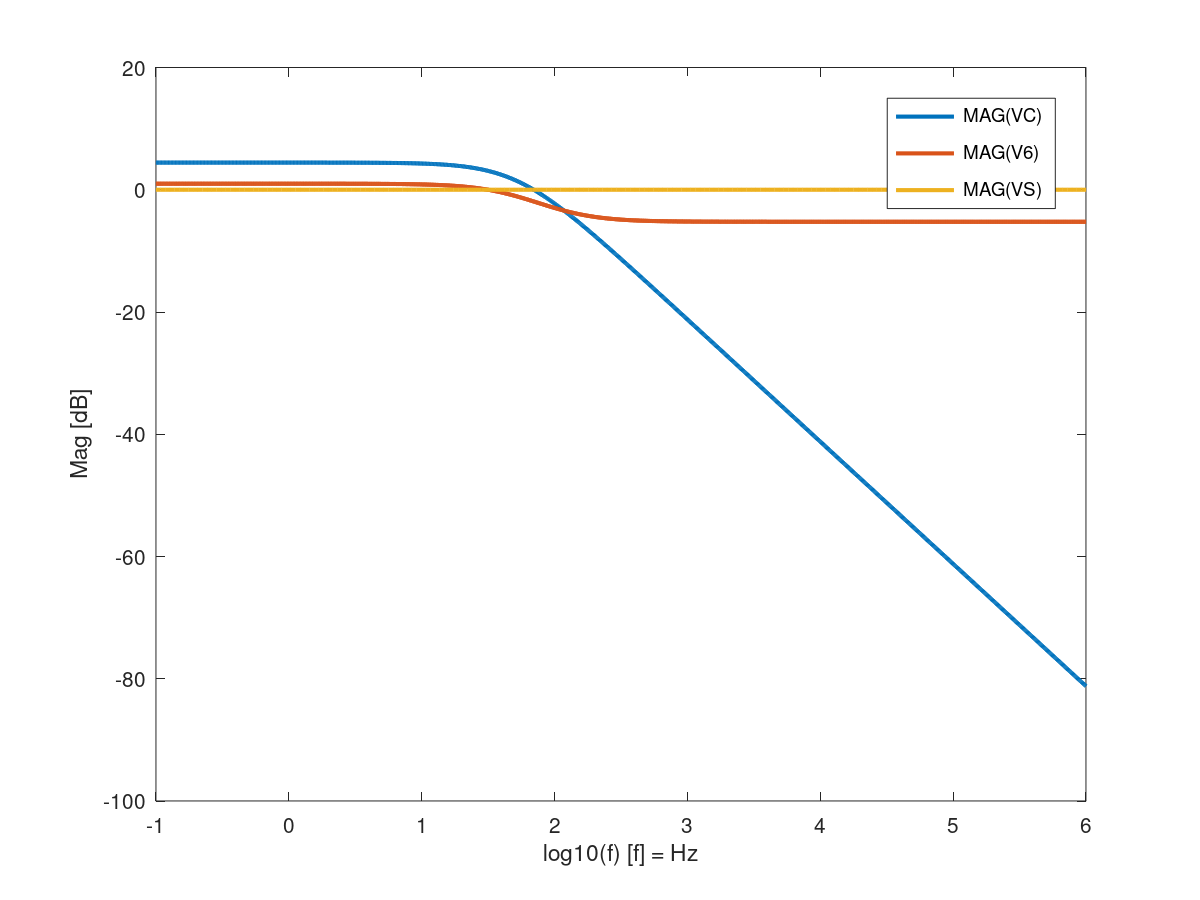
\includegraphics[width = 0.85\linewidth]{../mat/vcmag.png}
        \caption{\textit{Plot of the magnitude in function of the frequency. The frequency is presented in a logarithmic scale, as is the magnitude, which is in dB.}}
    \label{fig:magnitude}
\end{figure}

With amplitude $1$, $V_s$ has a constant magnitude for any frequency as expected, contrary to the other amplitudes that decrease with the increase in frequency, and for really high oscillation in the source, the amplitude of the oscillation in node 6 is practically 0. The critical frequency seems to be at $80Hz$.
\section{Simulation Analysis}

To be sure of the values obtained in \ref{sec:theo}, we made use of Ngspice, a more stable version of the Berkeley SPICE, which is an "open source spice simulator for electric and electronic circuits", as stated in \cite{ngsite}. The code used was the following, \\

{\itshape
TCFELab1 \par
.options savecurrents \\\par

Vin 1 4 5.03847501972 \par
Id 0 6 1.01674167773m \par

$V_{dumb}$ CFP1 7 0 \\\par

R1 2 1 1.03994439216k \par
R2 3 2 2.07923431764k \par
R3 2 5 3.06168544529k \par
R4 4 5 4.09516986362k \par
R5 5 6 3.00136467001k \par
R6 4 CFP1 2.03324628446k \par
R7 7 0 1.02216788331k \\\par

Gb 6 3 2 5 7.01505323139m \par
Hc 5 0 $V_{dumb}$ 8.37372457746k \\\par

.op\par
.control\par
    run\par
    print all\par
.endc\par
.end
}

\vspace{10px}
The first line of this code is the title of the simulation itself, which is followed by the option to save currents, a command that allows the program to, when printing all the variables, also print the currents flowing in every component of the circuit. Then, \textit{Vin} and \textit{Id} are the $V_a$, $I_d$ corresponding to what is shown in Fig. \ref{fig:nodal_scheme}. $V_{dumb}$ is a dumb voltage source that was introduced for a specific reason that will be later explained. In this simulation, we chose node 8 to be GND, which, by Ngspice standards, has to be named node 0.\\

After this, all the resistances were declared in the form \textit{R<name> <n+> <n-> <value>}, where n+ and n- mean the positive and negative nodes of the electronic component, according to the schematics shown in Fig.\ref{fig:polos}. \\

\begin{figure}[h]
    \centering
    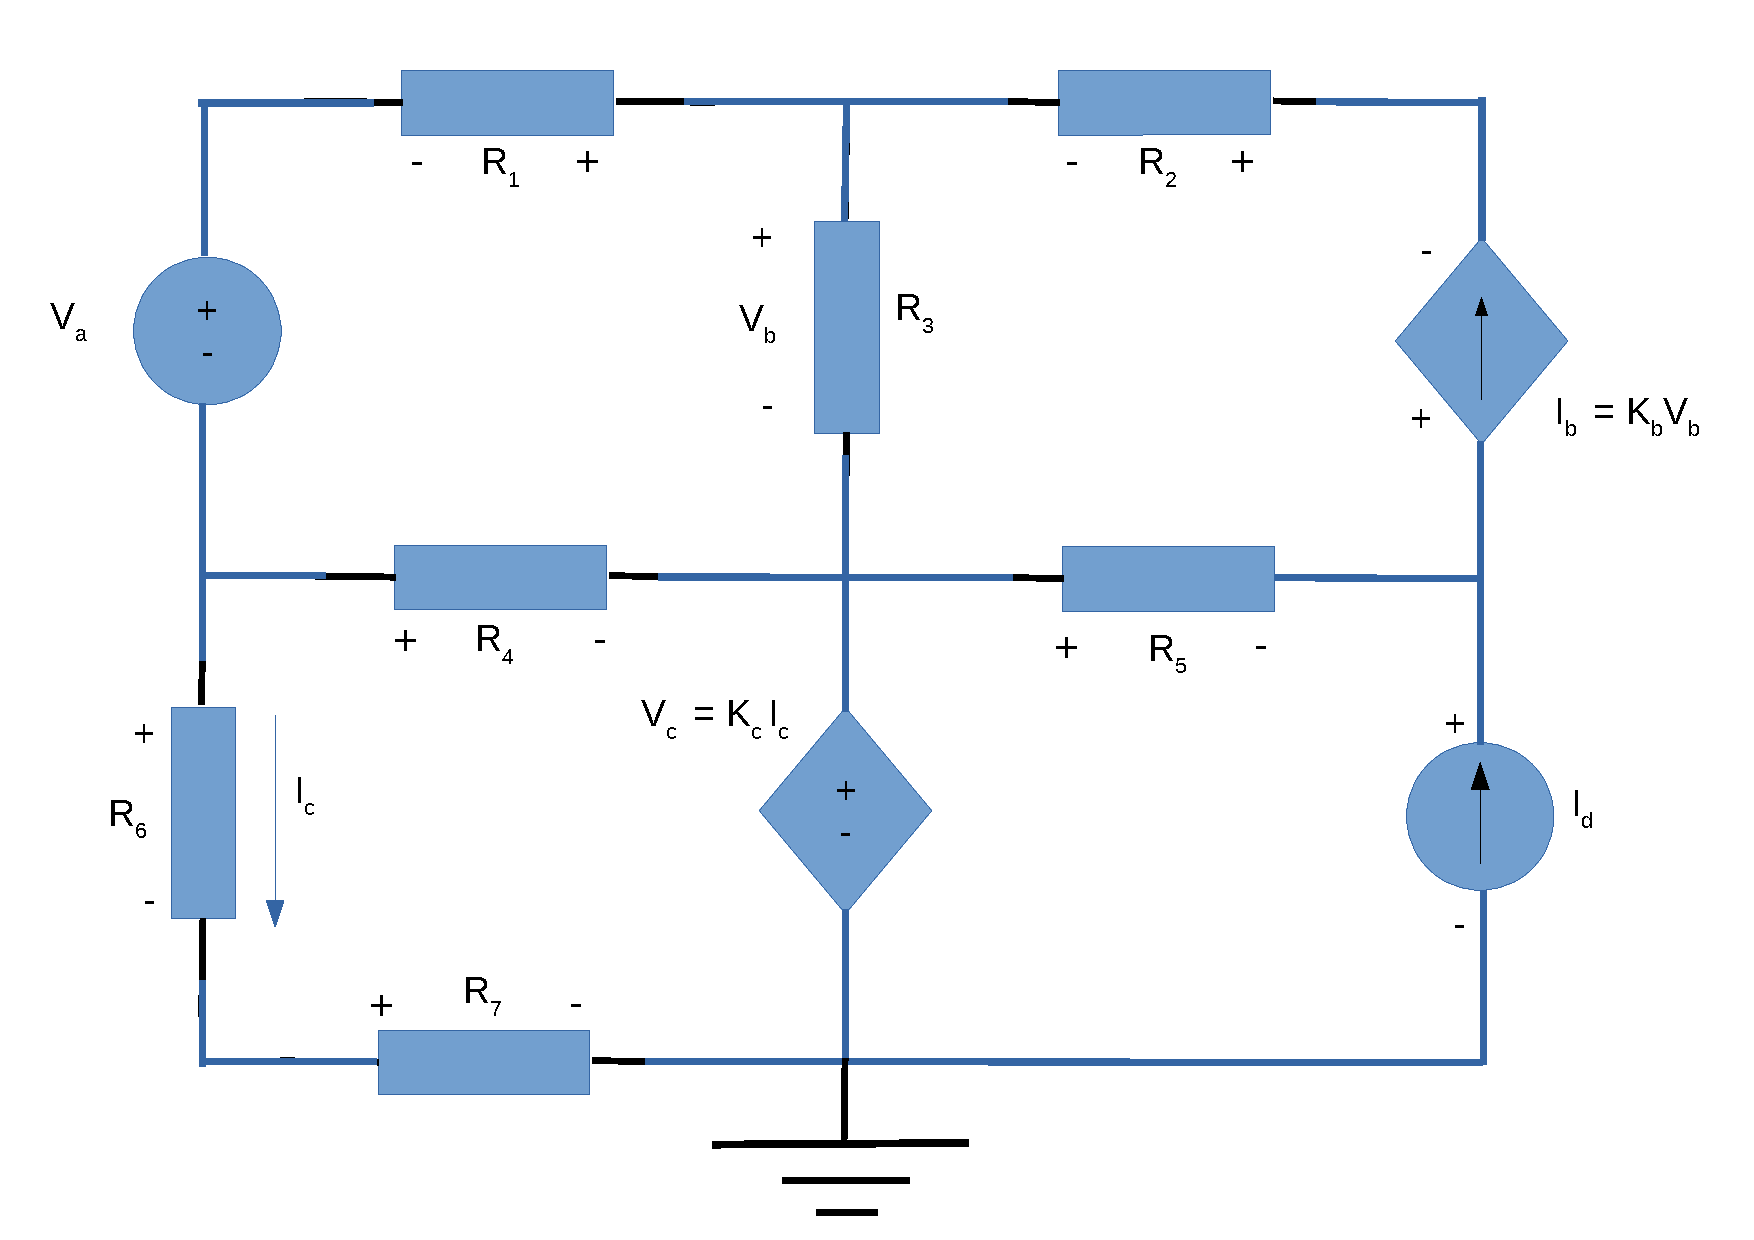
\includegraphics[width = 0.7\linewidth]{esquemacpolos.pdf}
        \caption{\textit{Representation of the convention used to the Ngspice simulation. In the figure above, one can see the conventioned positive and negative terminal for each branch}}
    \label{fig:polos}
\end{figure}

Afterwards, $Gb$ and $Hc$ stand for the voltage-controlled current source $I_b$ and current-controlled voltage source $V_c$ respectively. The first two parameters received by $Gb$ are its positive and negative nodes as expected and then the two nodes where it should calculate the corresponding potential. For $Hc$, the third parameter is $V_{dumb}$ which, as promised, is a voltage source that was introduced for the single purpose that current-controlled voltage sources in \textit{Ngspice} take as a third parameter only voltage sources through which the current in question is flowing through. Thus, because the purpose is to retrieve $I_c$, a dumb voltage source was added after $R_6$, creating a new node that was called CFTP1, which is where $R_6$ then connects. To not alter the circuit at all, the actual induced voltage by $V_{dumb}$ is 0V, thus CFTP1 and node 7 are in short circuit, i.e., the circuit does not "see" $V_{dumb}$. At last, inside \textit{control}, the simulation is ran and everything is printed out, giving the following output:\\\par


\begin{table}[H]
\setlength{\tabcolsep}{10pt}
\renewcommand{\arraystretch}{1.1}
\centering
    \begin{tabular}{||c|c||}
    \hline
    Name & Current/Voltage [A/V]\\
    \hline
    @cb[i] & 0.000000e+00\\ \hline
@ce[i] & 0.000000e+00\\ \hline
@q1[ib] & 7.022567e-05\\ \hline
@q1[ic] & 1.404513e-02\\ \hline
@q1[ie] & -1.41154e-02\\ \hline
@q1[is] & 5.765392e-12\\ \hline
@rc[i] & 1.411536e-02\\ \hline
@re[i] & 1.411536e-02\\ \hline
@rf[i] & 7.022567e-05\\ \hline
@rs[i] & 0.000000e+00\\ \hline
v(1) & 0.000000e+00\\ \hline
v(2) & 0.000000e+00\\ \hline
base & 2.254108e+00\\ \hline
coll & 5.765392e+00\\ \hline
emit & 1.411536e+00\\ \hline
vcc & 1.000000e+01\\ \hline

    \end{tabular}
\vspace{0.2 cm}
\caption{Values for several variables declared in the .net file.}
\label{max}
\end{table}


\vspace{10px}

The values obtained were expected in some way given the results obtained in the theoretical analysis and that were presented in the last section. The reader can check the results knowing that $V_b = V_2 -V_5$ and $V_c = V_5$.\\

However, due to \textit{machine epsilons} and related things, some decimal places might be a bit different. The main cause of this is that Ngspice also uses, whenever possible, nodal analysis. Thus, for solving matrix \ref{eqnodos}, one has to be aware that inverting a 9x9 or 7x7 matrix will introduce a significant margin of error, which explains a possible observable difference in the results obtained, specially between this simulation and the mesh analysis.

\section{Side by side comparison between analysis results}
\label{sec:sidebyside}

\begin{table}[H]
    \begin{minipage}{.4\textwidth}
    \begin{table}[H]
    \centering
    \small
    \begin{tabular}{|c|c|c|c|}
          \hline
          Node/Branch & $@(i) [A]/ v [V]$\\
          \hline
          @cb[i] & 0.000000e+00\\ \hline
@ce[i] & 0.000000e+00\\ \hline
@q1[ib] & 7.022567e-05\\ \hline
@q1[ic] & 1.404513e-02\\ \hline
@q1[ie] & -1.41154e-02\\ \hline
@q1[is] & 5.765392e-12\\ \hline
@rc[i] & 1.411536e-02\\ \hline
@re[i] & 1.411536e-02\\ \hline
@rf[i] & 7.022567e-05\\ \hline
@rs[i] & 0.000000e+00\\ \hline
v(1) & 0.000000e+00\\ \hline
v(2) & 0.000000e+00\\ \hline
base & 2.254108e+00\\ \hline
coll & 5.765392e+00\\ \hline
emit & 1.411536e+00\\ \hline
vcc & 1.000000e+01\\ \hline

          \hline
    \end{tabular}
    \caption{Solution from simulation.}
    \label{tab:ngs_tau}
    \end{table}
    \end{minipage}
    \begin{minipage}{.29\textwidth}
      \centering
      \begin{tabular}{c|c}
        \hline
          Branch &  Current (A) \\
          \hline
          \input{"currents_branches_first_alienea.tex"}
          \hline
      \end{tabular}
    \label{tab:current2}
    \caption{Currents from theoretical solution}
    \end{minipage}
    \begin{minipage}{.29\textwidth}
      \begin{equation} \Vec{b} = \begin{bmatrix}  5.0385\\  4.7582\\  4.1705\\      -0\\  4.7985\\  5.6468\\ -1.8345\\ -2.7568 \end{bmatrix} \label{eqsol} \end{equation}
      \caption{Voltages from theoretical solution}
      \end{minipage}
    \caption{Solution for voltages for all nodes and current for all branches for $t<0$.}
    \end{table}

The only difference found between the 2 solutions, for the digits presetned here are for $V_3$ and $V_6$, but only in the last digit presented, meaning a difference around $10^{-6} V$. Differences that are probably result of numerical errors, rather than real differences in solutions.

\begin{figure}[H]
\hspace{-10mm}
  \subfigure[Theoretical analysis]{% 
    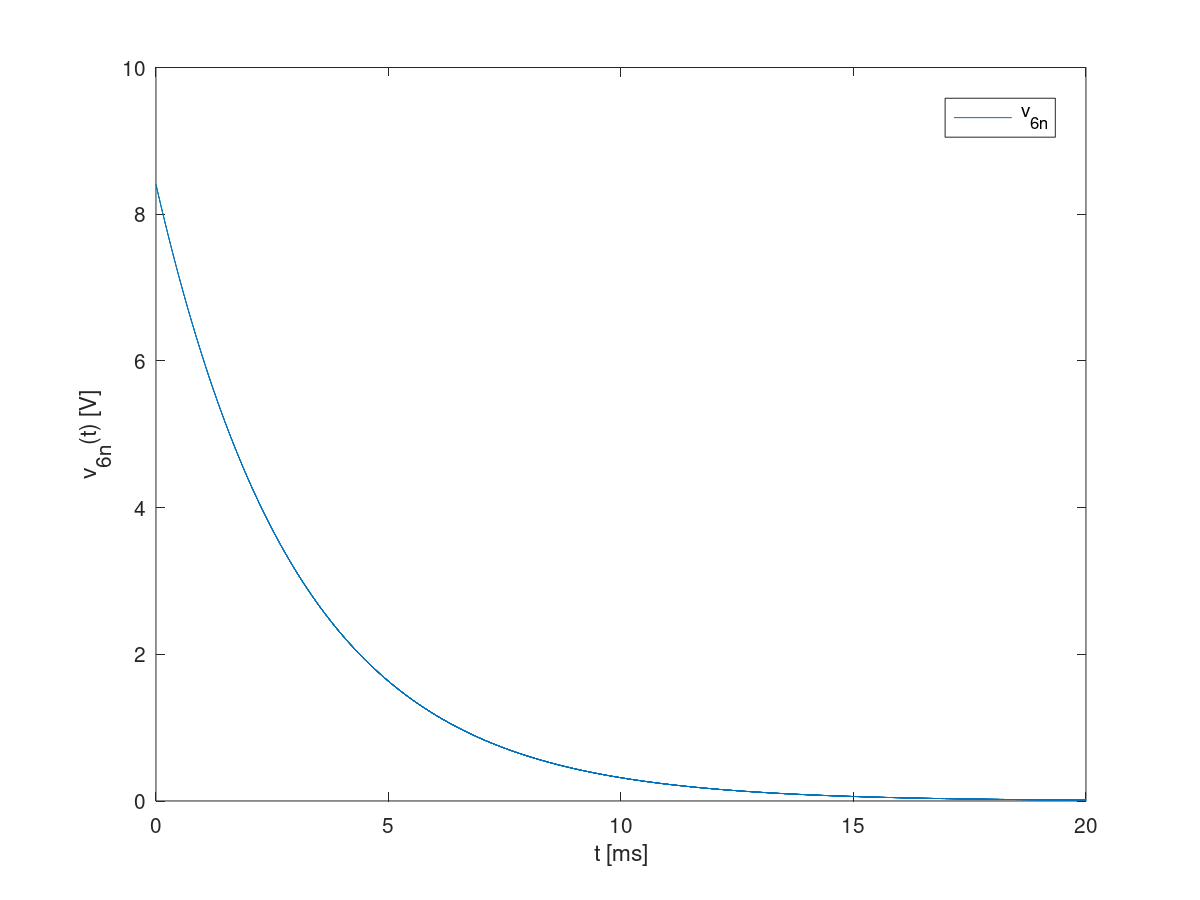
\includegraphics[width=.6\textwidth]{../mat/v6n.png} \label{fig:teo_nat} 
  } 
  \subfigure[Simulation analysis]{% 
    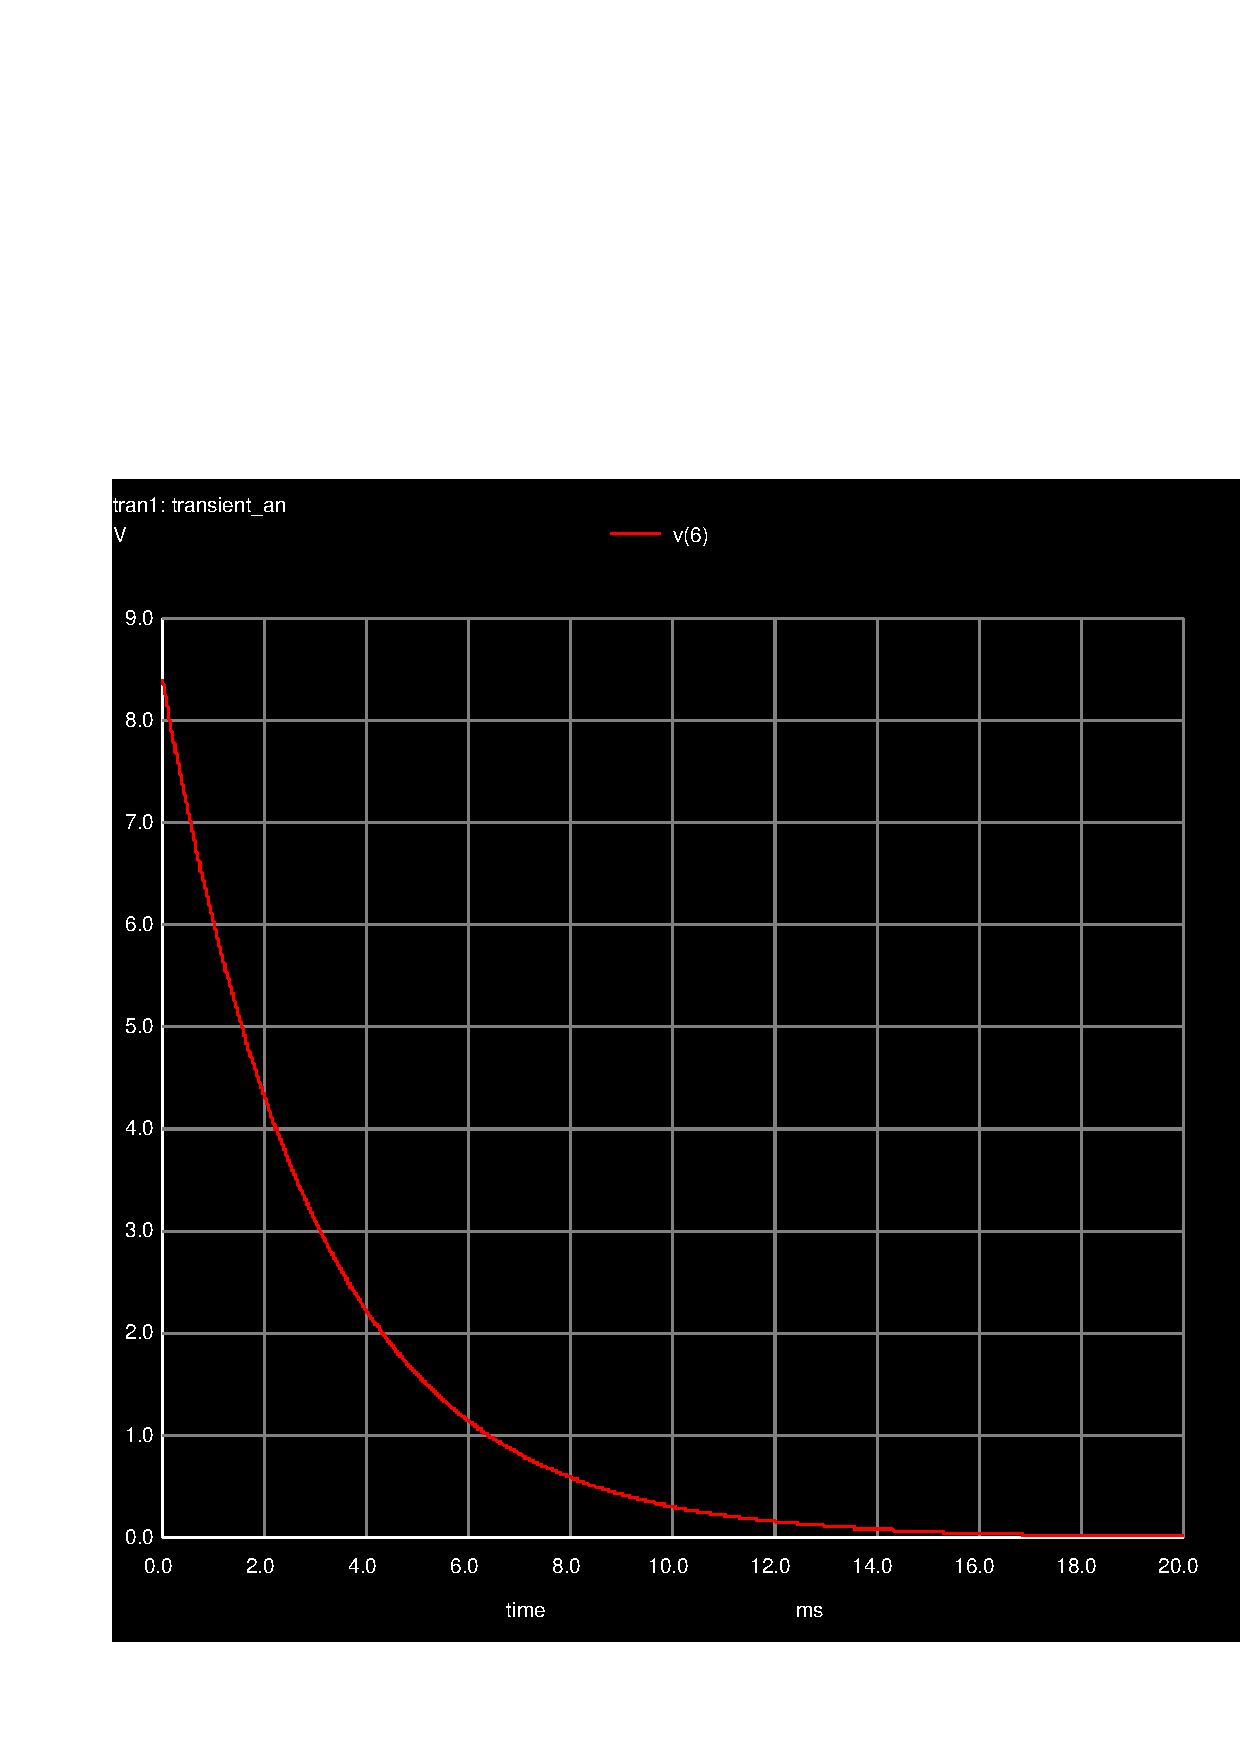
\includegraphics[width=.45\textwidth]{../sim/trans3.pdf} \label{fig:sim_nat} 
  } 
  \caption{Natural solution for voltage in node 6 for $t=[0,20]$.} 
\end{figure}

The solution for the natural solution in node 6 appears to be exactly the same.

\begin{figure}[H]
\hspace{-10mm}
  \subfigure[Theoretical analysis]{% 
    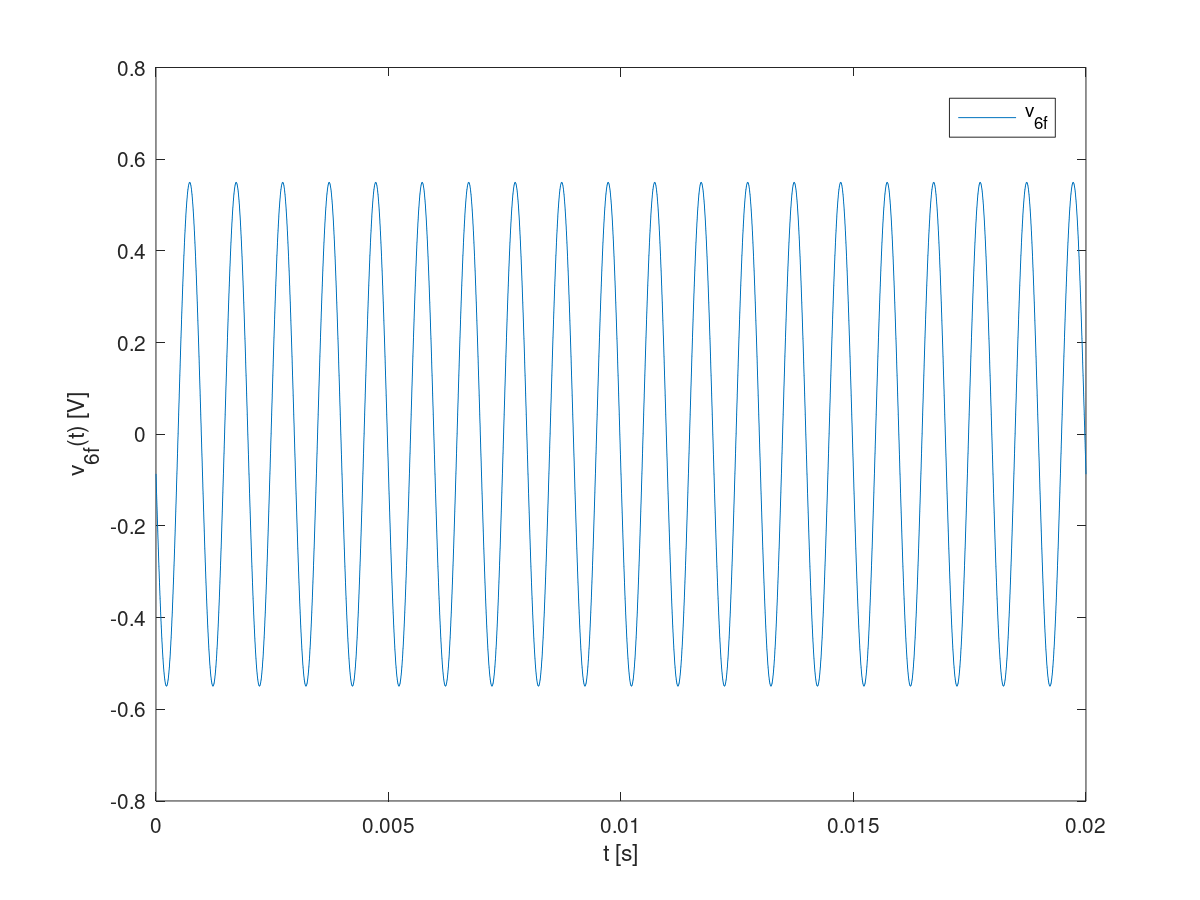
\includegraphics[width=.6\textwidth]{../mat/v6f.png} \label{fig:teo_for} 
  } 
  \subfigure[Simulation analysis]{% 
    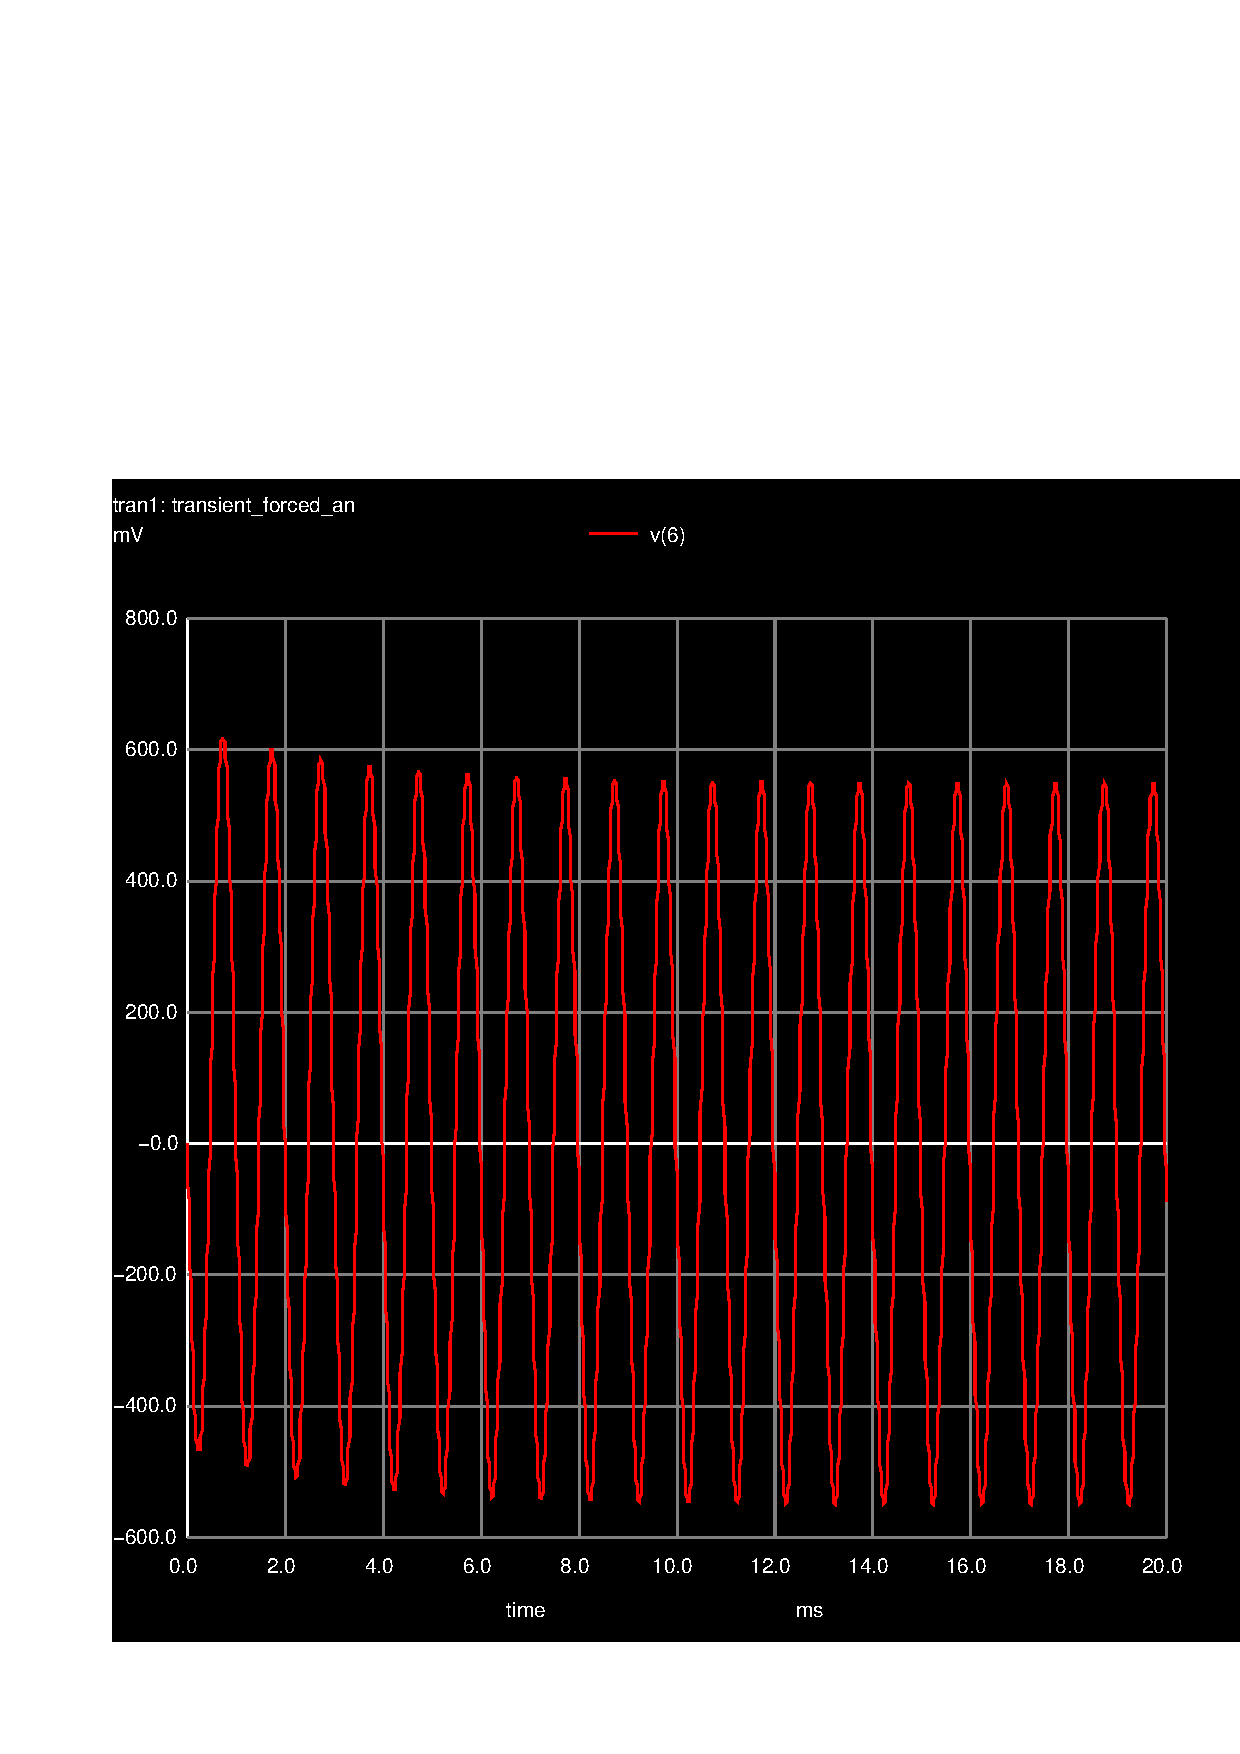
\includegraphics[width=.45\textwidth]{../sim/trans4.pdf} \label{fig:sim_for} 
  } 
  \caption{Forced solution for voltage in node 6 for $t=[0,20]$.} 
\end{figure}

As mentioned before, the only difference found between these 2 solution is that in the forced solution a small offset seems to exist in the first moments of the oscillation, but appears to stabilize on the expected solution.

\begin{figure}[H]
\hspace{-10mm}
  \subfigure[Theoretical analysis]{% 
    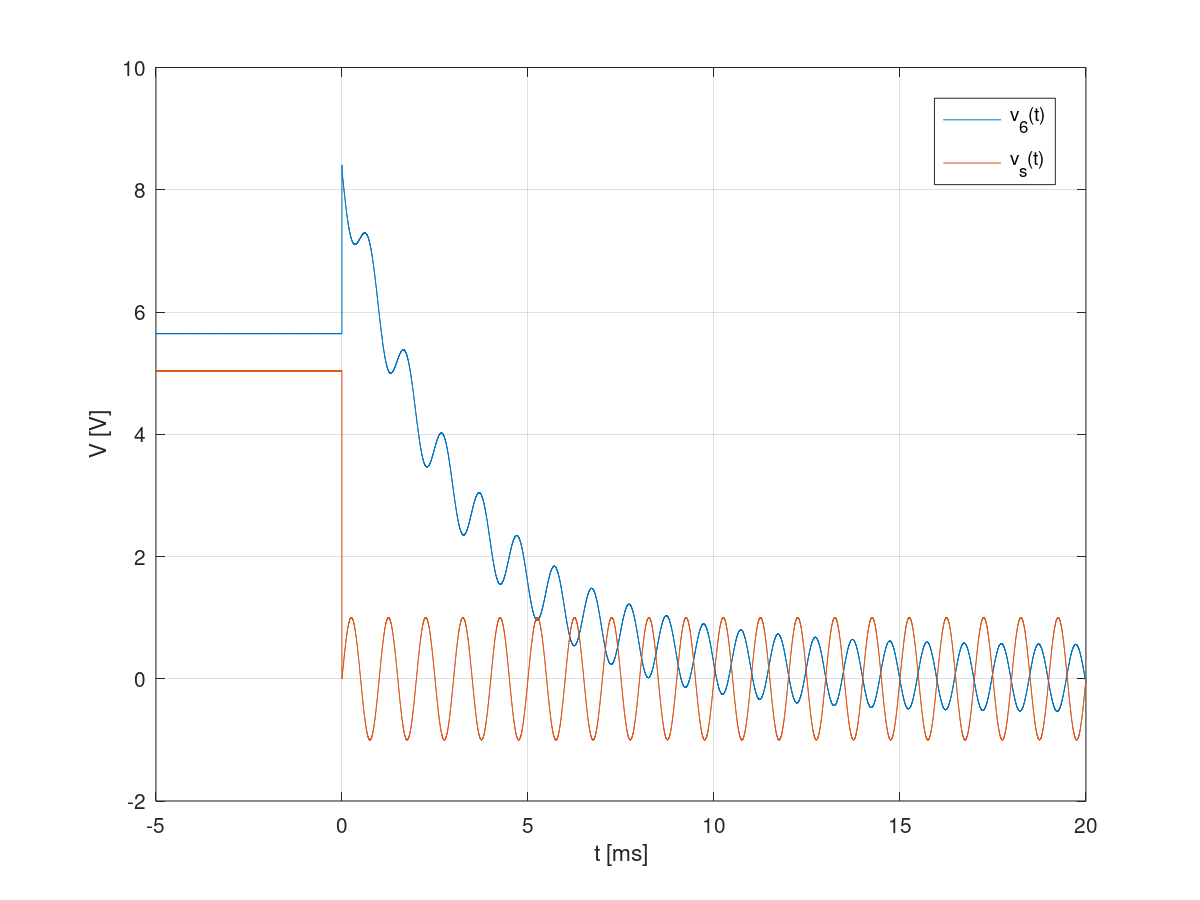
\includegraphics[width=.6\textwidth]{../mat/v6totsze.png} \label{fig:teo_comp} 
  } 
  \subfigure[Simulation analysis]{% 
    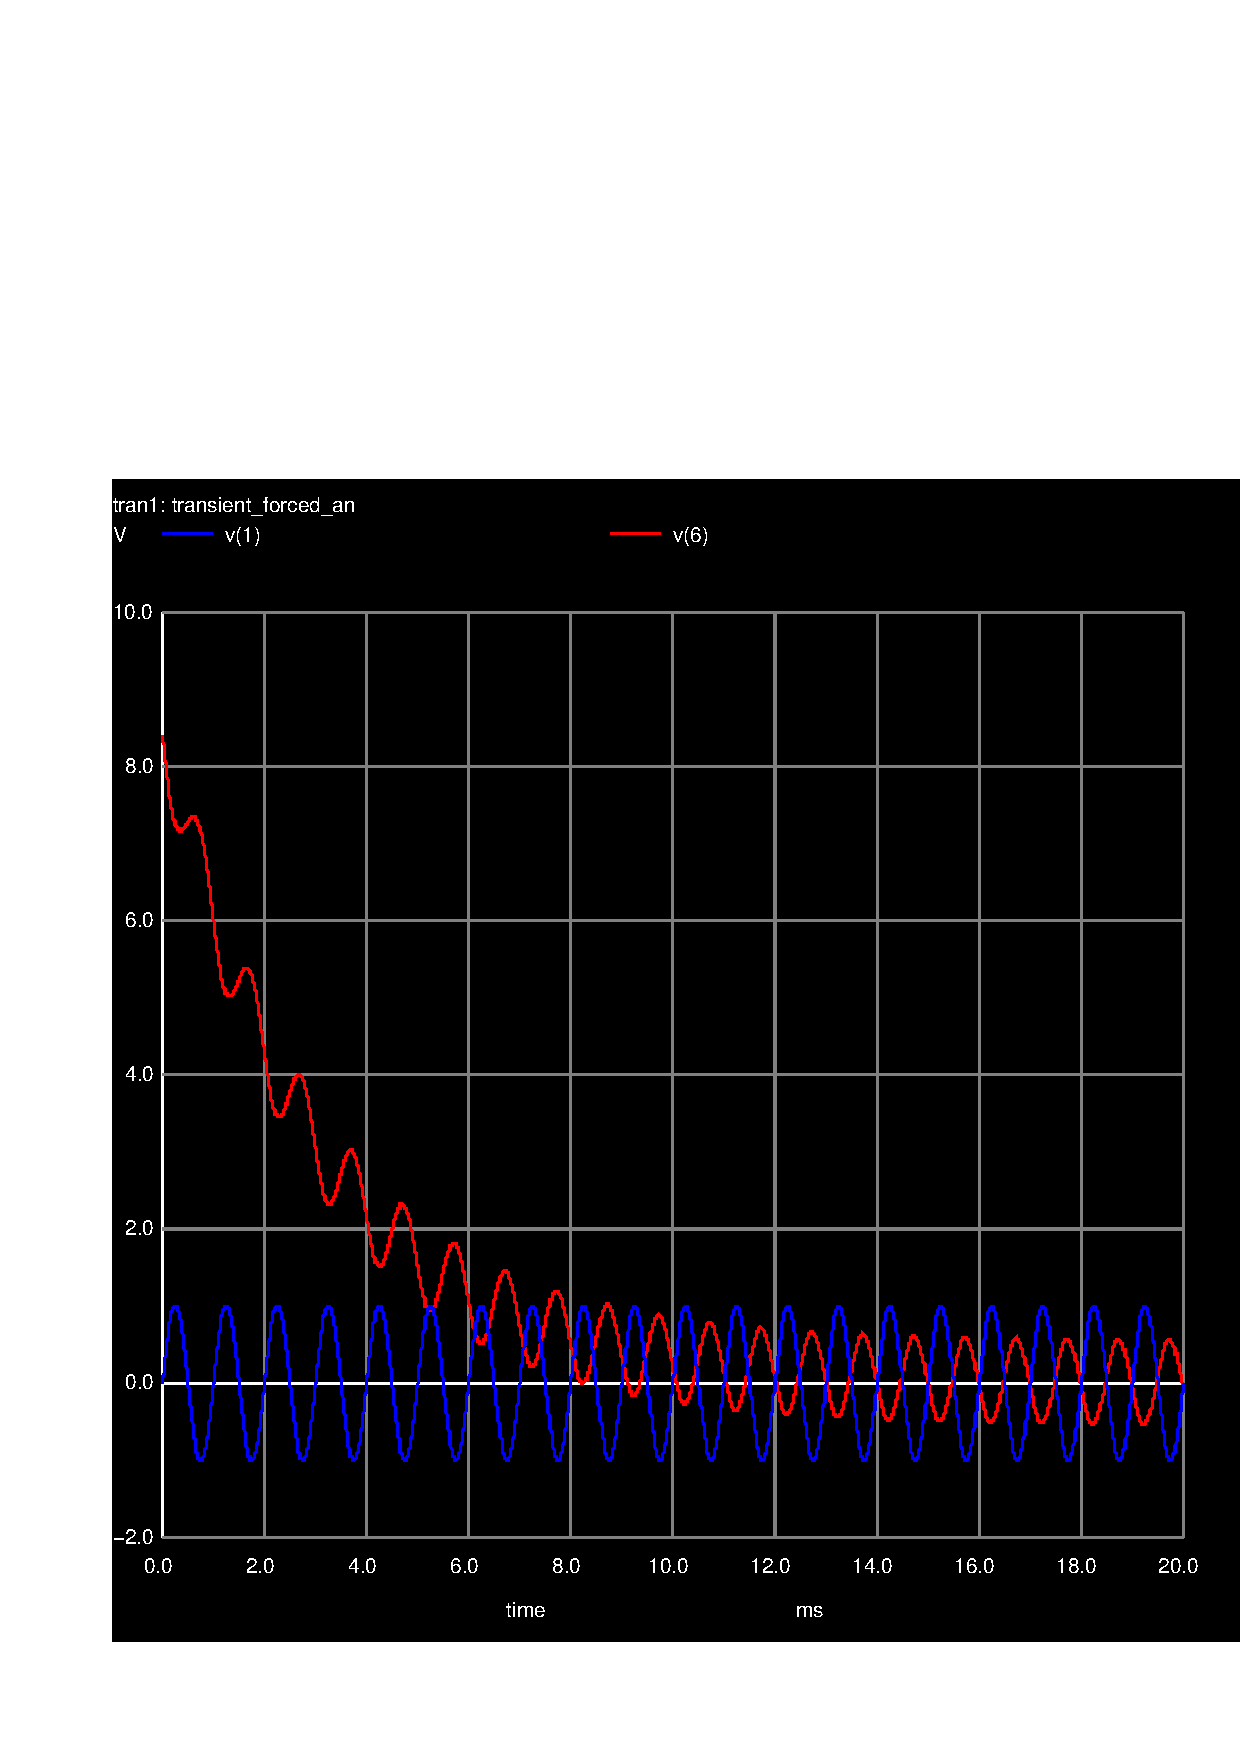
\includegraphics[width=.45\textwidth]{../sim/trans5.pdf} \label{fig:sim_comp} 
  } 
  \caption{Complete solution for voltage in node 6 for $t=[-5,20]$ and $t=[0,20]$.} 
\end{figure}

Besides the part of the forced solution that is now impossible to notice, the plots looks identical even in close inspection.

\begin{figure}[H]
\hspace{-10mm}
  \subfigure[Theoretical analysis]{% 
    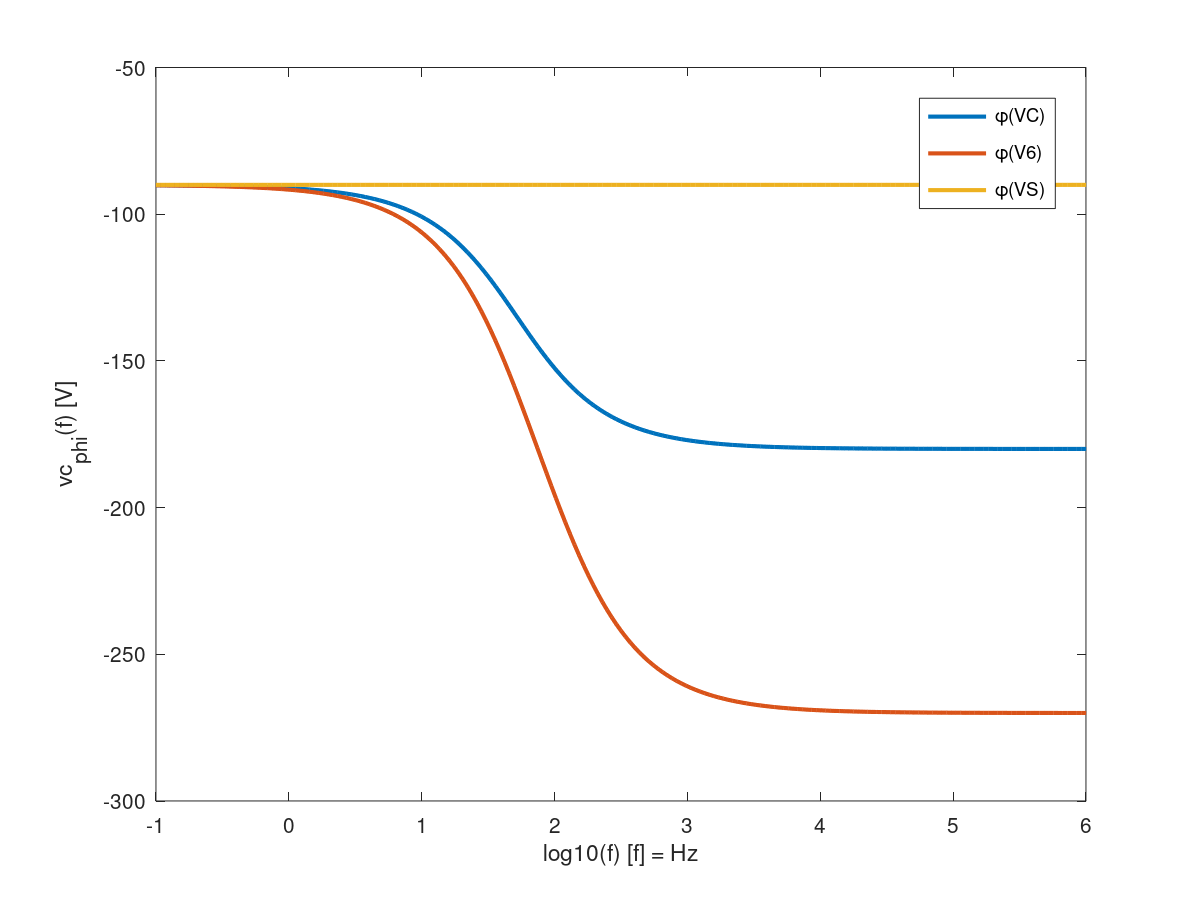
\includegraphics[width=.6\textwidth]{../mat/vcphi.png} \label{fig:teo_phi} 
  } 
  \subfigure[Simulation analysis]{% 
    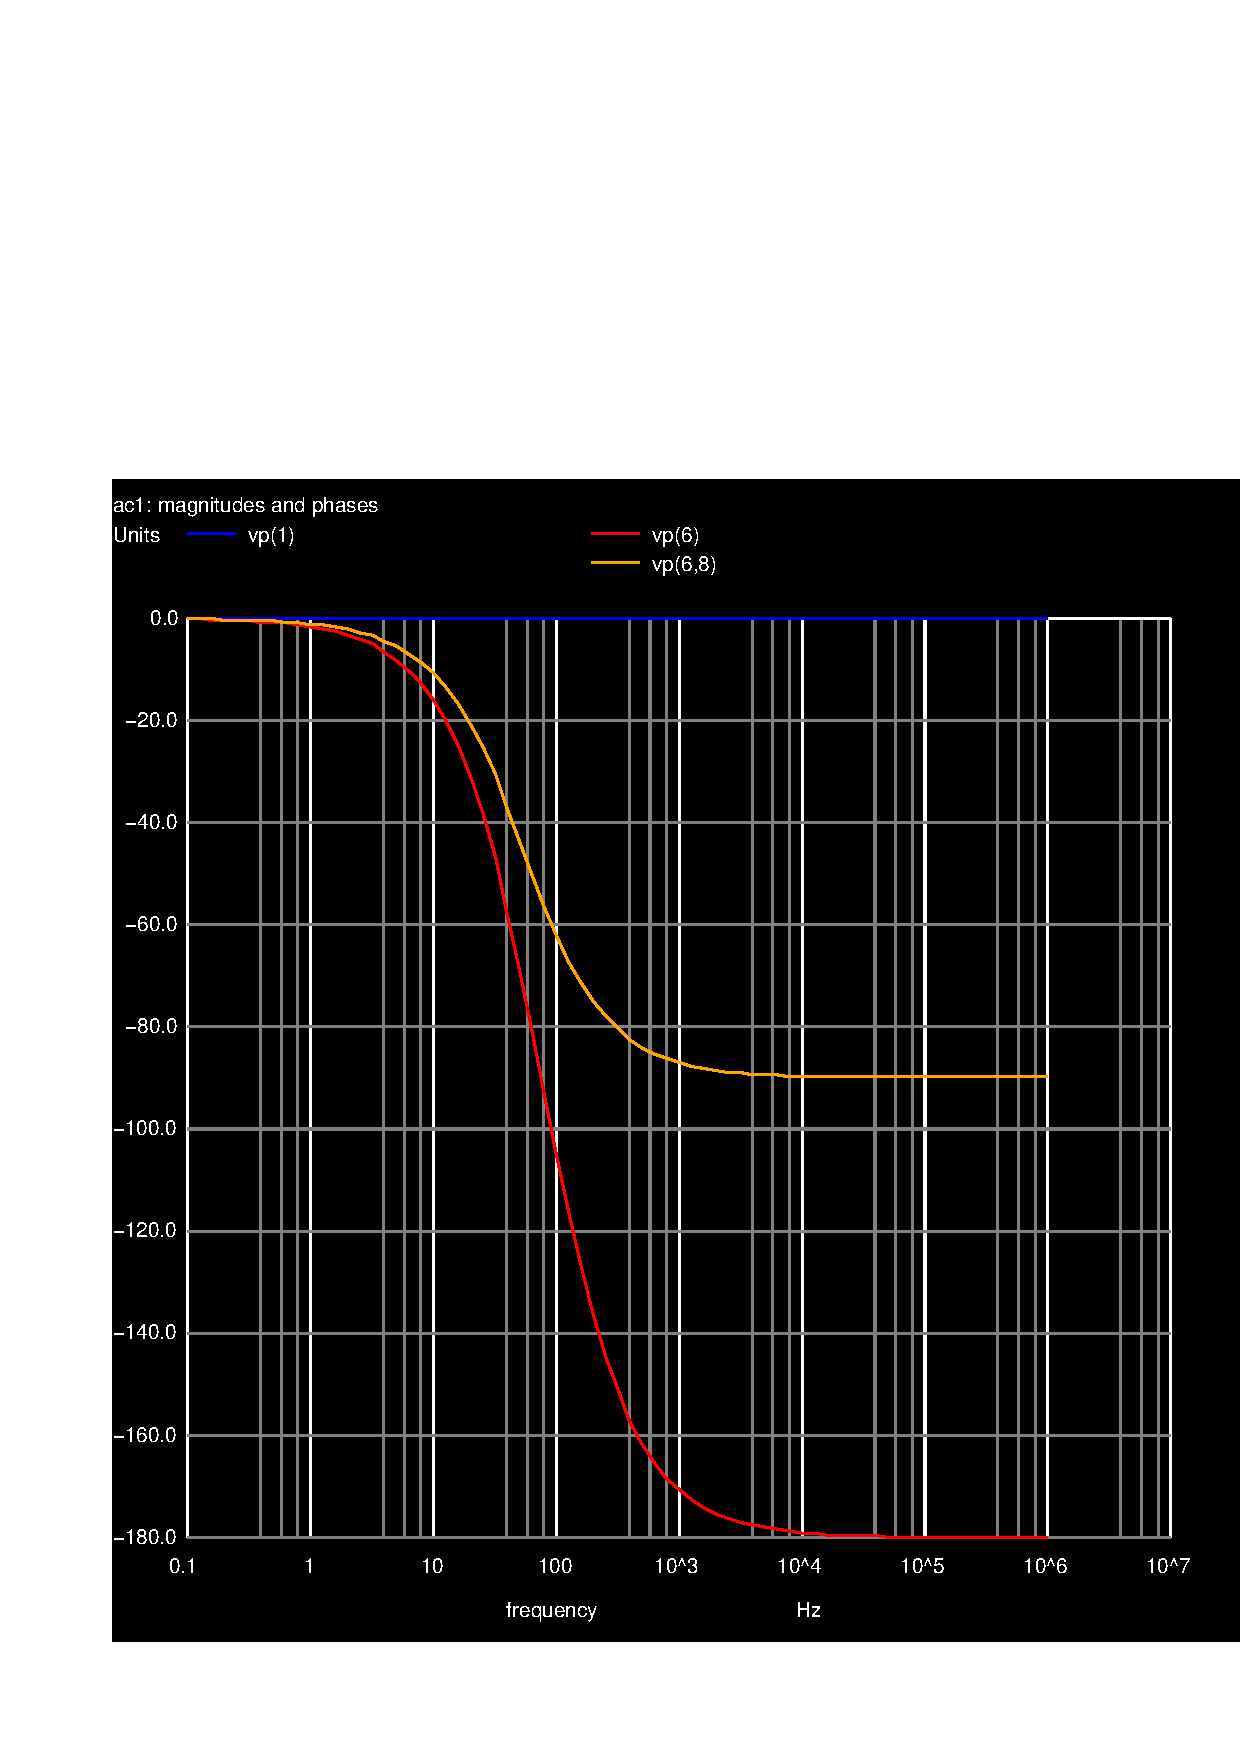
\includegraphics[width=.45\textwidth]{../sim/zezoca.pdf} \label{fig:sim_phi} 
  } 
  \caption{Phase difference as a function of the frequency of the voltage source.} 
\end{figure}

As mentioned before the same transition to a phase difference of a quarter and half a period is seen but \textit{Ngspice} automatically offsets the phases in order for the source to be at 0 degrees.


\begin{figure}[H]
\hspace{-10mm}
  \subfigure[Theoretical analysis]{% 
    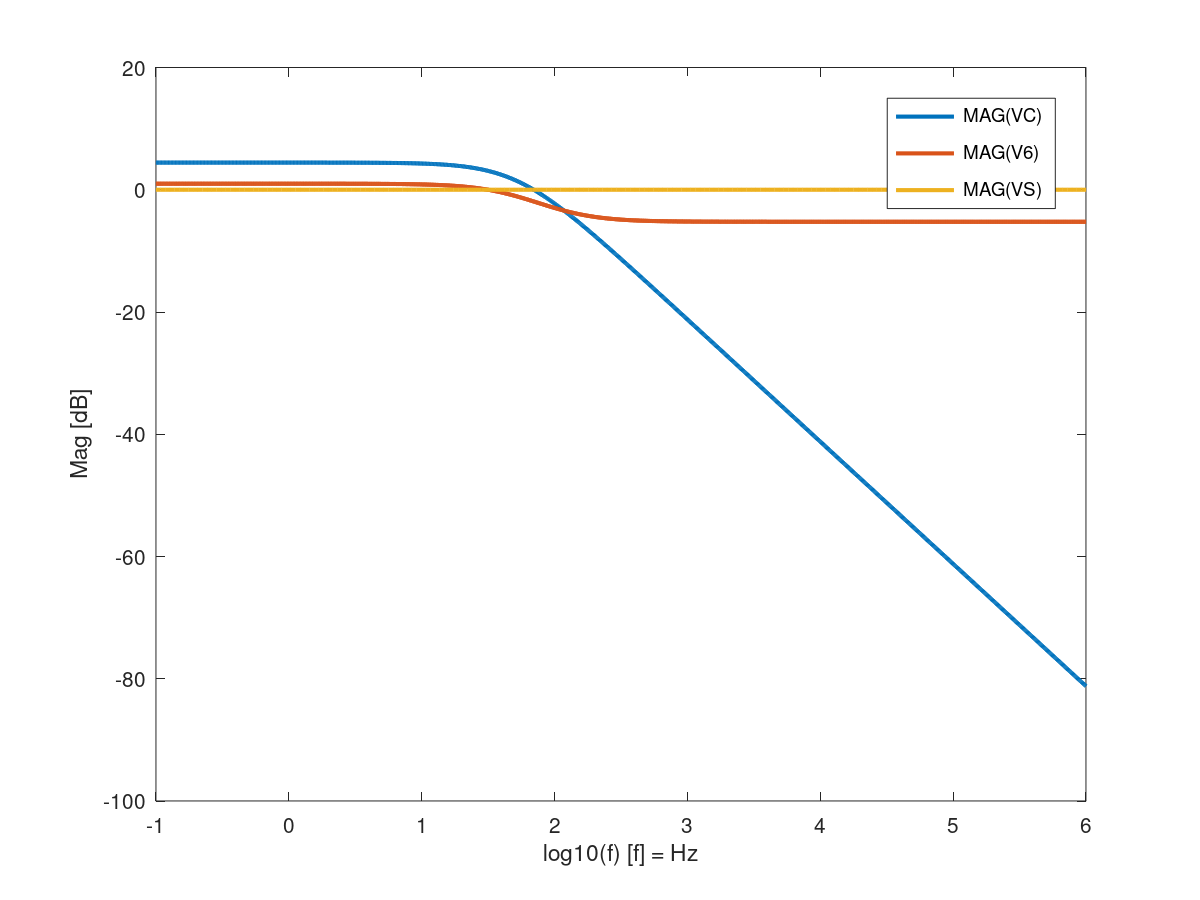
\includegraphics[width=.6\textwidth]{../mat/vcmag.png} \label{fig:teo_mag} 
  } 
  \subfigure[Simulation analysis]{% 
    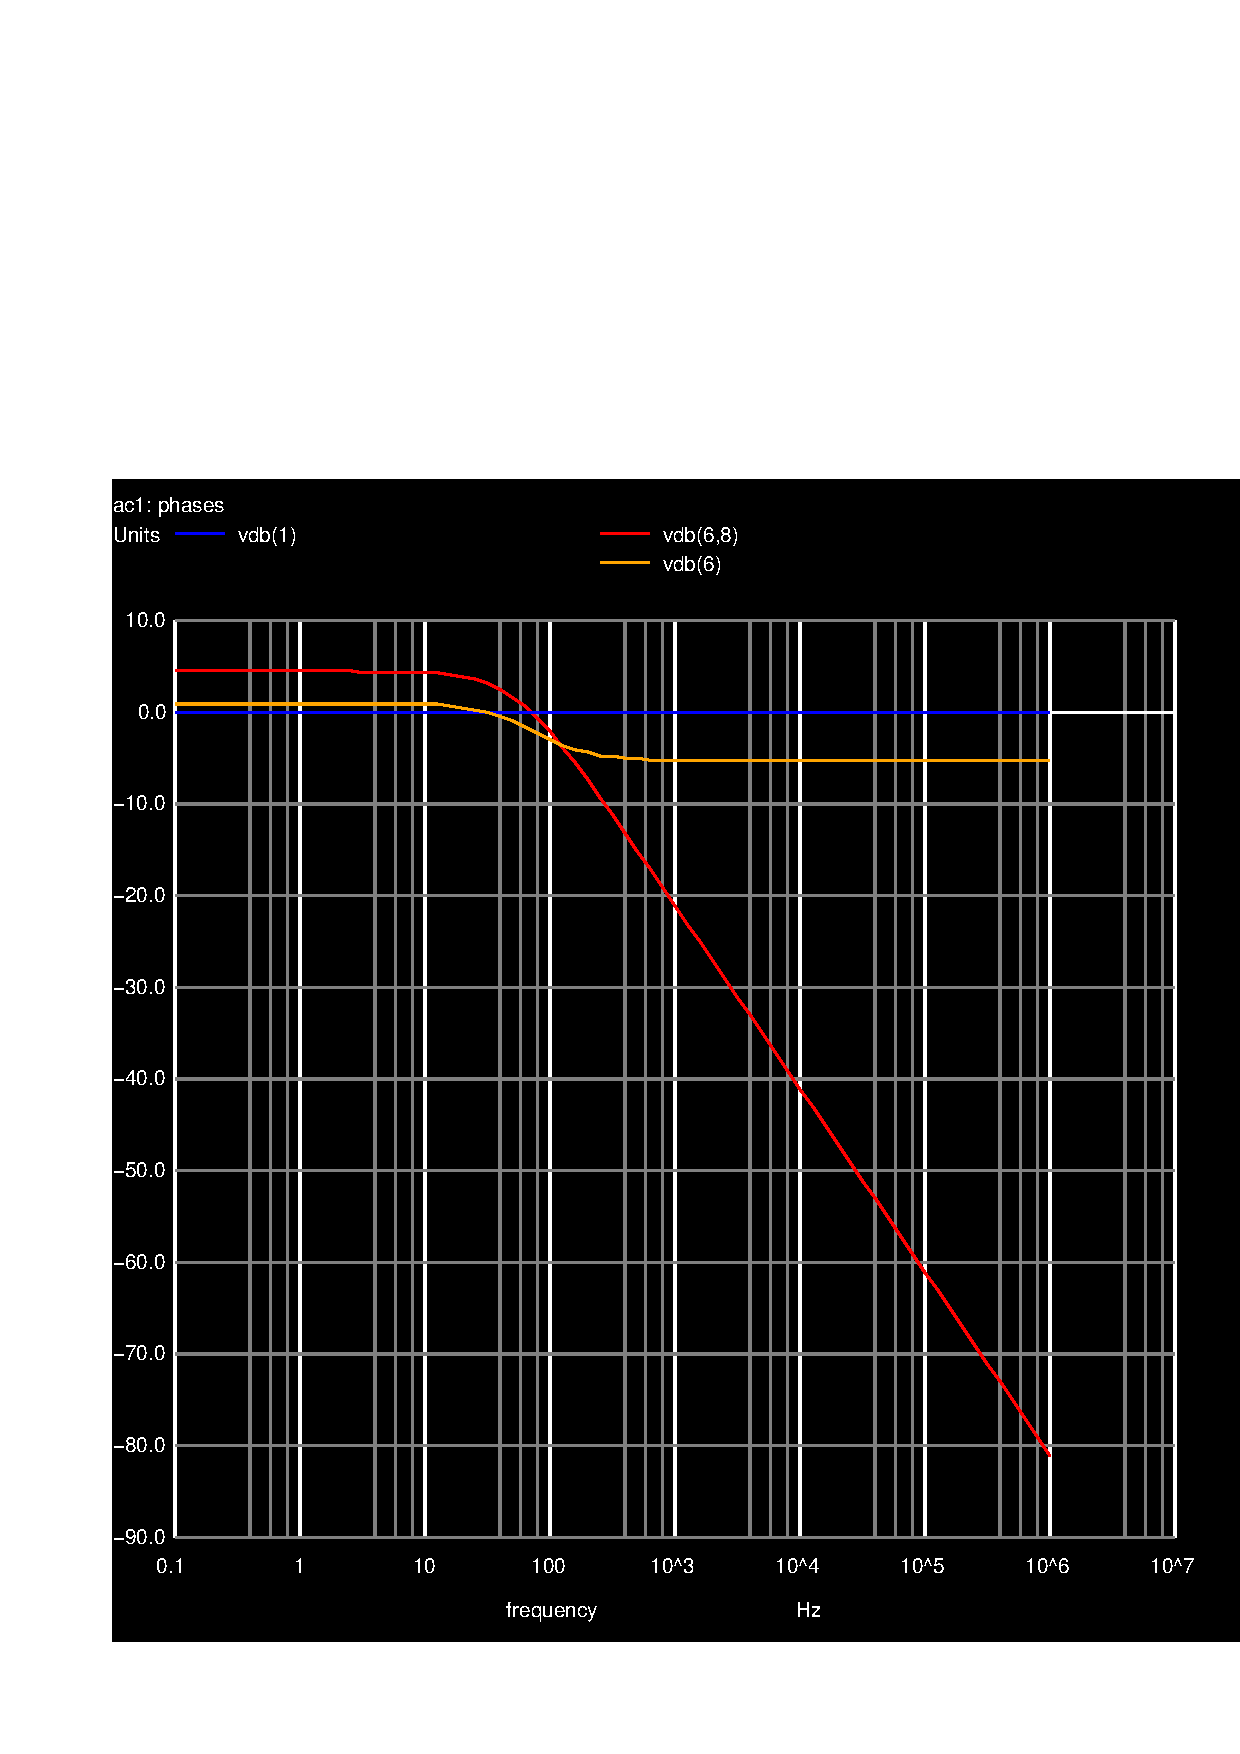
\includegraphics[width=.45\textwidth]{../sim/voltage_mag.pdf} \label{fig:sim_mag} 
  } 
  \caption{Magnitude as a function of the frequency of the voltage source.} 
  Once again no differences can be found between the 2 plots.
  
\end{figure}
\section{Conclusion}
In this laboratory assignment, as presented above, we were proposed to build and study the behaviour of an AC/DC converter. To build it, one used an envelope detector circuit (composed by a full-wave rectifier which turns the AC input into a DC output and a capacitor which smooths the oscillating current) and a voltage regulator circuit (that uses a resistor and multiple diodes which limit the output voltage to the desired value - 12V).\\

To evaluate how good the built converter was, we recurred the merit score presented in \eqref{score}. The results obtained in the simulation analysis (section 2) were very satisfactory except the stabilization time of the circuit, but that wasn't taken into account in the score obtained for the circuit although we had in mind that the circuit shouldn't have a very long stabilization time. The results given by the simulation analysis show an output signal with an average value displaced $\sim 10^{-7}$V from the desired value of 12V and with ripples $\sim 10^{-4}$V. The output voltage obtained is thus almost perfectly equal to the desired output voltage for this converter, which shows that the goal of this simulation was successfully achieved.\\

Comparing the simulation and the theoretical results one can notice a significant difference between the plots and the results obtained with both as anticipated on section 2. In fact, this phenomenon can be justified by the multiple approximations made in the theoretical analysis, namely on the diode model used. In the analysis made using \textit{Octave}, one used the diode models presented in class which neglect the non-linear behaviour of these components which ends up introducing discrepancies between the analysis methods used.\\

However, it is also important to notice that the results obtained on the theoretical analysis were affected of very small ripples, not however as small as in the simulation. To get a better approximation of the merit obtained in the simulation part, we proposed a corrected merit as well, which assumes that the average of the output voltage is exactly $12V$.\\

Therefore, and having explained the differences registered between the theoretical and the simulation analysis, it can be stated that the goals for this laboratory assignment were successfully achieved.
\begin{thebibliography}{9}
\bibitem{ngsite} 
Ngspice official website, \textit{http://ngspice.sourceforge.net/}
\end{thebibliography}


\end{document}
